\documentclass[twoside]{book}

% Packages required by doxygen
\usepackage{fixltx2e}
\usepackage{calc}
\usepackage{doxygen}
\usepackage[export]{adjustbox} % also loads graphicx
\usepackage{graphicx}
\usepackage[utf8]{inputenc}
\usepackage{makeidx}
\usepackage{multicol}
\usepackage{multirow}
\PassOptionsToPackage{warn}{textcomp}
\usepackage{textcomp}
\usepackage[nointegrals]{wasysym}
\usepackage[table]{xcolor}

% Font selection
\usepackage[T1]{fontenc}
\usepackage[scaled=.90]{helvet}
\usepackage{courier}
\usepackage{amssymb}
\usepackage{sectsty}
\renewcommand{\familydefault}{\sfdefault}
\allsectionsfont{%
  \fontseries{bc}\selectfont%
  \color{darkgray}%
}
\renewcommand{\DoxyLabelFont}{%
  \fontseries{bc}\selectfont%
  \color{darkgray}%
}
\newcommand{\+}{\discretionary{\mbox{\scriptsize$\hookleftarrow$}}{}{}}

% Page & text layout
\usepackage{geometry}
\geometry{%
  a4paper,%
  top=2.5cm,%
  bottom=2.5cm,%
  left=2.5cm,%
  right=2.5cm%
}
\tolerance=750
\hfuzz=15pt
\hbadness=750
\setlength{\emergencystretch}{15pt}
\setlength{\parindent}{0cm}
\setlength{\parskip}{3ex plus 2ex minus 2ex}
\makeatletter
\renewcommand{\paragraph}{%
  \@startsection{paragraph}{4}{0ex}{-1.0ex}{1.0ex}{%
    \normalfont\normalsize\bfseries\SS@parafont%
  }%
}
\renewcommand{\subparagraph}{%
  \@startsection{subparagraph}{5}{0ex}{-1.0ex}{1.0ex}{%
    \normalfont\normalsize\bfseries\SS@subparafont%
  }%
}
\makeatother

% Headers & footers
\usepackage{fancyhdr}
\pagestyle{fancyplain}
\fancyhead[LE]{\fancyplain{}{\bfseries\thepage}}
\fancyhead[CE]{\fancyplain{}{}}
\fancyhead[RE]{\fancyplain{}{\bfseries\leftmark}}
\fancyhead[LO]{\fancyplain{}{\bfseries\rightmark}}
\fancyhead[CO]{\fancyplain{}{}}
\fancyhead[RO]{\fancyplain{}{\bfseries\thepage}}
\fancyfoot[LE]{\fancyplain{}{}}
\fancyfoot[CE]{\fancyplain{}{}}
\fancyfoot[RE]{\fancyplain{}{\bfseries\scriptsize Generated by Doxygen }}
\fancyfoot[LO]{\fancyplain{}{\bfseries\scriptsize Generated by Doxygen }}
\fancyfoot[CO]{\fancyplain{}{}}
\fancyfoot[RO]{\fancyplain{}{}}
\renewcommand{\footrulewidth}{0.4pt}
\renewcommand{\chaptermark}[1]{%
  \markboth{#1}{}%
}
\renewcommand{\sectionmark}[1]{%
  \markright{\thesection\ #1}%
}

% Indices & bibliography
\usepackage{natbib}
\usepackage[titles]{tocloft}
\setcounter{tocdepth}{3}
\setcounter{secnumdepth}{5}
\makeindex

% Hyperlinks (required, but should be loaded last)
\usepackage{ifpdf}
\ifpdf
  \usepackage[pdftex,pagebackref=true]{hyperref}
\else
  \usepackage[ps2pdf,pagebackref=true]{hyperref}
\fi
\hypersetup{%
  colorlinks=true,%
  linkcolor=blue,%
  citecolor=blue,%
  unicode%
}

% Custom commands
\newcommand{\clearemptydoublepage}{%
  \newpage{\pagestyle{empty}\cleardoublepage}%
}

\usepackage{caption}
\captionsetup{labelsep=space,justification=centering,font={bf},singlelinecheck=off,skip=4pt,position=top}

%===== C O N T E N T S =====

\begin{document}

% Titlepage & ToC
\hypersetup{pageanchor=false,
             bookmarksnumbered=true,
             pdfencoding=unicode
            }
\pagenumbering{alph}
\begin{titlepage}
\vspace*{7cm}
\begin{center}%
{\Large Theoria }\\
\vspace*{1cm}
{\large Generated by Doxygen 1.8.13}\\
\end{center}
\end{titlepage}
\clearemptydoublepage
\pagenumbering{roman}
\tableofcontents
\clearemptydoublepage
\pagenumbering{arabic}
\hypersetup{pageanchor=true}

%--- Begin generated contents ---
\chapter{Hierarchical Index}
\section{Class Hierarchy}
This inheritance list is sorted roughly, but not completely, alphabetically\+:\begin{DoxyCompactList}
\item \contentsline{section}{theoria\+:\+:config\+:\+:Config\+:\+:Attr}{\pageref{structtheoria_1_1config_1_1Config_1_1Attr}}{}
\item \contentsline{section}{theoria\+:\+:core\+:\+:Bootstrap}{\pageref{classtheoria_1_1core_1_1Bootstrap}}{}
\item \contentsline{section}{theoria\+:\+:util\+:\+:Command\+Line}{\pageref{classtheoria_1_1util_1_1CommandLine}}{}
\item \contentsline{section}{theoria\+:\+:core\+:\+:Component}{\pageref{classtheoria_1_1core_1_1Component}}{}
\begin{DoxyCompactList}
\item \contentsline{section}{theoria\+:\+:core\+:\+:App\+Config\+Resolver\+Comp}{\pageref{classtheoria_1_1core_1_1AppConfigResolverComp}}{}
\item \contentsline{section}{theoria\+:\+:core\+:\+:Cmd\+Line\+Resolver\+Comp}{\pageref{classtheoria_1_1core_1_1CmdLineResolverComp}}{}
\item \contentsline{section}{theoria\+:\+:core\+:\+:Config\+Var\+Resolver\+Builder\+Comp}{\pageref{classtheoria_1_1core_1_1ConfigVarResolverBuilderComp}}{}
\item \contentsline{section}{theoria\+:\+:core\+:\+:Env\+Var\+Resolver\+Comp}{\pageref{classtheoria_1_1core_1_1EnvVarResolverComp}}{}
\item \contentsline{section}{theoria\+:\+:core\+:\+:T\+O\+M\+L\+Config\+Builder\+Comp}{\pageref{classtheoria_1_1core_1_1TOMLConfigBuilderComp}}{}
\end{DoxyCompactList}
\item Component\begin{DoxyCompactList}
\item \contentsline{section}{Config\+Resolver\+Builder}{\pageref{classConfigResolverBuilder}}{}
\end{DoxyCompactList}
\item \contentsline{section}{theoria\+:\+:core\+:\+:Component\+Data}{\pageref{classtheoria_1_1core_1_1ComponentData}}{}
\item \contentsline{section}{theoria\+:\+:core\+:\+:Comp\+State}{\pageref{classtheoria_1_1core_1_1CompState}}{}
\item \contentsline{section}{theoria\+:\+:config\+:\+:Config}{\pageref{classtheoria_1_1config_1_1Config}}{}
\begin{DoxyCompactList}
\item \contentsline{section}{theoria\+:\+:config\+:\+:Config\+Array}{\pageref{classtheoria_1_1config_1_1ConfigArray}}{}
\end{DoxyCompactList}
\item \contentsline{section}{theoria\+:\+:config\+:\+:Config\+Builder}{\pageref{classtheoria_1_1config_1_1ConfigBuilder}}{}
\begin{DoxyCompactList}
\item \contentsline{section}{theoria\+:\+:config\+:\+:T\+O\+M\+L\+Config\+Builder}{\pageref{classtheoria_1_1config_1_1TOMLConfigBuilder}}{}
\end{DoxyCompactList}
\item \contentsline{section}{theoria\+:\+:config\+:\+:Config\+Parser}{\pageref{classtheoria_1_1config_1_1ConfigParser}}{}
\begin{DoxyCompactList}
\item \contentsline{section}{theoria\+:\+:config\+:\+:T\+O\+M\+L\+Config\+Builder}{\pageref{classtheoria_1_1config_1_1TOMLConfigBuilder}}{}
\end{DoxyCompactList}
\item \contentsline{section}{theoria\+:\+:config\+:\+:Config\+Variable\+Resolver}{\pageref{classtheoria_1_1config_1_1ConfigVariableResolver}}{}
\begin{DoxyCompactList}
\item \contentsline{section}{theoria\+:\+:config\+:\+:Cmd\+Line\+Resolver}{\pageref{classtheoria_1_1config_1_1CmdLineResolver}}{}
\item \contentsline{section}{theoria\+:\+:config\+:\+:Disable\+Resolver}{\pageref{classtheoria_1_1config_1_1DisableResolver}}{}
\item \contentsline{section}{theoria\+:\+:config\+:\+:Disallow\+Resolver}{\pageref{classtheoria_1_1config_1_1DisallowResolver}}{}
\item \contentsline{section}{theoria\+:\+:config\+:\+:Env\+Var\+Resolver}{\pageref{classtheoria_1_1config_1_1EnvVarResolver}}{}
\item \contentsline{section}{theoria\+:\+:config\+:\+:T\+O\+M\+L\+Resolver}{\pageref{classtheoria_1_1config_1_1TOMLResolver}}{}
\item \contentsline{section}{theoria\+:\+:core\+:\+:App\+Config\+Resolver}{\pageref{classtheoria_1_1core_1_1AppConfigResolver}}{}
\item \contentsline{section}{theoria\+:\+:config\+:\+:T\+O\+M\+L\+Resolver\+:\+:T\+O\+M\+L\+Resolver\+Impl}{\pageref{classTOMLResolver_1_1TOMLResolverImpl}}{}
\end{DoxyCompactList}
\item \contentsline{section}{theoria\+:\+:util\+:\+:densemap$<$ K\+EY, T, Alloc $>$\+:\+:Const\+Iter}{\pageref{classtheoria_1_1util_1_1densemap_1_1ConstIter}}{}
\item \contentsline{section}{theoria\+:\+:util\+:\+:densemap$<$ K\+EY, T, Alloc $>$}{\pageref{classtheoria_1_1util_1_1densemap}}{}
\item \contentsline{section}{theoria\+:\+:util\+:\+:densemap$<$ Comp\+Id, Component $\ast$ $>$}{\pageref{classtheoria_1_1util_1_1densemap}}{}
\item \contentsline{section}{theoria\+:\+:core\+:\+:Dependencies}{\pageref{classtheoria_1_1core_1_1Dependencies}}{}
\item \contentsline{section}{theoria\+:\+:core\+:\+:Dependencies\+:\+:Dependent}{\pageref{structtheoria_1_1core_1_1Dependencies_1_1Dependent}}{}
\item std\+:\+:exception\begin{DoxyCompactList}
\item \contentsline{section}{theoria\+:\+:core\+:\+:Registry\+Locked}{\pageref{classtheoria_1_1core_1_1RegistryLocked}}{}
\end{DoxyCompactList}
\item \contentsline{section}{theoria\+:\+:util\+:\+:densemap$<$ K\+EY, T, Alloc $>$\+:\+:Iter}{\pageref{classtheoria_1_1util_1_1densemap_1_1Iter}}{}
\item \contentsline{section}{theoria\+:\+:util\+:\+:Maybe$<$ T $>$}{\pageref{classtheoria_1_1util_1_1Maybe}}{}
\item \contentsline{section}{theoria\+:\+:core\+:\+:Message}{\pageref{classtheoria_1_1core_1_1Message}}{}
\item \contentsline{section}{theoria\+:\+:core\+:\+:Msg\+Data}{\pageref{uniontheoria_1_1core_1_1MsgData}}{}
\item \contentsline{section}{theoria\+:\+:core\+:\+:Register\+This$<$ T\+Comp $>$}{\pageref{classtheoria_1_1core_1_1RegisterThis}}{}
\item \contentsline{section}{theoria\+:\+:core\+:\+:Register\+This$<$ theoria\+:\+:core\+:\+:App\+Config\+Resolver\+Comp $>$}{\pageref{classtheoria_1_1core_1_1RegisterThis}}{}
\item \contentsline{section}{theoria\+:\+:core\+:\+:Register\+This$<$ theoria\+:\+:core\+:\+:Cmd\+Line\+Resolver\+Comp $>$}{\pageref{classtheoria_1_1core_1_1RegisterThis}}{}
\item \contentsline{section}{theoria\+:\+:core\+:\+:Register\+This$<$ theoria\+:\+:core\+:\+:Config\+Var\+Resolver\+Builder\+Comp $>$}{\pageref{classtheoria_1_1core_1_1RegisterThis}}{}
\item \contentsline{section}{theoria\+:\+:core\+:\+:Register\+This$<$ theoria\+:\+:core\+:\+:Env\+Var\+Resolver\+Comp $>$}{\pageref{classtheoria_1_1core_1_1RegisterThis}}{}
\item \contentsline{section}{theoria\+:\+:core\+:\+:Register\+This$<$ theoria\+:\+:core\+:\+:T\+O\+M\+L\+Config\+Builder\+Comp $>$}{\pageref{classtheoria_1_1core_1_1RegisterThis}}{}
\item \contentsline{section}{theoria\+:\+:core\+:\+:Registry}{\pageref{classtheoria_1_1core_1_1Registry}}{}
\item \contentsline{section}{theoria\+:\+:core\+:\+:Registry\+Lock}{\pageref{structtheoria_1_1core_1_1RegistryLock}}{}
\item \contentsline{section}{theoria\+:\+:core\+:\+:Theoria}{\pageref{classtheoria_1_1core_1_1Theoria}}{}
\item \contentsline{section}{to\+Toml\+Name}{\pageref{structtoTomlName}}{}
\end{DoxyCompactList}

\chapter{Class Index}
\section{Class List}
Here are the classes, structs, unions and interfaces with brief descriptions\+:\begin{DoxyCompactList}
\item\contentsline{section}{\hyperlink{classtheoria_1_1core_1_1AppConfigResolver}{theoria\+::core\+::\+App\+Config\+Resolver} }{\pageref{classtheoria_1_1core_1_1AppConfigResolver}}{}
\item\contentsline{section}{\hyperlink{structtheoria_1_1config_1_1Config_1_1Attr}{theoria\+::config\+::\+Config\+::\+Attr} }{\pageref{structtheoria_1_1config_1_1Config_1_1Attr}}{}
\item\contentsline{section}{\hyperlink{classtheoria_1_1core_1_1Bootstrap}{theoria\+::core\+::\+Bootstrap} }{\pageref{classtheoria_1_1core_1_1Bootstrap}}{}
\item\contentsline{section}{\hyperlink{classtheoria_1_1config_1_1CmdLineResolver}{theoria\+::config\+::\+Cmd\+Line\+Resolver} }{\pageref{classtheoria_1_1config_1_1CmdLineResolver}}{}
\item\contentsline{section}{\hyperlink{classtheoria_1_1util_1_1CommandLine}{theoria\+::util\+::\+Command\+Line} }{\pageref{classtheoria_1_1util_1_1CommandLine}}{}
\item\contentsline{section}{\hyperlink{classtheoria_1_1core_1_1Component}{theoria\+::core\+::\+Component} }{\pageref{classtheoria_1_1core_1_1Component}}{}
\item\contentsline{section}{\hyperlink{classtheoria_1_1core_1_1ComponentData}{theoria\+::core\+::\+Component\+Data} }{\pageref{classtheoria_1_1core_1_1ComponentData}}{}
\item\contentsline{section}{\hyperlink{classtheoria_1_1core_1_1CompState}{theoria\+::core\+::\+Comp\+State} }{\pageref{classtheoria_1_1core_1_1CompState}}{}
\item\contentsline{section}{\hyperlink{classtheoria_1_1config_1_1Config}{theoria\+::config\+::\+Config} }{\pageref{classtheoria_1_1config_1_1Config}}{}
\item\contentsline{section}{\hyperlink{classtheoria_1_1config_1_1ConfigArray}{theoria\+::config\+::\+Config\+Array} }{\pageref{classtheoria_1_1config_1_1ConfigArray}}{}
\item\contentsline{section}{\hyperlink{classtheoria_1_1config_1_1ConfigBuilder}{theoria\+::config\+::\+Config\+Builder} }{\pageref{classtheoria_1_1config_1_1ConfigBuilder}}{}
\item\contentsline{section}{\hyperlink{classtheoria_1_1config_1_1ConfigParser}{theoria\+::config\+::\+Config\+Parser} }{\pageref{classtheoria_1_1config_1_1ConfigParser}}{}
\item\contentsline{section}{\hyperlink{classConfigResolverBuilder}{Config\+Resolver\+Builder} }{\pageref{classConfigResolverBuilder}}{}
\item\contentsline{section}{\hyperlink{classtheoria_1_1config_1_1ConfigVariableResolver}{theoria\+::config\+::\+Config\+Variable\+Resolver} }{\pageref{classtheoria_1_1config_1_1ConfigVariableResolver}}{}
\item\contentsline{section}{\hyperlink{classtheoria_1_1core_1_1ConfigVarResolverBuilderComp}{theoria\+::core\+::\+Config\+Var\+Resolver\+Builder\+Comp} }{\pageref{classtheoria_1_1core_1_1ConfigVarResolverBuilderComp}}{}
\item\contentsline{section}{\hyperlink{classtheoria_1_1util_1_1densemap_1_1ConstIter}{theoria\+::util\+::densemap$<$ K\+E\+Y, T, Alloc $>$\+::\+Const\+Iter} }{\pageref{classtheoria_1_1util_1_1densemap_1_1ConstIter}}{}
\item\contentsline{section}{\hyperlink{classtheoria_1_1util_1_1densemap}{theoria\+::util\+::densemap$<$ K\+E\+Y, T, Alloc $>$} }{\pageref{classtheoria_1_1util_1_1densemap}}{}
\item\contentsline{section}{\hyperlink{classtheoria_1_1core_1_1Dependencies}{theoria\+::core\+::\+Dependencies} }{\pageref{classtheoria_1_1core_1_1Dependencies}}{}
\item\contentsline{section}{\hyperlink{structtheoria_1_1core_1_1Dependencies_1_1Dependent}{theoria\+::core\+::\+Dependencies\+::\+Dependent} }{\pageref{structtheoria_1_1core_1_1Dependencies_1_1Dependent}}{}
\item\contentsline{section}{\hyperlink{classtheoria_1_1config_1_1DisableResolver}{theoria\+::config\+::\+Disable\+Resolver} }{\pageref{classtheoria_1_1config_1_1DisableResolver}}{}
\item\contentsline{section}{\hyperlink{classtheoria_1_1config_1_1DisallowResolver}{theoria\+::config\+::\+Disallow\+Resolver} }{\pageref{classtheoria_1_1config_1_1DisallowResolver}}{}
\item\contentsline{section}{\hyperlink{classtheoria_1_1config_1_1EnvVarResolver}{theoria\+::config\+::\+Env\+Var\+Resolver} }{\pageref{classtheoria_1_1config_1_1EnvVarResolver}}{}
\item\contentsline{section}{\hyperlink{classtheoria_1_1util_1_1densemap_1_1Iter}{theoria\+::util\+::densemap$<$ K\+E\+Y, T, Alloc $>$\+::\+Iter} }{\pageref{classtheoria_1_1util_1_1densemap_1_1Iter}}{}
\item\contentsline{section}{\hyperlink{classtheoria_1_1util_1_1Maybe}{theoria\+::util\+::\+Maybe$<$ T $>$} }{\pageref{classtheoria_1_1util_1_1Maybe}}{}
\item\contentsline{section}{\hyperlink{classtheoria_1_1core_1_1Message}{theoria\+::core\+::\+Message} }{\pageref{classtheoria_1_1core_1_1Message}}{}
\item\contentsline{section}{\hyperlink{uniontheoria_1_1core_1_1MsgData}{theoria\+::core\+::\+Msg\+Data} }{\pageref{uniontheoria_1_1core_1_1MsgData}}{}
\item\contentsline{section}{\hyperlink{classtheoria_1_1core_1_1RegisterThis}{theoria\+::core\+::\+Register\+This$<$ T\+Comp $>$} }{\pageref{classtheoria_1_1core_1_1RegisterThis}}{}
\item\contentsline{section}{\hyperlink{classtheoria_1_1core_1_1Registry}{theoria\+::core\+::\+Registry} }{\pageref{classtheoria_1_1core_1_1Registry}}{}
\item\contentsline{section}{\hyperlink{structtheoria_1_1core_1_1RegistryLock}{theoria\+::core\+::\+Registry\+Lock} }{\pageref{structtheoria_1_1core_1_1RegistryLock}}{}
\item\contentsline{section}{\hyperlink{classtheoria_1_1core_1_1Theoria}{theoria\+::core\+::\+Theoria} }{\pageref{classtheoria_1_1core_1_1Theoria}}{}
\item\contentsline{section}{\hyperlink{classtheoria_1_1config_1_1TOMLConfigBuilder}{theoria\+::config\+::\+T\+O\+M\+L\+Config\+Builder} }{\pageref{classtheoria_1_1config_1_1TOMLConfigBuilder}}{}
\item\contentsline{section}{\hyperlink{classtheoria_1_1config_1_1TOMLResolver}{theoria\+::config\+::\+T\+O\+M\+L\+Resolver} }{\pageref{classtheoria_1_1config_1_1TOMLResolver}}{}
\item\contentsline{section}{\hyperlink{classTOMLResolver_1_1TOMLResolverImpl}{theoria\+::config\+::\+T\+O\+M\+L\+Resolver\+::\+T\+O\+M\+L\+Resolver\+Impl} }{\pageref{classTOMLResolver_1_1TOMLResolverImpl}}{}
\item\contentsline{section}{\hyperlink{structtoTomlName}{to\+Toml\+Name} }{\pageref{structtoTomlName}}{}
\end{DoxyCompactList}

\chapter{Class Documentation}
\hypertarget{classtheoria_1_1core_1_1AppConfigResolver}{}\section{theoria\+:\+:core\+:\+:App\+Config\+Resolver Class Reference}
\label{classtheoria_1_1core_1_1AppConfigResolver}\index{theoria\+::core\+::\+App\+Config\+Resolver@{theoria\+::core\+::\+App\+Config\+Resolver}}


Inheritance diagram for theoria\+:\+:core\+:\+:App\+Config\+Resolver\+:
\nopagebreak
\begin{figure}[H]
\begin{center}
\leavevmode
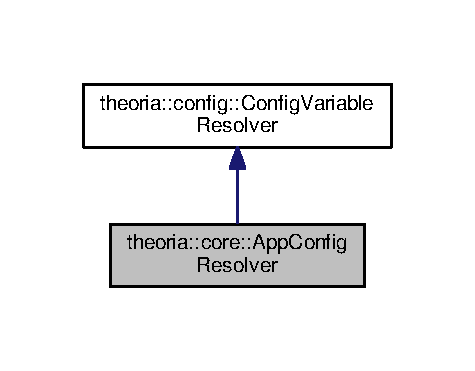
\includegraphics[width=228pt]{classtheoria_1_1core_1_1AppConfigResolver__inherit__graph}
\end{center}
\end{figure}


Collaboration diagram for theoria\+:\+:core\+:\+:App\+Config\+Resolver\+:
\nopagebreak
\begin{figure}[H]
\begin{center}
\leavevmode
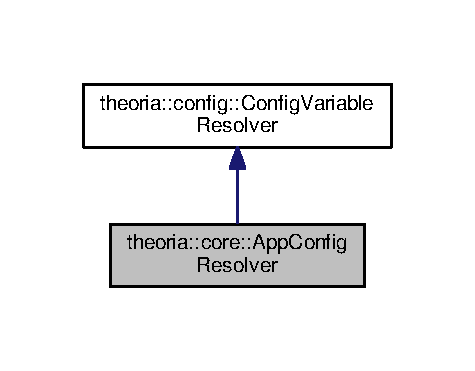
\includegraphics[width=228pt]{classtheoria_1_1core_1_1AppConfigResolver__coll__graph}
\end{center}
\end{figure}
\subsection*{Public Member Functions}
\begin{DoxyCompactItemize}
\item 
\mbox{\Hypertarget{classtheoria_1_1core_1_1AppConfigResolver_a7922df9559e63ccd91db5177224823fc}\label{classtheoria_1_1core_1_1AppConfigResolver_a7922df9559e63ccd91db5177224823fc}} 
Result {\bfseries lookup} (const std\+::string \&\hyperlink{classtheoria_1_1core_1_1AppConfigResolver_ad7c8c08e622613c6505418774a71abda}{name}) const override
\item 
virtual std\+::string \hyperlink{classtheoria_1_1core_1_1AppConfigResolver_ad7c8c08e622613c6505418774a71abda}{name} () const override
\end{DoxyCompactItemize}
\subsection*{Additional Inherited Members}


\subsection{Member Function Documentation}
\mbox{\Hypertarget{classtheoria_1_1core_1_1AppConfigResolver_ad7c8c08e622613c6505418774a71abda}\label{classtheoria_1_1core_1_1AppConfigResolver_ad7c8c08e622613c6505418774a71abda}} 
\index{theoria\+::core\+::\+App\+Config\+Resolver@{theoria\+::core\+::\+App\+Config\+Resolver}!name@{name}}
\index{name@{name}!theoria\+::core\+::\+App\+Config\+Resolver@{theoria\+::core\+::\+App\+Config\+Resolver}}
\subsubsection{\texorpdfstring{name()}{name()}}
{\footnotesize\ttfamily std\+::string App\+Config\+Resolver\+::name (\begin{DoxyParamCaption}{ }\end{DoxyParamCaption}) const\hspace{0.3cm}{\ttfamily [override]}, {\ttfamily [virtual]}}

Return name of the resolver 

Implements \hyperlink{classtheoria_1_1config_1_1ConfigVariableResolver_a026bda729faf988eaef334a45ec92303}{theoria\+::config\+::\+Config\+Variable\+Resolver}.



The documentation for this class was generated from the following files\+:\begin{DoxyCompactItemize}
\item 
include/theoria/core/App\+Config\+Resolver.\+h\item 
src/core/App\+Config\+Resolver.\+cpp\end{DoxyCompactItemize}

\hypertarget{classtheoria_1_1core_1_1AppConfigResolverComp}{}\section{theoria\+:\+:core\+:\+:App\+Config\+Resolver\+Comp Class Reference}
\label{classtheoria_1_1core_1_1AppConfigResolverComp}\index{theoria\+::core\+::\+App\+Config\+Resolver\+Comp@{theoria\+::core\+::\+App\+Config\+Resolver\+Comp}}


{\ttfamily \#include $<$Core\+Components.\+h$>$}



Inheritance diagram for theoria\+:\+:core\+:\+:App\+Config\+Resolver\+Comp\+:\nopagebreak
\begin{figure}[H]
\begin{center}
\leavevmode
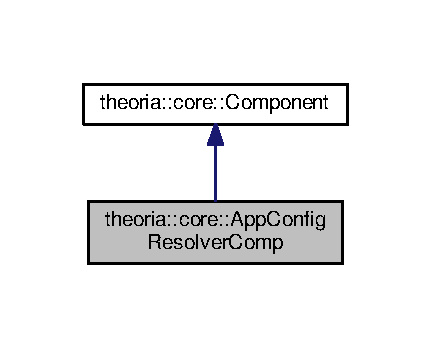
\includegraphics[width=207pt]{classtheoria_1_1core_1_1AppConfigResolverComp__inherit__graph}
\end{center}
\end{figure}


Collaboration diagram for theoria\+:\+:core\+:\+:App\+Config\+Resolver\+Comp\+:\nopagebreak
\begin{figure}[H]
\begin{center}
\leavevmode
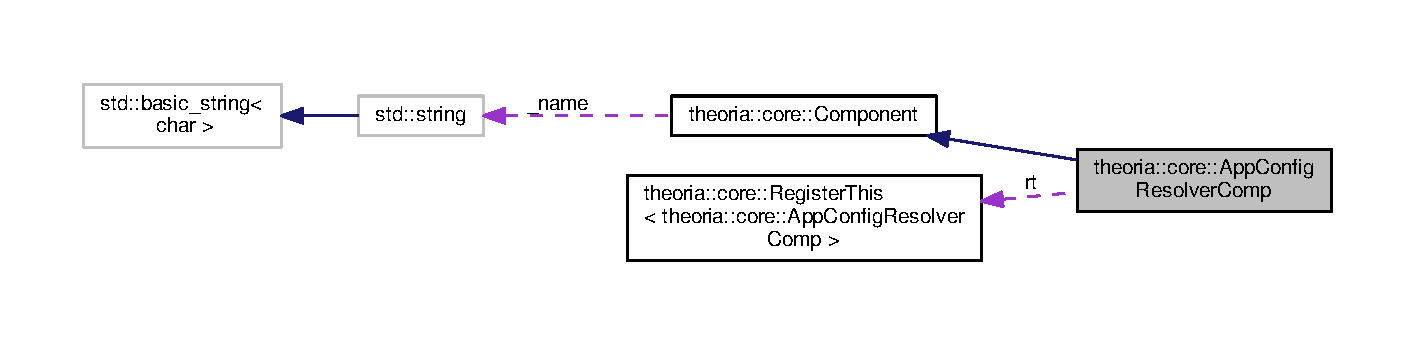
\includegraphics[width=350pt]{classtheoria_1_1core_1_1AppConfigResolverComp__coll__graph}
\end{center}
\end{figure}
\subsection*{Public Member Functions}
\begin{DoxyCompactItemize}
\item 
\hyperlink{classtheoria_1_1core_1_1AppConfigResolverComp_a49f449b95efaa632d5398b161b28144e}{App\+Config\+Resolver\+Comp} (Comp\+Id \hyperlink{classtheoria_1_1core_1_1Component_ab539df9f996efceda7743fa1b69cd25d}{id})
\item 
\hyperlink{classtheoria_1_1core_1_1Component}{Component} $\ast$ \hyperlink{classtheoria_1_1core_1_1AppConfigResolverComp_af04af67f66e3bfea44ab76c33d64a51e}{acquire} (const std\+::type\+\_\+info \&type\+Info, void $\ast$$\ast$dest) override
\end{DoxyCompactItemize}
\subsection*{Static Public Member Functions}
\begin{DoxyCompactItemize}
\item 
static \hyperlink{classtheoria_1_1core_1_1Component}{Component} $\ast$ \hyperlink{classtheoria_1_1core_1_1AppConfigResolverComp_aa439f83c466b28a3d1df82cc106f87b4}{factory} (Comp\+Id \hyperlink{classtheoria_1_1core_1_1Component_ab539df9f996efceda7743fa1b69cd25d}{id})
\end{DoxyCompactItemize}
\subsection*{Static Public Attributes}
\begin{DoxyCompactItemize}
\item 
static D\+L\+L\+\_\+\+P\+U\+B\+L\+IC \hyperlink{classtheoria_1_1core_1_1RegisterThis}{Register\+This}$<$ \hyperlink{classtheoria_1_1core_1_1AppConfigResolverComp}{App\+Config\+Resolver\+Comp} $>$ \hyperlink{classtheoria_1_1core_1_1AppConfigResolverComp_a25d3ff11e2e50221cd2755fbc8feb313}{rt}
\end{DoxyCompactItemize}
\subsection*{Additional Inherited Members}


\subsection{Detailed Description}
\hyperlink{classtheoria_1_1core_1_1Component}{Component} wrapper to a \hyperlink{classtheoria_1_1core_1_1AppConfigResolver}{App\+Config\+Resolver} 

\subsection{Constructor \& Destructor Documentation}
\mbox{\Hypertarget{classtheoria_1_1core_1_1AppConfigResolverComp_a49f449b95efaa632d5398b161b28144e}\label{classtheoria_1_1core_1_1AppConfigResolverComp_a49f449b95efaa632d5398b161b28144e}} 
\index{theoria\+::core\+::\+App\+Config\+Resolver\+Comp@{theoria\+::core\+::\+App\+Config\+Resolver\+Comp}!App\+Config\+Resolver\+Comp@{App\+Config\+Resolver\+Comp}}
\index{App\+Config\+Resolver\+Comp@{App\+Config\+Resolver\+Comp}!theoria\+::core\+::\+App\+Config\+Resolver\+Comp@{theoria\+::core\+::\+App\+Config\+Resolver\+Comp}}
\subsubsection{\texorpdfstring{App\+Config\+Resolver\+Comp()}{AppConfigResolverComp()}}
{\footnotesize\ttfamily theoria\+::core\+::\+App\+Config\+Resolver\+Comp\+::\+App\+Config\+Resolver\+Comp (\begin{DoxyParamCaption}\item[{Comp\+Id}]{id }\end{DoxyParamCaption})\hspace{0.3cm}{\ttfamily [inline]}}

\hyperlink{classtheoria_1_1core_1_1Component}{Component} constructor 

\subsection{Member Function Documentation}
\mbox{\Hypertarget{classtheoria_1_1core_1_1AppConfigResolverComp_af04af67f66e3bfea44ab76c33d64a51e}\label{classtheoria_1_1core_1_1AppConfigResolverComp_af04af67f66e3bfea44ab76c33d64a51e}} 
\index{theoria\+::core\+::\+App\+Config\+Resolver\+Comp@{theoria\+::core\+::\+App\+Config\+Resolver\+Comp}!acquire@{acquire}}
\index{acquire@{acquire}!theoria\+::core\+::\+App\+Config\+Resolver\+Comp@{theoria\+::core\+::\+App\+Config\+Resolver\+Comp}}
\subsubsection{\texorpdfstring{acquire()}{acquire()}}
{\footnotesize\ttfamily \hyperlink{classtheoria_1_1core_1_1Component}{Component} $\ast$ App\+Config\+Resolver\+Comp\+::acquire (\begin{DoxyParamCaption}\item[{const std\+::type\+\_\+info \&}]{type\+Info,  }\item[{void $\ast$$\ast$}]{dest }\end{DoxyParamCaption})\hspace{0.3cm}{\ttfamily [override]}, {\ttfamily [virtual]}}

Used to acquire underlying resolver 

Reimplemented from \hyperlink{classtheoria_1_1core_1_1Component_a18744abc83e088af3c3d42e0a22c35e3}{theoria\+::core\+::\+Component}.

\mbox{\Hypertarget{classtheoria_1_1core_1_1AppConfigResolverComp_aa439f83c466b28a3d1df82cc106f87b4}\label{classtheoria_1_1core_1_1AppConfigResolverComp_aa439f83c466b28a3d1df82cc106f87b4}} 
\index{theoria\+::core\+::\+App\+Config\+Resolver\+Comp@{theoria\+::core\+::\+App\+Config\+Resolver\+Comp}!factory@{factory}}
\index{factory@{factory}!theoria\+::core\+::\+App\+Config\+Resolver\+Comp@{theoria\+::core\+::\+App\+Config\+Resolver\+Comp}}
\subsubsection{\texorpdfstring{factory()}{factory()}}
{\footnotesize\ttfamily \hyperlink{classtheoria_1_1core_1_1Component}{Component} $\ast$ App\+Config\+Resolver\+Comp\+::factory (\begin{DoxyParamCaption}\item[{Comp\+Id}]{id }\end{DoxyParamCaption})\hspace{0.3cm}{\ttfamily [static]}}

Factory for this component 

\subsection{Member Data Documentation}
\mbox{\Hypertarget{classtheoria_1_1core_1_1AppConfigResolverComp_a25d3ff11e2e50221cd2755fbc8feb313}\label{classtheoria_1_1core_1_1AppConfigResolverComp_a25d3ff11e2e50221cd2755fbc8feb313}} 
\index{theoria\+::core\+::\+App\+Config\+Resolver\+Comp@{theoria\+::core\+::\+App\+Config\+Resolver\+Comp}!rt@{rt}}
\index{rt@{rt}!theoria\+::core\+::\+App\+Config\+Resolver\+Comp@{theoria\+::core\+::\+App\+Config\+Resolver\+Comp}}
\subsubsection{\texorpdfstring{rt}{rt}}
{\footnotesize\ttfamily \hyperlink{classtheoria_1_1core_1_1RegisterThis}{Register\+This}$<$ \hyperlink{classtheoria_1_1core_1_1AppConfigResolverComp}{App\+Config\+Resolver\+Comp} $>$ App\+Config\+Resolver\+Comp\+::rt\hspace{0.3cm}{\ttfamily [static]}}

Register factory 

The documentation for this class was generated from the following files\+:\begin{DoxyCompactItemize}
\item 
include/theoria/core/Core\+Components.\+h\item 
src/core/Core\+Components.\+cpp\end{DoxyCompactItemize}

\hypertarget{structtheoria_1_1config_1_1Config_1_1Attr}{\section{theoria\+:\+:config\+:\+:Config\+:\+:Attr Struct Reference}
\label{structtheoria_1_1config_1_1Config_1_1Attr}\index{theoria\+::config\+::\+Config\+::\+Attr@{theoria\+::config\+::\+Config\+::\+Attr}}
}


Collaboration diagram for theoria\+:\+:config\+:\+:Config\+:\+:Attr\+:
\nopagebreak
\begin{figure}[H]
\begin{center}
\leavevmode
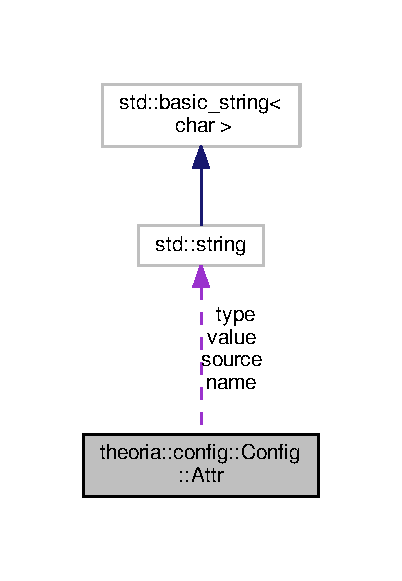
\includegraphics[width=193pt]{structtheoria_1_1config_1_1Config_1_1Attr__coll__graph}
\end{center}
\end{figure}
\subsection*{Public Member Functions}
\begin{DoxyCompactItemize}
\item 
\hypertarget{structtheoria_1_1config_1_1Config_1_1Attr_ab06451bb786404d66a1fce58229310f6}{{\bfseries Attr} (const std\+::string \&name\+\_\+, const std\+::string \&value\+\_\+, const std\+::string \&type\+\_\+=\char`\"{}\char`\"{}, const std\+::string \&src\+\_\+=\char`\"{}literal\char`\"{})}\label{structtheoria_1_1config_1_1Config_1_1Attr_ab06451bb786404d66a1fce58229310f6}

\item 
\hypertarget{structtheoria_1_1config_1_1Config_1_1Attr_a61bf523cf46cda0ba0d164527afd0d9a}{std\+::string {\bfseries decorated\+\_\+val} () const }\label{structtheoria_1_1config_1_1Config_1_1Attr_a61bf523cf46cda0ba0d164527afd0d9a}

\item 
\hypertarget{structtheoria_1_1config_1_1Config_1_1Attr_a833a679c41ba5783a1e1806054dadd68}{void {\bfseries to\+T\+O\+M\+L} (std\+::ostream \&os) const }\label{structtheoria_1_1config_1_1Config_1_1Attr_a833a679c41ba5783a1e1806054dadd68}

\end{DoxyCompactItemize}
\subsection*{Public Attributes}
\begin{DoxyCompactItemize}
\item 
\hypertarget{structtheoria_1_1config_1_1Config_1_1Attr_ad39ea60695427392538c9b70631e3893}{std\+::string {\bfseries name}}\label{structtheoria_1_1config_1_1Config_1_1Attr_ad39ea60695427392538c9b70631e3893}

\item 
\hypertarget{structtheoria_1_1config_1_1Config_1_1Attr_a089f492d8f4a5ca06879bef7dfc178f0}{std\+::string {\bfseries value}}\label{structtheoria_1_1config_1_1Config_1_1Attr_a089f492d8f4a5ca06879bef7dfc178f0}

\item 
\hypertarget{structtheoria_1_1config_1_1Config_1_1Attr_a6bb657b1e985b583434f46a868f02908}{std\+::string {\bfseries type}}\label{structtheoria_1_1config_1_1Config_1_1Attr_a6bb657b1e985b583434f46a868f02908}

\item 
\hypertarget{structtheoria_1_1config_1_1Config_1_1Attr_aa2f90ed2b4db859ac6a83ec6b4d085e9}{std\+::string {\bfseries source}}\label{structtheoria_1_1config_1_1Config_1_1Attr_aa2f90ed2b4db859ac6a83ec6b4d085e9}

\end{DoxyCompactItemize}


The documentation for this struct was generated from the following file\+:\begin{DoxyCompactItemize}
\item 
include/theoria/config/Config.\+h\end{DoxyCompactItemize}

\hypertarget{classtheoria_1_1core_1_1Bootstrap}{}\section{theoria\+:\+:core\+:\+:Bootstrap Class Reference}
\label{classtheoria_1_1core_1_1Bootstrap}\index{theoria\+::core\+::\+Bootstrap@{theoria\+::core\+::\+Bootstrap}}


{\ttfamily \#include $<$Bootstrap.\+h$>$}

\subsection*{Public Types}
\begin{DoxyCompactItemize}
\item 
\mbox{\Hypertarget{classtheoria_1_1core_1_1Bootstrap_a85815bda61be9829fbd359bcf572b1b8}\label{classtheoria_1_1core_1_1Bootstrap_a85815bda61be9829fbd359bcf572b1b8}} 
using {\bfseries Const\+Config\+List} = std\+::vector$<$ const \hyperlink{classtheoria_1_1config_1_1Config}{config\+::\+Config} $\ast$ $>$
\end{DoxyCompactItemize}
\subsection*{Public Member Functions}
\begin{DoxyCompactItemize}
\item 
std\+::unique\+\_\+ptr$<$ const \hyperlink{classtheoria_1_1config_1_1Config}{config\+::\+Config} $>$ \hyperlink{classtheoria_1_1core_1_1Bootstrap_a3ed8e5694e2a5d9136ad00c8eeb13022}{load\+Config} () const
\item 
std\+::string \hyperlink{classtheoria_1_1core_1_1Bootstrap_a8bc0d6ee72439172ca309df9fb7bf094}{find\+Config} () const
\item 
void \hyperlink{classtheoria_1_1core_1_1Bootstrap_acfcc189dd0c09ed9052917ef7ce24565}{boot} (const \hyperlink{classtheoria_1_1config_1_1Config}{config\+::\+Config} \&boot\+Config)
\item 
\mbox{\Hypertarget{classtheoria_1_1core_1_1Bootstrap_a6154c7bce057f6fe41a98ab52b33b32e}\label{classtheoria_1_1core_1_1Bootstrap_a6154c7bce057f6fe41a98ab52b33b32e}} 
\hyperlink{classtheoria_1_1core_1_1Component}{Component} $\ast$ {\bfseries \+\_\+create\+Core\+Comp} (const \hyperlink{classtheoria_1_1config_1_1Config}{config\+::\+Config} \&comp\+Config)
\item 
\mbox{\Hypertarget{classtheoria_1_1core_1_1Bootstrap_a0b53268afd49fabdba3fa2bd7705bbfa}\label{classtheoria_1_1core_1_1Bootstrap_a0b53268afd49fabdba3fa2bd7705bbfa}} 
\hyperlink{classtheoria_1_1core_1_1Dependencies}{Dependencies} {\bfseries \+\_\+init\+Core\+Comp} (\hyperlink{classtheoria_1_1core_1_1Component}{Component} $\ast$component)
\item 
\mbox{\Hypertarget{classtheoria_1_1core_1_1Bootstrap_a7579f7dd6c9304a317e01123ba2636a7}\label{classtheoria_1_1core_1_1Bootstrap_a7579f7dd6c9304a317e01123ba2636a7}} 
void {\bfseries create\+Core\+Components} (Const\+Config\+List \&component\+Configs, std\+::vector$<$ \hyperlink{classtheoria_1_1core_1_1Component}{Component} $\ast$$>$ \&core\+Components)
\item 
\mbox{\Hypertarget{classtheoria_1_1core_1_1Bootstrap_a664811a1d1de36276864160f56c12a19}\label{classtheoria_1_1core_1_1Bootstrap_a664811a1d1de36276864160f56c12a19}} 
void {\bfseries initialize\+Core\+Component} (Const\+Config\+List \&component\+Configs, const std\+::vector$<$ \hyperlink{classtheoria_1_1core_1_1Component}{Component} $\ast$$>$ \&core\+Components, std\+::unordered\+\_\+map$<$ Comp\+Id, \hyperlink{classtheoria_1_1core_1_1Dependencies}{Dependencies} $>$ \&core\+Comp\+Deps)
\item 
\mbox{\Hypertarget{classtheoria_1_1core_1_1Bootstrap_a3a133cd93cbe09ba4799d2a72bc9fde6}\label{classtheoria_1_1core_1_1Bootstrap_a3a133cd93cbe09ba4799d2a72bc9fde6}} 
void {\bfseries initialize\+App\+Life\+Cycle} (const std\+::vector$<$ \hyperlink{classtheoria_1_1core_1_1Component}{Component} $\ast$$>$ \&core\+Components)
\item 
\mbox{\Hypertarget{classtheoria_1_1core_1_1Bootstrap_a863bc8162f5e60cd6520f81b8809b9c1}\label{classtheoria_1_1core_1_1Bootstrap_a863bc8162f5e60cd6520f81b8809b9c1}} 
void {\bfseries satisfy\+And\+Finalize} (std\+::unordered\+\_\+map$<$ Comp\+Id, \hyperlink{classtheoria_1_1core_1_1Dependencies}{Dependencies} $>$ \&core\+Comp\+Deps)
\item 
\mbox{\Hypertarget{classtheoria_1_1core_1_1Bootstrap_a4a41a82a056bb7143fc7ff0f4df8c01d}\label{classtheoria_1_1core_1_1Bootstrap_a4a41a82a056bb7143fc7ff0f4df8c01d}} 
void {\bfseries finalize\+App\+Life\+Cycle} (const std\+::vector$<$ \hyperlink{classtheoria_1_1core_1_1Component}{Component} $\ast$$>$ \&core\+Components)
\end{DoxyCompactItemize}


\subsection{Detailed Description}
\hyperlink{classtheoria_1_1core_1_1Bootstrap}{Bootstrap} is responsible for setting up the components that are required by theoria to implement its feature set. As some features may be enabled, disabled or tweaked by user a bootstrap.\+toml file is used to configure \hyperlink{classtheoria_1_1core_1_1Bootstrap}{Bootstrap} 

\subsection{Member Function Documentation}
\mbox{\Hypertarget{classtheoria_1_1core_1_1Bootstrap_acfcc189dd0c09ed9052917ef7ce24565}\label{classtheoria_1_1core_1_1Bootstrap_acfcc189dd0c09ed9052917ef7ce24565}} 
\index{theoria\+::core\+::\+Bootstrap@{theoria\+::core\+::\+Bootstrap}!boot@{boot}}
\index{boot@{boot}!theoria\+::core\+::\+Bootstrap@{theoria\+::core\+::\+Bootstrap}}
\subsubsection{\texorpdfstring{boot()}{boot()}}
{\footnotesize\ttfamily void Bootstrap\+::boot (\begin{DoxyParamCaption}\item[{const \hyperlink{classtheoria_1_1config_1_1Config}{config\+::\+Config} \&}]{boot\+Config }\end{DoxyParamCaption})}

\hyperlink{classtheoria_1_1core_1_1Bootstrap}{Bootstrap} theoria by processing the bootstrap config and registering the required core components \mbox{\Hypertarget{classtheoria_1_1core_1_1Bootstrap_a8bc0d6ee72439172ca309df9fb7bf094}\label{classtheoria_1_1core_1_1Bootstrap_a8bc0d6ee72439172ca309df9fb7bf094}} 
\index{theoria\+::core\+::\+Bootstrap@{theoria\+::core\+::\+Bootstrap}!find\+Config@{find\+Config}}
\index{find\+Config@{find\+Config}!theoria\+::core\+::\+Bootstrap@{theoria\+::core\+::\+Bootstrap}}
\subsubsection{\texorpdfstring{find\+Config()}{findConfig()}}
{\footnotesize\ttfamily std\+::string Bootstrap\+::find\+Config (\begin{DoxyParamCaption}{ }\end{DoxyParamCaption}) const}

Find the location of the bootstrap.\+toml file. This location is configurable via command line, env var and OS specific locations. See theoria docs for details \mbox{\Hypertarget{classtheoria_1_1core_1_1Bootstrap_a3ed8e5694e2a5d9136ad00c8eeb13022}\label{classtheoria_1_1core_1_1Bootstrap_a3ed8e5694e2a5d9136ad00c8eeb13022}} 
\index{theoria\+::core\+::\+Bootstrap@{theoria\+::core\+::\+Bootstrap}!load\+Config@{load\+Config}}
\index{load\+Config@{load\+Config}!theoria\+::core\+::\+Bootstrap@{theoria\+::core\+::\+Bootstrap}}
\subsubsection{\texorpdfstring{load\+Config()}{loadConfig()}}
{\footnotesize\ttfamily std\+::unique\+\_\+ptr$<$ const \hyperlink{classtheoria_1_1config_1_1Config}{config\+::\+Config} $>$ Bootstrap\+::load\+Config (\begin{DoxyParamCaption}{ }\end{DoxyParamCaption}) const}

Load bootstrap config 

The documentation for this class was generated from the following files\+:\begin{DoxyCompactItemize}
\item 
include/theoria/core/Bootstrap.\+h\item 
src/core/Bootstrap.\+cpp\end{DoxyCompactItemize}

\hypertarget{classtheoria_1_1config_1_1CmdLineResolver}{}\section{theoria\+:\+:config\+:\+:Cmd\+Line\+Resolver Class Reference}
\label{classtheoria_1_1config_1_1CmdLineResolver}\index{theoria\+::config\+::\+Cmd\+Line\+Resolver@{theoria\+::config\+::\+Cmd\+Line\+Resolver}}


{\ttfamily \#include $<$Resolve.\+h$>$}



Inheritance diagram for theoria\+:\+:config\+:\+:Cmd\+Line\+Resolver\+:\nopagebreak
\begin{figure}[H]
\begin{center}
\leavevmode
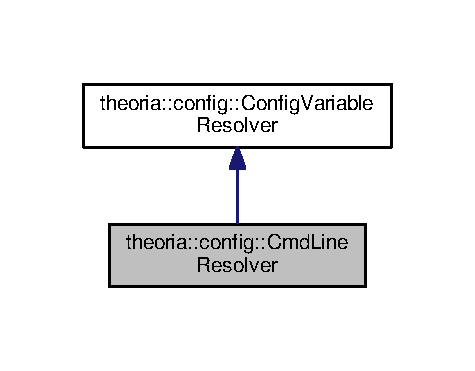
\includegraphics[width=228pt]{classtheoria_1_1config_1_1CmdLineResolver__inherit__graph}
\end{center}
\end{figure}


Collaboration diagram for theoria\+:\+:config\+:\+:Cmd\+Line\+Resolver\+:\nopagebreak
\begin{figure}[H]
\begin{center}
\leavevmode
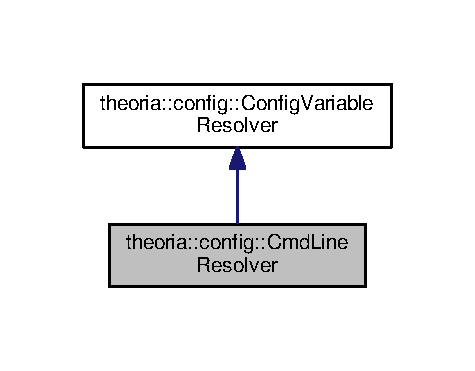
\includegraphics[width=228pt]{classtheoria_1_1config_1_1CmdLineResolver__coll__graph}
\end{center}
\end{figure}
\subsection*{Public Member Functions}
\begin{DoxyCompactItemize}
\item 
\hyperlink{classtheoria_1_1config_1_1ConfigVariableResolver_af27a85262d802c9ad4ecb1179efaf447}{Result} \hyperlink{classtheoria_1_1config_1_1CmdLineResolver_a6de270bd5855361b368cc082df53a527}{lookup} (const std\+::string \&\hyperlink{classtheoria_1_1config_1_1CmdLineResolver_ab42f0d86e62e985ee0bc94947df46a74}{name}) const override
\item 
virtual std\+::string \hyperlink{classtheoria_1_1config_1_1CmdLineResolver_ab42f0d86e62e985ee0bc94947df46a74}{name} () const override
\end{DoxyCompactItemize}
\subsection*{Additional Inherited Members}


\subsection{Detailed Description}
Resolves variables set from the theroia command line 

\subsection{Member Function Documentation}
\mbox{\Hypertarget{classtheoria_1_1config_1_1CmdLineResolver_a6de270bd5855361b368cc082df53a527}\label{classtheoria_1_1config_1_1CmdLineResolver_a6de270bd5855361b368cc082df53a527}} 
\index{theoria\+::config\+::\+Cmd\+Line\+Resolver@{theoria\+::config\+::\+Cmd\+Line\+Resolver}!lookup@{lookup}}
\index{lookup@{lookup}!theoria\+::config\+::\+Cmd\+Line\+Resolver@{theoria\+::config\+::\+Cmd\+Line\+Resolver}}
\subsubsection{\texorpdfstring{lookup()}{lookup()}}
{\footnotesize\ttfamily \hyperlink{classtheoria_1_1config_1_1ConfigVariableResolver_af27a85262d802c9ad4ecb1179efaf447}{Result} Cmd\+Line\+Resolver\+::lookup (\begin{DoxyParamCaption}\item[{const std\+::string \&}]{name }\end{DoxyParamCaption}) const\hspace{0.3cm}{\ttfamily [override]}, {\ttfamily [virtual]}}

Look up name in command line variables 

Implements \hyperlink{classtheoria_1_1config_1_1ConfigVariableResolver}{theoria\+::config\+::\+Config\+Variable\+Resolver}.

\mbox{\Hypertarget{classtheoria_1_1config_1_1CmdLineResolver_ab42f0d86e62e985ee0bc94947df46a74}\label{classtheoria_1_1config_1_1CmdLineResolver_ab42f0d86e62e985ee0bc94947df46a74}} 
\index{theoria\+::config\+::\+Cmd\+Line\+Resolver@{theoria\+::config\+::\+Cmd\+Line\+Resolver}!name@{name}}
\index{name@{name}!theoria\+::config\+::\+Cmd\+Line\+Resolver@{theoria\+::config\+::\+Cmd\+Line\+Resolver}}
\subsubsection{\texorpdfstring{name()}{name()}}
{\footnotesize\ttfamily std\+::string Cmd\+Line\+Resolver\+::name (\begin{DoxyParamCaption}{ }\end{DoxyParamCaption}) const\hspace{0.3cm}{\ttfamily [override]}, {\ttfamily [virtual]}}

Return \char`\"{}\+Cmd\+Line\+Resolver\char`\"{} 

Implements \hyperlink{classtheoria_1_1config_1_1ConfigVariableResolver_a026bda729faf988eaef334a45ec92303}{theoria\+::config\+::\+Config\+Variable\+Resolver}.



The documentation for this class was generated from the following files\+:\begin{DoxyCompactItemize}
\item 
include/theoria/config/Resolve.\+h\item 
src/config/Resolve.\+cpp\end{DoxyCompactItemize}

\hypertarget{classtheoria_1_1core_1_1CmdLineResolverComp}{}\section{theoria\+:\+:core\+:\+:Cmd\+Line\+Resolver\+Comp Class Reference}
\label{classtheoria_1_1core_1_1CmdLineResolverComp}\index{theoria\+::core\+::\+Cmd\+Line\+Resolver\+Comp@{theoria\+::core\+::\+Cmd\+Line\+Resolver\+Comp}}


Inheritance diagram for theoria\+:\+:core\+:\+:Cmd\+Line\+Resolver\+Comp\+:
\nopagebreak
\begin{figure}[H]
\begin{center}
\leavevmode
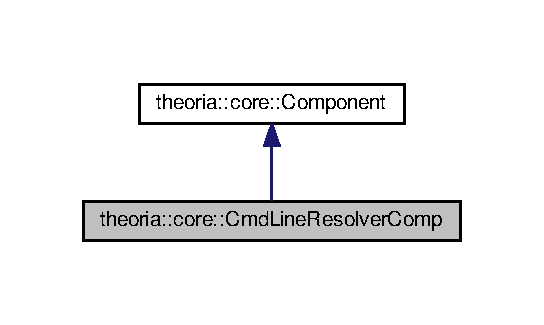
\includegraphics[width=261pt]{classtheoria_1_1core_1_1CmdLineResolverComp__inherit__graph}
\end{center}
\end{figure}


Collaboration diagram for theoria\+:\+:core\+:\+:Cmd\+Line\+Resolver\+Comp\+:
\nopagebreak
\begin{figure}[H]
\begin{center}
\leavevmode
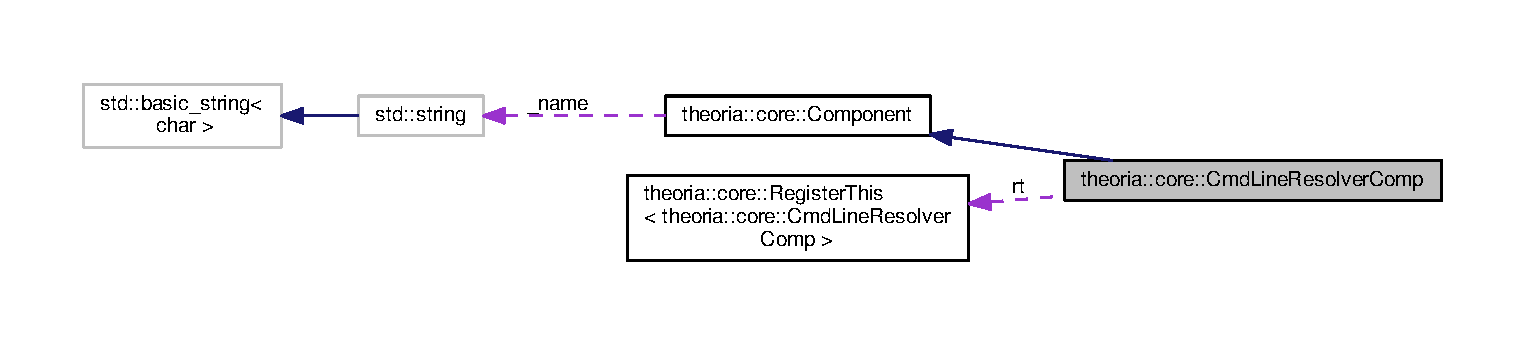
\includegraphics[width=350pt]{classtheoria_1_1core_1_1CmdLineResolverComp__coll__graph}
\end{center}
\end{figure}
\subsection*{Public Member Functions}
\begin{DoxyCompactItemize}
\item 
\mbox{\Hypertarget{classtheoria_1_1core_1_1CmdLineResolverComp_a4ed2c4896e0d20384e78c588f158c172}\label{classtheoria_1_1core_1_1CmdLineResolverComp_a4ed2c4896e0d20384e78c588f158c172}} 
{\bfseries Cmd\+Line\+Resolver\+Comp} (Comp\+Id id)
\item 
\mbox{\Hypertarget{classtheoria_1_1core_1_1CmdLineResolverComp_a51c66e964d559b3e13f4386c0bf0e0c0}\label{classtheoria_1_1core_1_1CmdLineResolverComp_a51c66e964d559b3e13f4386c0bf0e0c0}} 
\hyperlink{classtheoria_1_1core_1_1Component}{Component} $\ast$ {\bfseries acquire} (const std\+::type\+\_\+info \&type\+Info, void $\ast$$\ast$dest) override
\end{DoxyCompactItemize}
\subsection*{Static Public Member Functions}
\begin{DoxyCompactItemize}
\item 
\mbox{\Hypertarget{classtheoria_1_1core_1_1CmdLineResolverComp_a14fd80f330eb79fc13dcc25288c16bdf}\label{classtheoria_1_1core_1_1CmdLineResolverComp_a14fd80f330eb79fc13dcc25288c16bdf}} 
static \hyperlink{classtheoria_1_1core_1_1Component}{Component} $\ast$ {\bfseries factory} (Comp\+Id id)
\end{DoxyCompactItemize}
\subsection*{Static Public Attributes}
\begin{DoxyCompactItemize}
\item 
\mbox{\Hypertarget{classtheoria_1_1core_1_1CmdLineResolverComp_abcfcffaadb0282780e36034efc28f3aa}\label{classtheoria_1_1core_1_1CmdLineResolverComp_abcfcffaadb0282780e36034efc28f3aa}} 
static D\+L\+L\+\_\+\+P\+U\+B\+L\+IC \hyperlink{classtheoria_1_1core_1_1RegisterThis}{Register\+This}$<$ \hyperlink{classtheoria_1_1core_1_1CmdLineResolverComp}{Cmd\+Line\+Resolver\+Comp} $>$ {\bfseries rt}
\end{DoxyCompactItemize}
\subsection*{Additional Inherited Members}


The documentation for this class was generated from the following files\+:\begin{DoxyCompactItemize}
\item 
include/theoria/core/Core\+Components.\+h\item 
src/core/Core\+Components.\+cpp\end{DoxyCompactItemize}

\hypertarget{classtheoria_1_1util_1_1CommandLine}{}\section{theoria\+:\+:util\+:\+:Command\+Line Class Reference}
\label{classtheoria_1_1util_1_1CommandLine}\index{theoria\+::util\+::\+Command\+Line@{theoria\+::util\+::\+Command\+Line}}


{\ttfamily \#include $<$Command\+Line.\+h$>$}

\subsection*{Public Types}
\begin{DoxyCompactItemize}
\item 
using \hyperlink{classtheoria_1_1util_1_1CommandLine_a729aa00feedd8257d4caafc73ac6ee63}{const\+\_\+iterator} = Symbol\+Tbl\+::const\+\_\+iterator
\end{DoxyCompactItemize}
\subsection*{Public Member Functions}
\begin{DoxyCompactItemize}
\item 
\hyperlink{classtheoria_1_1util_1_1CommandLine_a7e753aa91c5a0018a1bec3439839852d}{Command\+Line} (int argc, const char $\ast$argv\mbox{[}$\,$\mbox{]}, bool allow\+Missing\+Config=false)
\item 
\hyperlink{classtheoria_1_1util_1_1CommandLine_a729aa00feedd8257d4caafc73ac6ee63}{const\+\_\+iterator} \hyperlink{classtheoria_1_1util_1_1CommandLine_adedd9cbacd108ee1b5454570a200f497}{find\+Var} (const std\+::string \&var) const
\item 
bool \hyperlink{classtheoria_1_1util_1_1CommandLine_adb659582b2ce6b2ef9666562ac05bd5f}{has\+Variable} (const std\+::string \&var) const
\item 
\hyperlink{classtheoria_1_1util_1_1CommandLine_a729aa00feedd8257d4caafc73ac6ee63}{const\+\_\+iterator} \hyperlink{classtheoria_1_1util_1_1CommandLine_a65446583fe4fe7d3a9ae1ed4dd23185e}{begin\+Vars} () const
\item 
\hyperlink{classtheoria_1_1util_1_1CommandLine_a729aa00feedd8257d4caafc73ac6ee63}{const\+\_\+iterator} \hyperlink{classtheoria_1_1util_1_1CommandLine_add5993c46a68548f70a75b2eb9431558}{end\+Vars} () const
\item 
const char $\ast$ \hyperlink{classtheoria_1_1util_1_1CommandLine_a26dab1188ed94478a4eaaf1b9e1ed19e}{variable\+As\+Ptr} (const std\+::string \&name) const noexcept
\item 
const std\+::string \& \hyperlink{classtheoria_1_1util_1_1CommandLine_aa9310fbfe3b1397bb9288eee7aae4abc}{variable\+As\+Str} (const std\+::string \&name, const std\+::string \&def=\char`\"{}\char`\"{}) const
\item 
int64\+\_\+t \hyperlink{classtheoria_1_1util_1_1CommandLine_a182748d9cfb606cbf45ee7dc7e016a52}{variable\+As\+Int} (const std\+::string \&name, int64\+\_\+t def=0) const
\item 
double \hyperlink{classtheoria_1_1util_1_1CommandLine_a42fbe66f3bcf121ad631df39d09606ef}{variable\+As\+Dbl} (const std\+::string \&name, double def=0) const
\item 
bool \hyperlink{classtheoria_1_1util_1_1CommandLine_a6d4d9be7adcf9ac15a1e5469535e97e9}{variable\+As\+Bool} (const std\+::string \&name, bool def) const
\item 
int \hyperlink{classtheoria_1_1util_1_1CommandLine_abe3bbdaa5b4abb7bf86996304b451253}{num\+Vars} () const
\item 
\hyperlink{classtheoria_1_1util_1_1CommandLine_a729aa00feedd8257d4caafc73ac6ee63}{const\+\_\+iterator} \hyperlink{classtheoria_1_1util_1_1CommandLine_abb86432416368ace970920f3fc4fe9c6}{find\+Setting} (const std\+::string \&name) const
\item 
bool \hyperlink{classtheoria_1_1util_1_1CommandLine_a011dfbb3035341128a4e4e4f4a466cff}{has\+Setting} (const std\+::string \&name) const
\item 
\hyperlink{classtheoria_1_1util_1_1CommandLine_a729aa00feedd8257d4caafc73ac6ee63}{const\+\_\+iterator} \hyperlink{classtheoria_1_1util_1_1CommandLine_ae0758c3259074eddfc06c4a77ac3a1a9}{begin\+Settings} () const
\item 
\hyperlink{classtheoria_1_1util_1_1CommandLine_a729aa00feedd8257d4caafc73ac6ee63}{const\+\_\+iterator} \hyperlink{classtheoria_1_1util_1_1CommandLine_ae33c86c2a60d2470827b2206893c8f7b}{end\+Settings} () const
\item 
const char $\ast$ \hyperlink{classtheoria_1_1util_1_1CommandLine_ad5b4089e23a04d31c3edcf3d659ab8d9}{setting\+As\+Ptr} (const std\+::string \&name) const noexcept
\item 
const std\+::string \& \hyperlink{classtheoria_1_1util_1_1CommandLine_ac398ce852930a3974f9ed6a1c5255975}{setting\+As\+Str} (const std\+::string \&name, const std\+::string \&def) const
\item 
int64\+\_\+t \hyperlink{classtheoria_1_1util_1_1CommandLine_abec4516f24ea88f83f1cabb16157cf8f}{setting\+As\+Int} (const std\+::string \&name, int64\+\_\+t def) const
\item 
double \hyperlink{classtheoria_1_1util_1_1CommandLine_ae2ff2d5845f93ac135e9e4a1ff65b403}{setting\+As\+Dbl} (const std\+::string \&name, double def) const
\item 
bool \hyperlink{classtheoria_1_1util_1_1CommandLine_a745baeae69017e95c9c9cbe4633be2d6}{setting\+As\+Bool} (const std\+::string \&name, bool def) const
\item 
int \hyperlink{classtheoria_1_1util_1_1CommandLine_aa0f4075a16a8c490e5e27596534ca485}{num\+Settings} () const
\item 
const std\+::string \& \hyperlink{classtheoria_1_1util_1_1CommandLine_abac7c59a7bf3989959f0023455f3257e}{config\+Filename} () const
\end{DoxyCompactItemize}
\subsection*{Static Public Member Functions}
\begin{DoxyCompactItemize}
\item 
static const \hyperlink{classtheoria_1_1util_1_1CommandLine}{Command\+Line} \& \hyperlink{classtheoria_1_1util_1_1CommandLine_a361f672089b8bd3cb794645ee4629b72}{instance} ()
\item 
static void \hyperlink{classtheoria_1_1util_1_1CommandLine_a1a52772e7e3b17d0dd7aa099f28c4f1e}{reset} ()
\end{DoxyCompactItemize}


\subsection{Detailed Description}
Pseudo-\/\+Singleton that captures command line arguments of Theoria applications

\hyperlink{classtheoria_1_1util_1_1CommandLine}{Command\+Line} consists of\+: \begin{DoxyVerb} config file - e.g., myapp.toml
 settings passed as: [--setting value] or [--someFlag] 
 settings are terminated by optionak -- (mandatory if variables are specified)
 variables passed as: var1=value

 Settings are usually predefined by theoria to change its behavior in some way specified by: theoria --help.
 However, user defined settings are allowed. To avoid conflict with future extensions of theoria
 user-defined settings should contain at least one capital letter (as theoria built-in settings are always lowere case)


 Variables are typically user defined settings that parameterize the config file. 
 See <theoria::config::CmdLineResolver>
\end{DoxyVerb}


Example legal command lines\+: \begin{DoxyVerb} theoria config.toml
 theoria config.xml
 theoria config.toml --setting1
 theoria config.toml --setting1 97
 theoria config.toml --setting1 --setting2 17
 theoria config.toml --setting1 --setting2 17 --
 theoria config.toml -- a=1 b=2 c=3
 theoria config.toml --setting1 --setting2 17 -- a=1 b=2 c=3 d=[1,2,3,4]\end{DoxyVerb}
 

\subsection{Member Typedef Documentation}
\mbox{\Hypertarget{classtheoria_1_1util_1_1CommandLine_a729aa00feedd8257d4caafc73ac6ee63}\label{classtheoria_1_1util_1_1CommandLine_a729aa00feedd8257d4caafc73ac6ee63}} 
\index{theoria\+::util\+::\+Command\+Line@{theoria\+::util\+::\+Command\+Line}!const\+\_\+iterator@{const\+\_\+iterator}}
\index{const\+\_\+iterator@{const\+\_\+iterator}!theoria\+::util\+::\+Command\+Line@{theoria\+::util\+::\+Command\+Line}}
\subsubsection{\texorpdfstring{const\+\_\+iterator}{const\_iterator}}
{\footnotesize\ttfamily using \hyperlink{classtheoria_1_1util_1_1CommandLine_a729aa00feedd8257d4caafc73ac6ee63}{theoria\+::util\+::\+Command\+Line\+::const\+\_\+iterator} =  Symbol\+Tbl\+::const\+\_\+iterator}

The iterator type for settings and variables 

\subsection{Constructor \& Destructor Documentation}
\mbox{\Hypertarget{classtheoria_1_1util_1_1CommandLine_a7e753aa91c5a0018a1bec3439839852d}\label{classtheoria_1_1util_1_1CommandLine_a7e753aa91c5a0018a1bec3439839852d}} 
\index{theoria\+::util\+::\+Command\+Line@{theoria\+::util\+::\+Command\+Line}!Command\+Line@{Command\+Line}}
\index{Command\+Line@{Command\+Line}!theoria\+::util\+::\+Command\+Line@{theoria\+::util\+::\+Command\+Line}}
\subsubsection{\texorpdfstring{Command\+Line()}{CommandLine()}}
{\footnotesize\ttfamily Command\+Line\+::\+Command\+Line (\begin{DoxyParamCaption}\item[{int}]{argc,  }\item[{const char $\ast$}]{argv\mbox{[}$\,$\mbox{]},  }\item[{bool}]{allow\+Missing\+Config = {\ttfamily false} }\end{DoxyParamCaption})}

Constructor takes argc and argv form main() (with first arg dropped) to initialize the command line object. It does not validate the actual values but does check that they conform to the order expected by theoria 

\subsection{Member Function Documentation}
\mbox{\Hypertarget{classtheoria_1_1util_1_1CommandLine_ae0758c3259074eddfc06c4a77ac3a1a9}\label{classtheoria_1_1util_1_1CommandLine_ae0758c3259074eddfc06c4a77ac3a1a9}} 
\index{theoria\+::util\+::\+Command\+Line@{theoria\+::util\+::\+Command\+Line}!begin\+Settings@{begin\+Settings}}
\index{begin\+Settings@{begin\+Settings}!theoria\+::util\+::\+Command\+Line@{theoria\+::util\+::\+Command\+Line}}
\subsubsection{\texorpdfstring{begin\+Settings()}{beginSettings()}}
{\footnotesize\ttfamily \hyperlink{classtheoria_1_1util_1_1CommandLine_a729aa00feedd8257d4caafc73ac6ee63}{const\+\_\+iterator} theoria\+::util\+::\+Command\+Line\+::begin\+Settings (\begin{DoxyParamCaption}{ }\end{DoxyParamCaption}) const\hspace{0.3cm}{\ttfamily [inline]}}

Iterator to the first setting \mbox{\Hypertarget{classtheoria_1_1util_1_1CommandLine_a65446583fe4fe7d3a9ae1ed4dd23185e}\label{classtheoria_1_1util_1_1CommandLine_a65446583fe4fe7d3a9ae1ed4dd23185e}} 
\index{theoria\+::util\+::\+Command\+Line@{theoria\+::util\+::\+Command\+Line}!begin\+Vars@{begin\+Vars}}
\index{begin\+Vars@{begin\+Vars}!theoria\+::util\+::\+Command\+Line@{theoria\+::util\+::\+Command\+Line}}
\subsubsection{\texorpdfstring{begin\+Vars()}{beginVars()}}
{\footnotesize\ttfamily \hyperlink{classtheoria_1_1util_1_1CommandLine_a729aa00feedd8257d4caafc73ac6ee63}{const\+\_\+iterator} theoria\+::util\+::\+Command\+Line\+::begin\+Vars (\begin{DoxyParamCaption}{ }\end{DoxyParamCaption}) const\hspace{0.3cm}{\ttfamily [inline]}}

Iterate over all variables \begin{DoxyReturn}{Returns}
iterator to std\+::pair$<$name,value$>$ or end() 
\end{DoxyReturn}
\mbox{\Hypertarget{classtheoria_1_1util_1_1CommandLine_abac7c59a7bf3989959f0023455f3257e}\label{classtheoria_1_1util_1_1CommandLine_abac7c59a7bf3989959f0023455f3257e}} 
\index{theoria\+::util\+::\+Command\+Line@{theoria\+::util\+::\+Command\+Line}!config\+Filename@{config\+Filename}}
\index{config\+Filename@{config\+Filename}!theoria\+::util\+::\+Command\+Line@{theoria\+::util\+::\+Command\+Line}}
\subsubsection{\texorpdfstring{config\+Filename()}{configFilename()}}
{\footnotesize\ttfamily const std\+::string\& theoria\+::util\+::\+Command\+Line\+::config\+Filename (\begin{DoxyParamCaption}{ }\end{DoxyParamCaption}) const\hspace{0.3cm}{\ttfamily [inline]}}

The name of the app config file bassed on the command line \mbox{\Hypertarget{classtheoria_1_1util_1_1CommandLine_ae33c86c2a60d2470827b2206893c8f7b}\label{classtheoria_1_1util_1_1CommandLine_ae33c86c2a60d2470827b2206893c8f7b}} 
\index{theoria\+::util\+::\+Command\+Line@{theoria\+::util\+::\+Command\+Line}!end\+Settings@{end\+Settings}}
\index{end\+Settings@{end\+Settings}!theoria\+::util\+::\+Command\+Line@{theoria\+::util\+::\+Command\+Line}}
\subsubsection{\texorpdfstring{end\+Settings()}{endSettings()}}
{\footnotesize\ttfamily \hyperlink{classtheoria_1_1util_1_1CommandLine_a729aa00feedd8257d4caafc73ac6ee63}{const\+\_\+iterator} theoria\+::util\+::\+Command\+Line\+::end\+Settings (\begin{DoxyParamCaption}{ }\end{DoxyParamCaption}) const\hspace{0.3cm}{\ttfamily [inline]}}

End of settings \mbox{\Hypertarget{classtheoria_1_1util_1_1CommandLine_add5993c46a68548f70a75b2eb9431558}\label{classtheoria_1_1util_1_1CommandLine_add5993c46a68548f70a75b2eb9431558}} 
\index{theoria\+::util\+::\+Command\+Line@{theoria\+::util\+::\+Command\+Line}!end\+Vars@{end\+Vars}}
\index{end\+Vars@{end\+Vars}!theoria\+::util\+::\+Command\+Line@{theoria\+::util\+::\+Command\+Line}}
\subsubsection{\texorpdfstring{end\+Vars()}{endVars()}}
{\footnotesize\ttfamily \hyperlink{classtheoria_1_1util_1_1CommandLine_a729aa00feedd8257d4caafc73ac6ee63}{const\+\_\+iterator} theoria\+::util\+::\+Command\+Line\+::end\+Vars (\begin{DoxyParamCaption}{ }\end{DoxyParamCaption}) const\hspace{0.3cm}{\ttfamily [inline]}}

The end of variables iterator \mbox{\Hypertarget{classtheoria_1_1util_1_1CommandLine_abb86432416368ace970920f3fc4fe9c6}\label{classtheoria_1_1util_1_1CommandLine_abb86432416368ace970920f3fc4fe9c6}} 
\index{theoria\+::util\+::\+Command\+Line@{theoria\+::util\+::\+Command\+Line}!find\+Setting@{find\+Setting}}
\index{find\+Setting@{find\+Setting}!theoria\+::util\+::\+Command\+Line@{theoria\+::util\+::\+Command\+Line}}
\subsubsection{\texorpdfstring{find\+Setting()}{findSetting()}}
{\footnotesize\ttfamily \hyperlink{classtheoria_1_1util_1_1CommandLine_a729aa00feedd8257d4caafc73ac6ee63}{const\+\_\+iterator} theoria\+::util\+::\+Command\+Line\+::find\+Setting (\begin{DoxyParamCaption}\item[{const std\+::string \&}]{name }\end{DoxyParamCaption}) const\hspace{0.3cm}{\ttfamily [inline]}}

Iterator to the named setting if it exists otherwise \hyperlink{classtheoria_1_1util_1_1CommandLine_ae33c86c2a60d2470827b2206893c8f7b}{end\+Settings()} \mbox{\Hypertarget{classtheoria_1_1util_1_1CommandLine_adedd9cbacd108ee1b5454570a200f497}\label{classtheoria_1_1util_1_1CommandLine_adedd9cbacd108ee1b5454570a200f497}} 
\index{theoria\+::util\+::\+Command\+Line@{theoria\+::util\+::\+Command\+Line}!find\+Var@{find\+Var}}
\index{find\+Var@{find\+Var}!theoria\+::util\+::\+Command\+Line@{theoria\+::util\+::\+Command\+Line}}
\subsubsection{\texorpdfstring{find\+Var()}{findVar()}}
{\footnotesize\ttfamily \hyperlink{classtheoria_1_1util_1_1CommandLine_a729aa00feedd8257d4caafc73ac6ee63}{const\+\_\+iterator} theoria\+::util\+::\+Command\+Line\+::find\+Var (\begin{DoxyParamCaption}\item[{const std\+::string \&}]{var }\end{DoxyParamCaption}) const\hspace{0.3cm}{\ttfamily [inline]}}

Find var if it exists \begin{DoxyReturn}{Returns}
const\+\_\+iterator to std\+::pair$<$var,value$>$ else \hyperlink{classtheoria_1_1util_1_1CommandLine_add5993c46a68548f70a75b2eb9431558}{end\+Vars()} 
\end{DoxyReturn}
\mbox{\Hypertarget{classtheoria_1_1util_1_1CommandLine_a011dfbb3035341128a4e4e4f4a466cff}\label{classtheoria_1_1util_1_1CommandLine_a011dfbb3035341128a4e4e4f4a466cff}} 
\index{theoria\+::util\+::\+Command\+Line@{theoria\+::util\+::\+Command\+Line}!has\+Setting@{has\+Setting}}
\index{has\+Setting@{has\+Setting}!theoria\+::util\+::\+Command\+Line@{theoria\+::util\+::\+Command\+Line}}
\subsubsection{\texorpdfstring{has\+Setting()}{hasSetting()}}
{\footnotesize\ttfamily bool theoria\+::util\+::\+Command\+Line\+::has\+Setting (\begin{DoxyParamCaption}\item[{const std\+::string \&}]{name }\end{DoxyParamCaption}) const\hspace{0.3cm}{\ttfamily [inline]}}

True if a setting with specified name exists \mbox{\Hypertarget{classtheoria_1_1util_1_1CommandLine_adb659582b2ce6b2ef9666562ac05bd5f}\label{classtheoria_1_1util_1_1CommandLine_adb659582b2ce6b2ef9666562ac05bd5f}} 
\index{theoria\+::util\+::\+Command\+Line@{theoria\+::util\+::\+Command\+Line}!has\+Variable@{has\+Variable}}
\index{has\+Variable@{has\+Variable}!theoria\+::util\+::\+Command\+Line@{theoria\+::util\+::\+Command\+Line}}
\subsubsection{\texorpdfstring{has\+Variable()}{hasVariable()}}
{\footnotesize\ttfamily bool theoria\+::util\+::\+Command\+Line\+::has\+Variable (\begin{DoxyParamCaption}\item[{const std\+::string \&}]{var }\end{DoxyParamCaption}) const\hspace{0.3cm}{\ttfamily [inline]}}

Test if variable exists 
\begin{DoxyParams}{Parameters}
{\em var} & the variable \\
\hline
\end{DoxyParams}
\begin{DoxyReturn}{Returns}
true if exists 
\end{DoxyReturn}
\mbox{\Hypertarget{classtheoria_1_1util_1_1CommandLine_a361f672089b8bd3cb794645ee4629b72}\label{classtheoria_1_1util_1_1CommandLine_a361f672089b8bd3cb794645ee4629b72}} 
\index{theoria\+::util\+::\+Command\+Line@{theoria\+::util\+::\+Command\+Line}!instance@{instance}}
\index{instance@{instance}!theoria\+::util\+::\+Command\+Line@{theoria\+::util\+::\+Command\+Line}}
\subsubsection{\texorpdfstring{instance()}{instance()}}
{\footnotesize\ttfamily const \hyperlink{classtheoria_1_1util_1_1CommandLine}{Command\+Line} \& Command\+Line\+::instance (\begin{DoxyParamCaption}{ }\end{DoxyParamCaption})\hspace{0.3cm}{\ttfamily [static]}}

The instance constructed in main (or first instance) \mbox{\Hypertarget{classtheoria_1_1util_1_1CommandLine_aa0f4075a16a8c490e5e27596534ca485}\label{classtheoria_1_1util_1_1CommandLine_aa0f4075a16a8c490e5e27596534ca485}} 
\index{theoria\+::util\+::\+Command\+Line@{theoria\+::util\+::\+Command\+Line}!num\+Settings@{num\+Settings}}
\index{num\+Settings@{num\+Settings}!theoria\+::util\+::\+Command\+Line@{theoria\+::util\+::\+Command\+Line}}
\subsubsection{\texorpdfstring{num\+Settings()}{numSettings()}}
{\footnotesize\ttfamily int theoria\+::util\+::\+Command\+Line\+::num\+Settings (\begin{DoxyParamCaption}{ }\end{DoxyParamCaption}) const\hspace{0.3cm}{\ttfamily [inline]}}

The numbber of settings passed on the command line \mbox{\Hypertarget{classtheoria_1_1util_1_1CommandLine_abe3bbdaa5b4abb7bf86996304b451253}\label{classtheoria_1_1util_1_1CommandLine_abe3bbdaa5b4abb7bf86996304b451253}} 
\index{theoria\+::util\+::\+Command\+Line@{theoria\+::util\+::\+Command\+Line}!num\+Vars@{num\+Vars}}
\index{num\+Vars@{num\+Vars}!theoria\+::util\+::\+Command\+Line@{theoria\+::util\+::\+Command\+Line}}
\subsubsection{\texorpdfstring{num\+Vars()}{numVars()}}
{\footnotesize\ttfamily int theoria\+::util\+::\+Command\+Line\+::num\+Vars (\begin{DoxyParamCaption}{ }\end{DoxyParamCaption}) const\hspace{0.3cm}{\ttfamily [inline]}}

Return the number of variables \mbox{\Hypertarget{classtheoria_1_1util_1_1CommandLine_a1a52772e7e3b17d0dd7aa099f28c4f1e}\label{classtheoria_1_1util_1_1CommandLine_a1a52772e7e3b17d0dd7aa099f28c4f1e}} 
\index{theoria\+::util\+::\+Command\+Line@{theoria\+::util\+::\+Command\+Line}!reset@{reset}}
\index{reset@{reset}!theoria\+::util\+::\+Command\+Line@{theoria\+::util\+::\+Command\+Line}}
\subsubsection{\texorpdfstring{reset()}{reset()}}
{\footnotesize\ttfamily void Command\+Line\+::reset (\begin{DoxyParamCaption}{ }\end{DoxyParamCaption})\hspace{0.3cm}{\ttfamily [static]}}

Reset the first instance \mbox{\Hypertarget{classtheoria_1_1util_1_1CommandLine_a745baeae69017e95c9c9cbe4633be2d6}\label{classtheoria_1_1util_1_1CommandLine_a745baeae69017e95c9c9cbe4633be2d6}} 
\index{theoria\+::util\+::\+Command\+Line@{theoria\+::util\+::\+Command\+Line}!setting\+As\+Bool@{setting\+As\+Bool}}
\index{setting\+As\+Bool@{setting\+As\+Bool}!theoria\+::util\+::\+Command\+Line@{theoria\+::util\+::\+Command\+Line}}
\subsubsection{\texorpdfstring{setting\+As\+Bool()}{settingAsBool()}}
{\footnotesize\ttfamily bool Command\+Line\+::setting\+As\+Bool (\begin{DoxyParamCaption}\item[{const std\+::string \&}]{name,  }\item[{bool}]{def }\end{DoxyParamCaption}) const}

Return a setting as a bool if it exists otherwise return def \mbox{\Hypertarget{classtheoria_1_1util_1_1CommandLine_ae2ff2d5845f93ac135e9e4a1ff65b403}\label{classtheoria_1_1util_1_1CommandLine_ae2ff2d5845f93ac135e9e4a1ff65b403}} 
\index{theoria\+::util\+::\+Command\+Line@{theoria\+::util\+::\+Command\+Line}!setting\+As\+Dbl@{setting\+As\+Dbl}}
\index{setting\+As\+Dbl@{setting\+As\+Dbl}!theoria\+::util\+::\+Command\+Line@{theoria\+::util\+::\+Command\+Line}}
\subsubsection{\texorpdfstring{setting\+As\+Dbl()}{settingAsDbl()}}
{\footnotesize\ttfamily double Command\+Line\+::setting\+As\+Dbl (\begin{DoxyParamCaption}\item[{const std\+::string \&}]{name,  }\item[{double}]{def }\end{DoxyParamCaption}) const}

Return a setting as double if it exists otherwise return def \mbox{\Hypertarget{classtheoria_1_1util_1_1CommandLine_abec4516f24ea88f83f1cabb16157cf8f}\label{classtheoria_1_1util_1_1CommandLine_abec4516f24ea88f83f1cabb16157cf8f}} 
\index{theoria\+::util\+::\+Command\+Line@{theoria\+::util\+::\+Command\+Line}!setting\+As\+Int@{setting\+As\+Int}}
\index{setting\+As\+Int@{setting\+As\+Int}!theoria\+::util\+::\+Command\+Line@{theoria\+::util\+::\+Command\+Line}}
\subsubsection{\texorpdfstring{setting\+As\+Int()}{settingAsInt()}}
{\footnotesize\ttfamily int64\+\_\+t Command\+Line\+::setting\+As\+Int (\begin{DoxyParamCaption}\item[{const std\+::string \&}]{name,  }\item[{int64\+\_\+t}]{def }\end{DoxyParamCaption}) const}

Return a settting as a 64bit integer if it exists otherwise return def \mbox{\Hypertarget{classtheoria_1_1util_1_1CommandLine_ad5b4089e23a04d31c3edcf3d659ab8d9}\label{classtheoria_1_1util_1_1CommandLine_ad5b4089e23a04d31c3edcf3d659ab8d9}} 
\index{theoria\+::util\+::\+Command\+Line@{theoria\+::util\+::\+Command\+Line}!setting\+As\+Ptr@{setting\+As\+Ptr}}
\index{setting\+As\+Ptr@{setting\+As\+Ptr}!theoria\+::util\+::\+Command\+Line@{theoria\+::util\+::\+Command\+Line}}
\subsubsection{\texorpdfstring{setting\+As\+Ptr()}{settingAsPtr()}}
{\footnotesize\ttfamily const char $\ast$ Command\+Line\+::setting\+As\+Ptr (\begin{DoxyParamCaption}\item[{const std\+::string \&}]{name }\end{DoxyParamCaption}) const\hspace{0.3cm}{\ttfamily [noexcept]}}

Return a settting as a const char $\ast$ if it exists otherwise return nullptr \mbox{\Hypertarget{classtheoria_1_1util_1_1CommandLine_ac398ce852930a3974f9ed6a1c5255975}\label{classtheoria_1_1util_1_1CommandLine_ac398ce852930a3974f9ed6a1c5255975}} 
\index{theoria\+::util\+::\+Command\+Line@{theoria\+::util\+::\+Command\+Line}!setting\+As\+Str@{setting\+As\+Str}}
\index{setting\+As\+Str@{setting\+As\+Str}!theoria\+::util\+::\+Command\+Line@{theoria\+::util\+::\+Command\+Line}}
\subsubsection{\texorpdfstring{setting\+As\+Str()}{settingAsStr()}}
{\footnotesize\ttfamily const std\+::string \& Command\+Line\+::setting\+As\+Str (\begin{DoxyParamCaption}\item[{const std\+::string \&}]{name,  }\item[{const std\+::string \&}]{def }\end{DoxyParamCaption}) const}

Return a settting as a string if it exists otherwise return def \mbox{\Hypertarget{classtheoria_1_1util_1_1CommandLine_a6d4d9be7adcf9ac15a1e5469535e97e9}\label{classtheoria_1_1util_1_1CommandLine_a6d4d9be7adcf9ac15a1e5469535e97e9}} 
\index{theoria\+::util\+::\+Command\+Line@{theoria\+::util\+::\+Command\+Line}!variable\+As\+Bool@{variable\+As\+Bool}}
\index{variable\+As\+Bool@{variable\+As\+Bool}!theoria\+::util\+::\+Command\+Line@{theoria\+::util\+::\+Command\+Line}}
\subsubsection{\texorpdfstring{variable\+As\+Bool()}{variableAsBool()}}
{\footnotesize\ttfamily bool Command\+Line\+::variable\+As\+Bool (\begin{DoxyParamCaption}\item[{const std\+::string \&}]{name,  }\item[{bool}]{def }\end{DoxyParamCaption}) const}

Get variable value as bool \begin{DoxyReturn}{Returns}
value or def if not present 
\end{DoxyReturn}

\begin{DoxyExceptions}{Exceptions}
{\em std\+::runtime\+\_\+error} & if can\textquotesingle{}t convert to a bool \\
\hline
\end{DoxyExceptions}
\mbox{\Hypertarget{classtheoria_1_1util_1_1CommandLine_a42fbe66f3bcf121ad631df39d09606ef}\label{classtheoria_1_1util_1_1CommandLine_a42fbe66f3bcf121ad631df39d09606ef}} 
\index{theoria\+::util\+::\+Command\+Line@{theoria\+::util\+::\+Command\+Line}!variable\+As\+Dbl@{variable\+As\+Dbl}}
\index{variable\+As\+Dbl@{variable\+As\+Dbl}!theoria\+::util\+::\+Command\+Line@{theoria\+::util\+::\+Command\+Line}}
\subsubsection{\texorpdfstring{variable\+As\+Dbl()}{variableAsDbl()}}
{\footnotesize\ttfamily double Command\+Line\+::variable\+As\+Dbl (\begin{DoxyParamCaption}\item[{const std\+::string \&}]{name,  }\item[{double}]{def = {\ttfamily 0} }\end{DoxyParamCaption}) const}

Get variable value as double \begin{DoxyReturn}{Returns}
value or def if not present 
\end{DoxyReturn}

\begin{DoxyExceptions}{Exceptions}
{\em std\+::runtime\+\_\+error} & if can\textquotesingle{}t convert to a double \\
\hline
\end{DoxyExceptions}
\mbox{\Hypertarget{classtheoria_1_1util_1_1CommandLine_a182748d9cfb606cbf45ee7dc7e016a52}\label{classtheoria_1_1util_1_1CommandLine_a182748d9cfb606cbf45ee7dc7e016a52}} 
\index{theoria\+::util\+::\+Command\+Line@{theoria\+::util\+::\+Command\+Line}!variable\+As\+Int@{variable\+As\+Int}}
\index{variable\+As\+Int@{variable\+As\+Int}!theoria\+::util\+::\+Command\+Line@{theoria\+::util\+::\+Command\+Line}}
\subsubsection{\texorpdfstring{variable\+As\+Int()}{variableAsInt()}}
{\footnotesize\ttfamily int64\+\_\+t Command\+Line\+::variable\+As\+Int (\begin{DoxyParamCaption}\item[{const std\+::string \&}]{name,  }\item[{int64\+\_\+t}]{def = {\ttfamily 0} }\end{DoxyParamCaption}) const}

Get variable value as int64\+\_\+t \begin{DoxyReturn}{Returns}
value or def if not present 
\end{DoxyReturn}

\begin{DoxyExceptions}{Exceptions}
{\em std\+::runtime\+\_\+error} & if can\textquotesingle{}t convert to an integer \\
\hline
\end{DoxyExceptions}
\mbox{\Hypertarget{classtheoria_1_1util_1_1CommandLine_a26dab1188ed94478a4eaaf1b9e1ed19e}\label{classtheoria_1_1util_1_1CommandLine_a26dab1188ed94478a4eaaf1b9e1ed19e}} 
\index{theoria\+::util\+::\+Command\+Line@{theoria\+::util\+::\+Command\+Line}!variable\+As\+Ptr@{variable\+As\+Ptr}}
\index{variable\+As\+Ptr@{variable\+As\+Ptr}!theoria\+::util\+::\+Command\+Line@{theoria\+::util\+::\+Command\+Line}}
\subsubsection{\texorpdfstring{variable\+As\+Ptr()}{variableAsPtr()}}
{\footnotesize\ttfamily const char $\ast$ Command\+Line\+::variable\+As\+Ptr (\begin{DoxyParamCaption}\item[{const std\+::string \&}]{name }\end{DoxyParamCaption}) const\hspace{0.3cm}{\ttfamily [noexcept]}}

Get variable value or nullptr as const char $\ast$ \begin{DoxyReturn}{Returns}
value or nullptr if not present 
\end{DoxyReturn}
\mbox{\Hypertarget{classtheoria_1_1util_1_1CommandLine_aa9310fbfe3b1397bb9288eee7aae4abc}\label{classtheoria_1_1util_1_1CommandLine_aa9310fbfe3b1397bb9288eee7aae4abc}} 
\index{theoria\+::util\+::\+Command\+Line@{theoria\+::util\+::\+Command\+Line}!variable\+As\+Str@{variable\+As\+Str}}
\index{variable\+As\+Str@{variable\+As\+Str}!theoria\+::util\+::\+Command\+Line@{theoria\+::util\+::\+Command\+Line}}
\subsubsection{\texorpdfstring{variable\+As\+Str()}{variableAsStr()}}
{\footnotesize\ttfamily const std\+::string \& Command\+Line\+::variable\+As\+Str (\begin{DoxyParamCaption}\item[{const std\+::string \&}]{name,  }\item[{const std\+::string \&}]{def = {\ttfamily \char`\"{}\char`\"{}} }\end{DoxyParamCaption}) const}

Get variable value as std\+::string \begin{DoxyReturn}{Returns}
value or def if not present 
\end{DoxyReturn}


The documentation for this class was generated from the following files\+:\begin{DoxyCompactItemize}
\item 
include/theoria/util/Command\+Line.\+h\item 
src/util/Command\+Line.\+cpp\end{DoxyCompactItemize}

\hypertarget{classtheoria_1_1core_1_1Component}{}\section{theoria\+:\+:core\+:\+:Component Class Reference}
\label{classtheoria_1_1core_1_1Component}\index{theoria\+::core\+::\+Component@{theoria\+::core\+::\+Component}}


{\ttfamily \#include $<$Component.\+h$>$}



Inheritance diagram for theoria\+:\+:core\+:\+:Component\+:\nopagebreak
\begin{figure}[H]
\begin{center}
\leavevmode
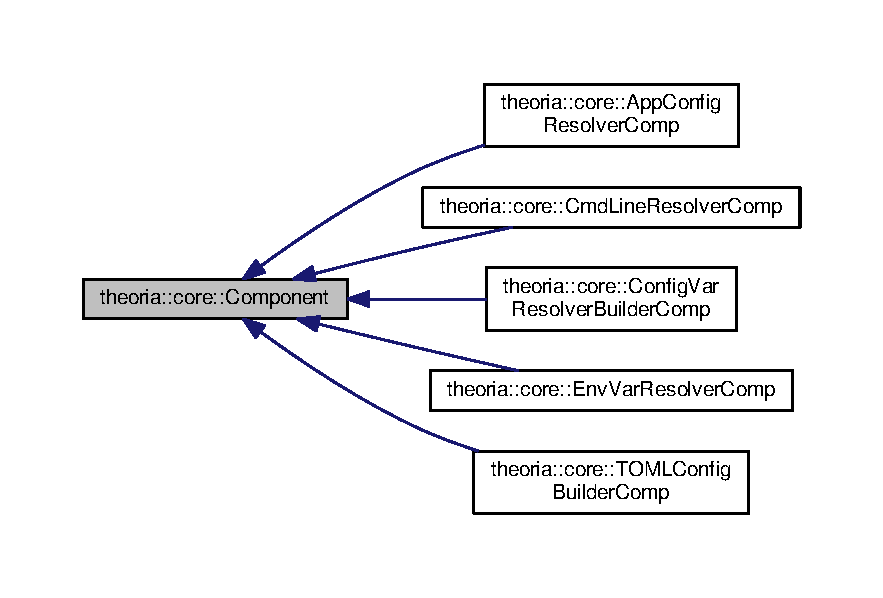
\includegraphics[width=350pt]{classtheoria_1_1core_1_1Component__inherit__graph}
\end{center}
\end{figure}


Collaboration diagram for theoria\+:\+:core\+:\+:Component\+:\nopagebreak
\begin{figure}[H]
\begin{center}
\leavevmode
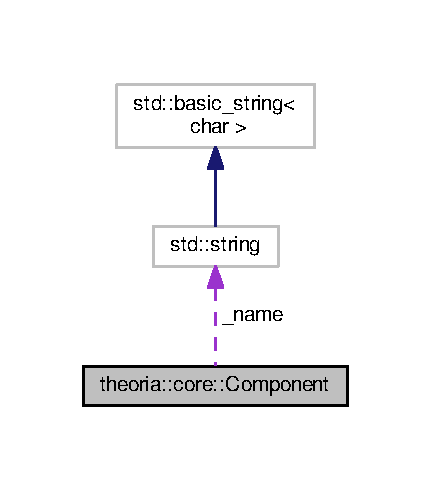
\includegraphics[width=207pt]{classtheoria_1_1core_1_1Component__coll__graph}
\end{center}
\end{figure}
\subsection*{Public Member Functions}
\begin{DoxyCompactItemize}
\item 
\hyperlink{classtheoria_1_1core_1_1Component_a8775db6d1a2c1afc2e77cd3c8f39da6f}{Component} ()
\item 
\hyperlink{classtheoria_1_1core_1_1Component_a64b1e60585ad8c0d12d9be814b37dda8}{Component} (Comp\+Id \hyperlink{classtheoria_1_1core_1_1Component_ab539df9f996efceda7743fa1b69cd25d}{id})
\item 
\hyperlink{classtheoria_1_1core_1_1Component_a719767a45a12a3d12670aadd83f5d292}{Component} (Comp\+Id \hyperlink{classtheoria_1_1core_1_1Component_ab539df9f996efceda7743fa1b69cd25d}{id}, const std\+::string \&\hyperlink{classtheoria_1_1core_1_1Component_ae0a32f194c007fe419ec9ae9303025fc}{name})
\item 
virtual \hyperlink{classtheoria_1_1core_1_1Component_ab8378fa275af98e568a7e91d33d867af}{$\sim$\+Component} ()
\item 
virtual \hyperlink{classtheoria_1_1core_1_1Dependencies}{Dependencies} \hyperlink{classtheoria_1_1core_1_1Component_a7ed45f6e38442a40666ae4556f794f7d}{init} (const \hyperlink{classtheoria_1_1config_1_1Config}{config\+::\+Config} \&config)
\item 
virtual void \hyperlink{classtheoria_1_1core_1_1Component_afd8acc89e2cd36e92bebe7e6fa530764}{finalize} (const std\+::vector$<$ \hyperlink{classtheoria_1_1core_1_1Component}{Component} $\ast$$>$ \&dependencies)
\item 
virtual void \hyperlink{classtheoria_1_1core_1_1Component_ae036cde9b803a621149efeff7e0e00fc}{app\+Life\+Cycle} (App\+Life\+Cycle state)
\item 
virtual void \hyperlink{classtheoria_1_1core_1_1Component_a92578e2b6253681a21b91e7c22b22975}{comp\+Life\+Cycle} (Comp\+Life\+Cycle state, Comp\+Id \hyperlink{classtheoria_1_1core_1_1Component_ab539df9f996efceda7743fa1b69cd25d}{id})
\item 
virtual void \hyperlink{classtheoria_1_1core_1_1Component_a6b6d003ecdddc3eee401917f01ae7a1d}{on\+Message} (const \hyperlink{classtheoria_1_1core_1_1Message}{Message} \&msg)
\item 
Comp\+Id \hyperlink{classtheoria_1_1core_1_1Component_ab539df9f996efceda7743fa1b69cd25d}{id} () const
\item 
const std\+::string \& \hyperlink{classtheoria_1_1core_1_1Component_ae0a32f194c007fe419ec9ae9303025fc}{name} () const
\item 
void \hyperlink{classtheoria_1_1core_1_1Component_a4c741f3d65b7d50bd56378bdc9cc9a62}{set\+Name} (const std\+::string \&\hyperlink{classtheoria_1_1core_1_1Component_ae0a32f194c007fe419ec9ae9303025fc}{name})
\item 
{\footnotesize template$<$class T $>$ }\\T $\ast$ \hyperlink{classtheoria_1_1core_1_1Component_a1b3e32c74b8a8bb6701918ec8114c606}{cast} (const std\+::string \&requestor=\char`\"{}Unknown\char`\"{})
\item 
virtual \hyperlink{classtheoria_1_1core_1_1Component}{Component} $\ast$ \hyperlink{classtheoria_1_1core_1_1Component_a18744abc83e088af3c3d42e0a22c35e3}{acquire} (const std\+::type\+\_\+info \&type\+Info, void $\ast$$\ast$dest)
\end{DoxyCompactItemize}
\subsection*{Protected Attributes}
\begin{DoxyCompactItemize}
\item 
Comp\+Id \hyperlink{classtheoria_1_1core_1_1Component_a460b08de1c87f984fe9b6e4a1b8b50e6}{\+\_\+id}
\item 
std\+::string \hyperlink{classtheoria_1_1core_1_1Component_ac1eca19b044721b873a0ec32cf3667a1}{\+\_\+name}
\end{DoxyCompactItemize}


\subsection{Detailed Description}
Components are the soul of \hyperlink{classtheoria_1_1core_1_1Theoria}{Theoria}. Components are used to implement the meaty parts of your application. Things that contain significant business logic, are generally long-\/lived, manage complex data structures, processes or algorithms, etc. Components support a rich lifecycle, can be dynamically configured and dynamically wired up to other components.

Components consume config data to customize themselves to a particular use. Config data is provided in the \hyperlink{classtheoria_1_1core_1_1Component_a7ed45f6e38442a40666ae4556f794f7d}{init()} method and it is the first stage of a components lifecycle. Often this cofiguration will provide information that will tell a component what other components it requires but other times the configuration data will be simple paramters like a host/port or locale info, or user settings, etc.

In response to configuraation a component is expected to return its requirements for other components. It does this by returning \hyperlink{classtheoria_1_1core_1_1Dependencies}{Dependencies}. \hyperlink{classtheoria_1_1core_1_1Dependencies}{Dependencies} are a way of conveying very general or very specific requirements that of this component to other components. A specific requirement is communicated as a Type and Subtype. Here we use Type to mean \char`\"{}the need of a component that provides some service\char`\"{} and Subtype to mean a very specific implematation of that service. In addition, \hyperlink{classtheoria_1_1core_1_1Dependencies}{Dependencies} convey whether a service is absolutly required or is optional. An absolute requirement must be fullfiled for the application to progress.

Once all components in you application are initialized, \hyperlink{classtheoria_1_1core_1_1Theoria}{Theoria} satisfies dependencies by calling \hyperlink{classtheoria_1_1core_1_1Component_afd8acc89e2cd36e92bebe7e6fa530764}{finalize()} and handing your componet its dependents in the same order as requested. Optional dependents may be null if \hyperlink{classtheoria_1_1core_1_1Theoria}{Theoria} could not aquire them

Components also receive life-\/cycle notifications. \begin{DoxySeeAlso}{See also}
\hyperlink{classtheoria_1_1core_1_1Component_ae036cde9b803a621149efeff7e0e00fc}{app\+Life\+Cycle} and 

\hyperlink{classtheoria_1_1core_1_1Component_a92578e2b6253681a21b91e7c22b22975}{comp\+Life\+Cycle} for details. 
\end{DoxySeeAlso}


\subsection{Constructor \& Destructor Documentation}
\mbox{\Hypertarget{classtheoria_1_1core_1_1Component_a8775db6d1a2c1afc2e77cd3c8f39da6f}\label{classtheoria_1_1core_1_1Component_a8775db6d1a2c1afc2e77cd3c8f39da6f}} 
\index{theoria\+::core\+::\+Component@{theoria\+::core\+::\+Component}!Component@{Component}}
\index{Component@{Component}!theoria\+::core\+::\+Component@{theoria\+::core\+::\+Component}}
\subsubsection{\texorpdfstring{Component()}{Component()}\hspace{0.1cm}{\footnotesize\ttfamily [1/3]}}
{\footnotesize\ttfamily Component\+::\+Component (\begin{DoxyParamCaption}{ }\end{DoxyParamCaption})}

Empty component \mbox{\Hypertarget{classtheoria_1_1core_1_1Component_a64b1e60585ad8c0d12d9be814b37dda8}\label{classtheoria_1_1core_1_1Component_a64b1e60585ad8c0d12d9be814b37dda8}} 
\index{theoria\+::core\+::\+Component@{theoria\+::core\+::\+Component}!Component@{Component}}
\index{Component@{Component}!theoria\+::core\+::\+Component@{theoria\+::core\+::\+Component}}
\subsubsection{\texorpdfstring{Component()}{Component()}\hspace{0.1cm}{\footnotesize\ttfamily [2/3]}}
{\footnotesize\ttfamily theoria\+::core\+::\+Component\+::\+Component (\begin{DoxyParamCaption}\item[{Comp\+Id}]{id }\end{DoxyParamCaption})\hspace{0.3cm}{\ttfamily [inline]}}

Construct component with specified id \mbox{\Hypertarget{classtheoria_1_1core_1_1Component_a719767a45a12a3d12670aadd83f5d292}\label{classtheoria_1_1core_1_1Component_a719767a45a12a3d12670aadd83f5d292}} 
\index{theoria\+::core\+::\+Component@{theoria\+::core\+::\+Component}!Component@{Component}}
\index{Component@{Component}!theoria\+::core\+::\+Component@{theoria\+::core\+::\+Component}}
\subsubsection{\texorpdfstring{Component()}{Component()}\hspace{0.1cm}{\footnotesize\ttfamily [3/3]}}
{\footnotesize\ttfamily theoria\+::core\+::\+Component\+::\+Component (\begin{DoxyParamCaption}\item[{Comp\+Id}]{id,  }\item[{const std\+::string \&}]{name }\end{DoxyParamCaption})\hspace{0.3cm}{\ttfamily [inline]}}

Construct component with specified id and name \mbox{\Hypertarget{classtheoria_1_1core_1_1Component_ab8378fa275af98e568a7e91d33d867af}\label{classtheoria_1_1core_1_1Component_ab8378fa275af98e568a7e91d33d867af}} 
\index{theoria\+::core\+::\+Component@{theoria\+::core\+::\+Component}!````~Component@{$\sim$\+Component}}
\index{````~Component@{$\sim$\+Component}!theoria\+::core\+::\+Component@{theoria\+::core\+::\+Component}}
\subsubsection{\texorpdfstring{$\sim$\+Component()}{~Component()}}
{\footnotesize\ttfamily Component\+::$\sim$\+Component (\begin{DoxyParamCaption}{ }\end{DoxyParamCaption})\hspace{0.3cm}{\ttfamily [virtual]}}

Destructor 

\subsection{Member Function Documentation}
\mbox{\Hypertarget{classtheoria_1_1core_1_1Component_a18744abc83e088af3c3d42e0a22c35e3}\label{classtheoria_1_1core_1_1Component_a18744abc83e088af3c3d42e0a22c35e3}} 
\index{theoria\+::core\+::\+Component@{theoria\+::core\+::\+Component}!acquire@{acquire}}
\index{acquire@{acquire}!theoria\+::core\+::\+Component@{theoria\+::core\+::\+Component}}
\subsubsection{\texorpdfstring{acquire()}{acquire()}}
{\footnotesize\ttfamily \hyperlink{classtheoria_1_1core_1_1Component}{Component} $\ast$ Component\+::acquire (\begin{DoxyParamCaption}\item[{const std\+::type\+\_\+info \&}]{type\+Info,  }\item[{void $\ast$$\ast$}]{dest }\end{DoxyParamCaption})\hspace{0.3cm}{\ttfamily [virtual]}}

Override in your component if you want to control how other components acquire interfaces from you. Your are responsible for using the type\+Info to return a suitable object in destination. If you can\textquotesingle{}t do this you can optionally return another \hyperlink{classtheoria_1_1core_1_1Component}{Component} that you think can.

Default impl sets $\ast$dest to nullptr and returns nullptr


\begin{DoxyParams}{Parameters}
{\em type\+Info} & the type\+\_\+info of he type you wish to acquire \\
\hline
{\em dest} & the dest where a pointer to the impl of type\+\_\+info will be stored if available \\
\hline
\end{DoxyParams}
\begin{DoxyReturn}{Returns}
nullptr if this call already satisfied the request by populating dest or if it can\textquotesingle{}t satify request a pointer to another component if this component belives that the returned component can satisfy the request 
\end{DoxyReturn}


Reimplemented in \hyperlink{classtheoria_1_1core_1_1TOMLConfigBuilderComp_a7cfce41f96c49af8e80d884f70ee66fa}{theoria\+::core\+::\+T\+O\+M\+L\+Config\+Builder\+Comp}, \hyperlink{classtheoria_1_1core_1_1AppConfigResolverComp_af04af67f66e3bfea44ab76c33d64a51e}{theoria\+::core\+::\+App\+Config\+Resolver\+Comp}, \hyperlink{classtheoria_1_1core_1_1CmdLineResolverComp_a51c66e964d559b3e13f4386c0bf0e0c0}{theoria\+::core\+::\+Cmd\+Line\+Resolver\+Comp}, and \hyperlink{classtheoria_1_1core_1_1EnvVarResolverComp_aac22e843f14123d2627f8c8ca0311b80}{theoria\+::core\+::\+Env\+Var\+Resolver\+Comp}.

\mbox{\Hypertarget{classtheoria_1_1core_1_1Component_ae036cde9b803a621149efeff7e0e00fc}\label{classtheoria_1_1core_1_1Component_ae036cde9b803a621149efeff7e0e00fc}} 
\index{theoria\+::core\+::\+Component@{theoria\+::core\+::\+Component}!app\+Life\+Cycle@{app\+Life\+Cycle}}
\index{app\+Life\+Cycle@{app\+Life\+Cycle}!theoria\+::core\+::\+Component@{theoria\+::core\+::\+Component}}
\subsubsection{\texorpdfstring{app\+Life\+Cycle()}{appLifeCycle()}}
{\footnotesize\ttfamily void Component\+::app\+Life\+Cycle (\begin{DoxyParamCaption}\item[{App\+Life\+Cycle}]{state }\end{DoxyParamCaption})\hspace{0.3cm}{\ttfamily [virtual]}}

This is a place to take action on application lifecycle events. 

Reimplemented in \hyperlink{classtheoria_1_1core_1_1ConfigVarResolverBuilderComp_ad7d3e9f8ab3a2837526ffc3eda4c6c38}{theoria\+::core\+::\+Config\+Var\+Resolver\+Builder\+Comp}.

\mbox{\Hypertarget{classtheoria_1_1core_1_1Component_a1b3e32c74b8a8bb6701918ec8114c606}\label{classtheoria_1_1core_1_1Component_a1b3e32c74b8a8bb6701918ec8114c606}} 
\index{theoria\+::core\+::\+Component@{theoria\+::core\+::\+Component}!cast@{cast}}
\index{cast@{cast}!theoria\+::core\+::\+Component@{theoria\+::core\+::\+Component}}
\subsubsection{\texorpdfstring{cast()}{cast()}}
{\footnotesize\ttfamily template$<$class T $>$ \\
T$\ast$ theoria\+::core\+::\+Component\+::cast (\begin{DoxyParamCaption}\item[{const std\+::string \&}]{requestor = {\ttfamily \char`\"{}Unknown\char`\"{}} }\end{DoxyParamCaption})\hspace{0.3cm}{\ttfamily [inline]}}

A cast operation is a request to this component for an implemetation of type T. The component can satisfy the request if it is itself a T or if it can acquire a T. \begin{DoxySeeAlso}{See also}
\hyperlink{classtheoria_1_1core_1_1Component_a18744abc83e088af3c3d42e0a22c35e3}{acquire} 
\end{DoxySeeAlso}
\mbox{\Hypertarget{classtheoria_1_1core_1_1Component_a92578e2b6253681a21b91e7c22b22975}\label{classtheoria_1_1core_1_1Component_a92578e2b6253681a21b91e7c22b22975}} 
\index{theoria\+::core\+::\+Component@{theoria\+::core\+::\+Component}!comp\+Life\+Cycle@{comp\+Life\+Cycle}}
\index{comp\+Life\+Cycle@{comp\+Life\+Cycle}!theoria\+::core\+::\+Component@{theoria\+::core\+::\+Component}}
\subsubsection{\texorpdfstring{comp\+Life\+Cycle()}{compLifeCycle()}}
{\footnotesize\ttfamily void Component\+::comp\+Life\+Cycle (\begin{DoxyParamCaption}\item[{Comp\+Life\+Cycle}]{state,  }\item[{Comp\+Id}]{id }\end{DoxyParamCaption})\hspace{0.3cm}{\ttfamily [virtual]}}

This is a place to take action on events related to components you depend on \mbox{\Hypertarget{classtheoria_1_1core_1_1Component_afd8acc89e2cd36e92bebe7e6fa530764}\label{classtheoria_1_1core_1_1Component_afd8acc89e2cd36e92bebe7e6fa530764}} 
\index{theoria\+::core\+::\+Component@{theoria\+::core\+::\+Component}!finalize@{finalize}}
\index{finalize@{finalize}!theoria\+::core\+::\+Component@{theoria\+::core\+::\+Component}}
\subsubsection{\texorpdfstring{finalize()}{finalize()}}
{\footnotesize\ttfamily void Component\+::finalize (\begin{DoxyParamCaption}\item[{const std\+::vector$<$ \hyperlink{classtheoria_1_1core_1_1Component}{Component} $\ast$$>$ \&}]{dependencies }\end{DoxyParamCaption})\hspace{0.3cm}{\ttfamily [virtual]}}

Receive the components you required in \hyperlink{classtheoria_1_1core_1_1Component_a7ed45f6e38442a40666ae4556f794f7d}{init()}. Optional components will be nullptrs. All components received are initialized but not necessarily finalized so do not call into the component yet (unless you really know what you are doing but you are prob asking for trouble) 

Reimplemented in \hyperlink{classtheoria_1_1core_1_1ConfigVarResolverBuilderComp_ac1e585a908c7e0fa7db4bdf0a8b514bb}{theoria\+::core\+::\+Config\+Var\+Resolver\+Builder\+Comp}.

\mbox{\Hypertarget{classtheoria_1_1core_1_1Component_ab539df9f996efceda7743fa1b69cd25d}\label{classtheoria_1_1core_1_1Component_ab539df9f996efceda7743fa1b69cd25d}} 
\index{theoria\+::core\+::\+Component@{theoria\+::core\+::\+Component}!id@{id}}
\index{id@{id}!theoria\+::core\+::\+Component@{theoria\+::core\+::\+Component}}
\subsubsection{\texorpdfstring{id()}{id()}}
{\footnotesize\ttfamily Comp\+Id theoria\+::core\+::\+Component\+::id (\begin{DoxyParamCaption}{ }\end{DoxyParamCaption}) const\hspace{0.3cm}{\ttfamily [inline]}}

Return components unique id. Uniquieness is per application invocation so this is not a G\+U\+ID nor is it guranteed idemponent between distinct runs of the app. \mbox{\Hypertarget{classtheoria_1_1core_1_1Component_a7ed45f6e38442a40666ae4556f794f7d}\label{classtheoria_1_1core_1_1Component_a7ed45f6e38442a40666ae4556f794f7d}} 
\index{theoria\+::core\+::\+Component@{theoria\+::core\+::\+Component}!init@{init}}
\index{init@{init}!theoria\+::core\+::\+Component@{theoria\+::core\+::\+Component}}
\subsubsection{\texorpdfstring{init()}{init()}}
{\footnotesize\ttfamily \hyperlink{classtheoria_1_1core_1_1Dependencies}{Dependencies} Component\+::init (\begin{DoxyParamCaption}\item[{const \hyperlink{classtheoria_1_1config_1_1Config}{config\+::\+Config} \&}]{config }\end{DoxyParamCaption})\hspace{0.3cm}{\ttfamily [virtual]}}

Initialize component from its configuration and return the Components dependencies 

Reimplemented in \hyperlink{classtheoria_1_1core_1_1ConfigVarResolverBuilderComp_aadf94c8b3d765667eaf9d7c91ac65342}{theoria\+::core\+::\+Config\+Var\+Resolver\+Builder\+Comp}.

\mbox{\Hypertarget{classtheoria_1_1core_1_1Component_ae0a32f194c007fe419ec9ae9303025fc}\label{classtheoria_1_1core_1_1Component_ae0a32f194c007fe419ec9ae9303025fc}} 
\index{theoria\+::core\+::\+Component@{theoria\+::core\+::\+Component}!name@{name}}
\index{name@{name}!theoria\+::core\+::\+Component@{theoria\+::core\+::\+Component}}
\subsubsection{\texorpdfstring{name()}{name()}}
{\footnotesize\ttfamily const std\+::string\& theoria\+::core\+::\+Component\+::name (\begin{DoxyParamCaption}{ }\end{DoxyParamCaption}) const\hspace{0.3cm}{\ttfamily [inline]}}

The component\textquotesingle{}s name (usually from configuration) \mbox{\Hypertarget{classtheoria_1_1core_1_1Component_a6b6d003ecdddc3eee401917f01ae7a1d}\label{classtheoria_1_1core_1_1Component_a6b6d003ecdddc3eee401917f01ae7a1d}} 
\index{theoria\+::core\+::\+Component@{theoria\+::core\+::\+Component}!on\+Message@{on\+Message}}
\index{on\+Message@{on\+Message}!theoria\+::core\+::\+Component@{theoria\+::core\+::\+Component}}
\subsubsection{\texorpdfstring{on\+Message()}{onMessage()}}
{\footnotesize\ttfamily void Component\+::on\+Message (\begin{DoxyParamCaption}\item[{const \hyperlink{classtheoria_1_1core_1_1Message}{Message} \&}]{msg }\end{DoxyParamCaption})\hspace{0.3cm}{\ttfamily [virtual]}}

If your coponent is a member of a event loop, async messages arrive here \mbox{\Hypertarget{classtheoria_1_1core_1_1Component_a4c741f3d65b7d50bd56378bdc9cc9a62}\label{classtheoria_1_1core_1_1Component_a4c741f3d65b7d50bd56378bdc9cc9a62}} 
\index{theoria\+::core\+::\+Component@{theoria\+::core\+::\+Component}!set\+Name@{set\+Name}}
\index{set\+Name@{set\+Name}!theoria\+::core\+::\+Component@{theoria\+::core\+::\+Component}}
\subsubsection{\texorpdfstring{set\+Name()}{setName()}}
{\footnotesize\ttfamily void theoria\+::core\+::\+Component\+::set\+Name (\begin{DoxyParamCaption}\item[{const std\+::string \&}]{name }\end{DoxyParamCaption})\hspace{0.3cm}{\ttfamily [inline]}}

Set or change the components name 

\subsection{Member Data Documentation}
\mbox{\Hypertarget{classtheoria_1_1core_1_1Component_a460b08de1c87f984fe9b6e4a1b8b50e6}\label{classtheoria_1_1core_1_1Component_a460b08de1c87f984fe9b6e4a1b8b50e6}} 
\index{theoria\+::core\+::\+Component@{theoria\+::core\+::\+Component}!\+\_\+id@{\+\_\+id}}
\index{\+\_\+id@{\+\_\+id}!theoria\+::core\+::\+Component@{theoria\+::core\+::\+Component}}
\subsubsection{\texorpdfstring{\+\_\+id}{\_id}}
{\footnotesize\ttfamily Comp\+Id theoria\+::core\+::\+Component\+::\+\_\+id\hspace{0.3cm}{\ttfamily [protected]}}

Unique id \mbox{\Hypertarget{classtheoria_1_1core_1_1Component_ac1eca19b044721b873a0ec32cf3667a1}\label{classtheoria_1_1core_1_1Component_ac1eca19b044721b873a0ec32cf3667a1}} 
\index{theoria\+::core\+::\+Component@{theoria\+::core\+::\+Component}!\+\_\+name@{\+\_\+name}}
\index{\+\_\+name@{\+\_\+name}!theoria\+::core\+::\+Component@{theoria\+::core\+::\+Component}}
\subsubsection{\texorpdfstring{\+\_\+name}{\_name}}
{\footnotesize\ttfamily std\+::string theoria\+::core\+::\+Component\+::\+\_\+name\hspace{0.3cm}{\ttfamily [protected]}}

Name 

The documentation for this class was generated from the following files\+:\begin{DoxyCompactItemize}
\item 
include/theoria/core/Component.\+h\item 
src/core/Component.\+cpp\end{DoxyCompactItemize}

\hypertarget{classtheoria_1_1core_1_1ComponentData}{\section{theoria\+:\+:core\+:\+:Component\+Data Class Reference}
\label{classtheoria_1_1core_1_1ComponentData}\index{theoria\+::core\+::\+Component\+Data@{theoria\+::core\+::\+Component\+Data}}
}
\subsection*{Public Types}
\begin{DoxyCompactItemize}
\item 
\hypertarget{classtheoria_1_1core_1_1ComponentData_a66b4a86a617891cfd780d447c82b88b0}{using {\bfseries baseid\+\_\+const\+\_\+iterator} = Base\+List\+::const\+\_\+iterator}\label{classtheoria_1_1core_1_1ComponentData_a66b4a86a617891cfd780d447c82b88b0}

\end{DoxyCompactItemize}
\subsection*{Public Member Functions}
\begin{DoxyCompactItemize}
\item 
\hypertarget{classtheoria_1_1core_1_1ComponentData_a93362592e0c3f5e624e06cca44f3b451}{baseid\+\_\+const\+\_\+iterator {\bfseries begin\+Base\+Id} () const }\label{classtheoria_1_1core_1_1ComponentData_a93362592e0c3f5e624e06cca44f3b451}

\item 
\hypertarget{classtheoria_1_1core_1_1ComponentData_a177b871167661709317659aaa2229ee1}{baseid\+\_\+const\+\_\+iterator {\bfseries end\+Base\+Id} () const }\label{classtheoria_1_1core_1_1ComponentData_a177b871167661709317659aaa2229ee1}

\item 
\hypertarget{classtheoria_1_1core_1_1ComponentData_ae2b0bd7575fb44f9e75b70f07f71fb59}{Comp\+Id {\bfseries id} () const }\label{classtheoria_1_1core_1_1ComponentData_ae2b0bd7575fb44f9e75b70f07f71fb59}

\item 
\hypertarget{classtheoria_1_1core_1_1ComponentData_a577f3f27a672f1b9e9bfb32a4798a44b}{Type\+Name {\bfseries type} () const }\label{classtheoria_1_1core_1_1ComponentData_a577f3f27a672f1b9e9bfb32a4798a44b}

\item 
\hypertarget{classtheoria_1_1core_1_1ComponentData_affc0a5651ebe40065a90cc509ebbfd26}{Type\+Name\+List {\bfseries base\+Types} () const }\label{classtheoria_1_1core_1_1ComponentData_affc0a5651ebe40065a90cc509ebbfd26}

\item 
\hypertarget{classtheoria_1_1core_1_1ComponentData_ae91ba10ae25d424d95ea85920922918d}{Type\+Name\+List {\bfseries ancestor\+Types} () const }\label{classtheoria_1_1core_1_1ComponentData_ae91ba10ae25d424d95ea85920922918d}

\item 
\hypertarget{classtheoria_1_1core_1_1ComponentData_a274e11c7bcb69b90c4b1a8d6fe844a36}{Text {\bfseries desc} () const }\label{classtheoria_1_1core_1_1ComponentData_a274e11c7bcb69b90c4b1a8d6fe844a36}

\end{DoxyCompactItemize}


The documentation for this class was generated from the following file\+:\begin{DoxyCompactItemize}
\item 
include/theoria/core/Component.\+h\end{DoxyCompactItemize}

\hypertarget{classtheoria_1_1core_1_1CompState}{}\section{theoria\+:\+:core\+:\+:Comp\+State Class Reference}
\label{classtheoria_1_1core_1_1CompState}\index{theoria\+::core\+::\+Comp\+State@{theoria\+::core\+::\+Comp\+State}}


{\ttfamily \#include $<$wip.\+h$>$}



\subsection{Detailed Description}
class \hyperlink{classtheoria_1_1core_1_1CompState}{Comp\+State} -\/ component state management. State management is an integral aspect of component visualization 

The documentation for this class was generated from the following file\+:\begin{DoxyCompactItemize}
\item 
include/theoria/core/wip.\+h\end{DoxyCompactItemize}

\hypertarget{classtheoria_1_1config_1_1Config}{\section{theoria\+:\+:config\+:\+:Config Class Reference}
\label{classtheoria_1_1config_1_1Config}\index{theoria\+::config\+::\+Config@{theoria\+::config\+::\+Config}}
}


Inheritance diagram for theoria\+:\+:config\+:\+:Config\+:
\nopagebreak
\begin{figure}[H]
\begin{center}
\leavevmode
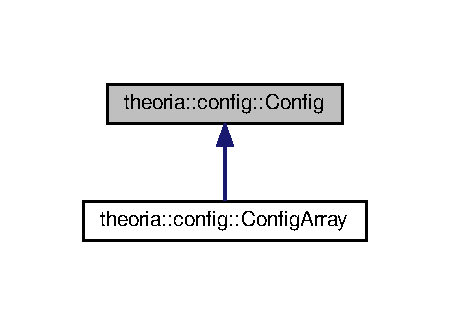
\includegraphics[width=216pt]{classtheoria_1_1config_1_1Config__inherit__graph}
\end{center}
\end{figure}


Collaboration diagram for theoria\+:\+:config\+:\+:Config\+:
\nopagebreak
\begin{figure}[H]
\begin{center}
\leavevmode
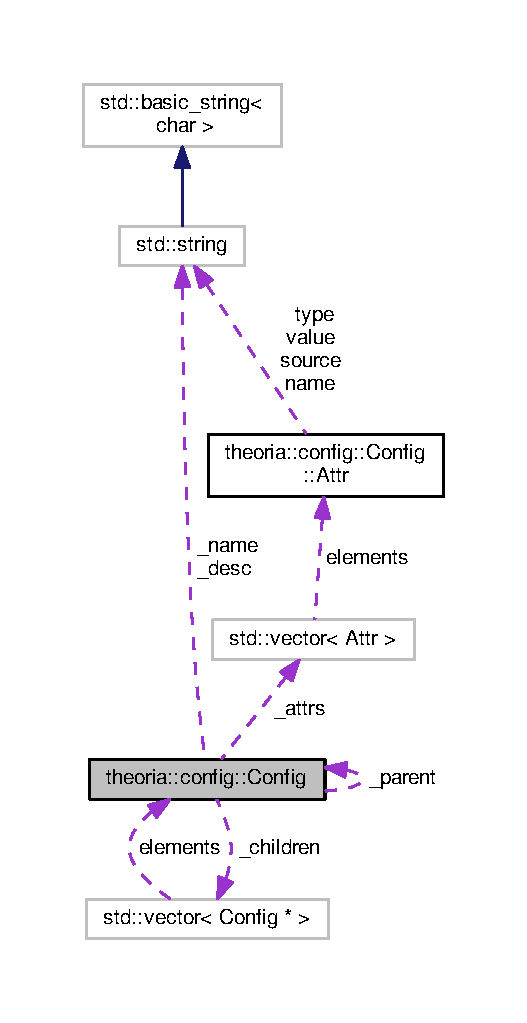
\includegraphics[width=253pt]{classtheoria_1_1config_1_1Config__coll__graph}
\end{center}
\end{figure}
\subsection*{Classes}
\begin{DoxyCompactItemize}
\item 
struct \hyperlink{structtheoria_1_1config_1_1Config_1_1Attr}{Attr}
\end{DoxyCompactItemize}
\subsection*{Public Types}
\begin{DoxyCompactItemize}
\item 
\hypertarget{classtheoria_1_1config_1_1Config_a61230728ffa4d92667a536c8c0f0ca30}{using {\bfseries Const\+Config\+List} = std\+::vector$<$ const \hyperlink{classtheoria_1_1config_1_1Config}{Config} $\ast$ $>$}\label{classtheoria_1_1config_1_1Config_a61230728ffa4d92667a536c8c0f0ca30}

\item 
\hypertarget{classtheoria_1_1config_1_1Config_a293ebfd7146d935e232a066f7e6fa279}{using {\bfseries Config\+Predicate} = std\+::function$<$ bool(const \hyperlink{classtheoria_1_1config_1_1Config}{Config} $\ast$)$>$}\label{classtheoria_1_1config_1_1Config_a293ebfd7146d935e232a066f7e6fa279}

\end{DoxyCompactItemize}
\subsection*{Public Member Functions}
\begin{DoxyCompactItemize}
\item 
\hypertarget{classtheoria_1_1config_1_1Config_a7576e899a6608ee9362e079959dac24c}{Attrs\+::const\+\_\+iterator {\bfseries find\+Attr} (const std\+::string \&name) const }\label{classtheoria_1_1config_1_1Config_a7576e899a6608ee9362e079959dac24c}

\item 
\hypertarget{classtheoria_1_1config_1_1Config_ac30090b5eedf4126046d7ace48b5fa40}{const \hyperlink{classtheoria_1_1config_1_1Config}{Config} $\ast$ {\bfseries get\+Parent} () const noexcept}\label{classtheoria_1_1config_1_1Config_ac30090b5eedf4126046d7ace48b5fa40}

\item 
\hypertarget{classtheoria_1_1config_1_1Config_a612dc92ad47937e7d1291d040252b860}{bool {\bfseries has\+Child} (const \hyperlink{classtheoria_1_1config_1_1Config}{Config} $\ast$child) const }\label{classtheoria_1_1config_1_1Config_a612dc92ad47937e7d1291d040252b860}

\item 
\hypertarget{classtheoria_1_1config_1_1Config_a5f37f0b2a36a64af46d3371ccbc0dd53}{int {\bfseries num\+Children} () const }\label{classtheoria_1_1config_1_1Config_a5f37f0b2a36a64af46d3371ccbc0dd53}

\item 
\hypertarget{classtheoria_1_1config_1_1Config_a2bfdab537ca5358f85d0e4ae8014b949}{Const\+Config\+List {\bfseries get\+Children} () const }\label{classtheoria_1_1config_1_1Config_a2bfdab537ca5358f85d0e4ae8014b949}

\item 
\hypertarget{classtheoria_1_1config_1_1Config_a8dffcbfc38e95e42d0357ebb112d7b62}{Const\+Config\+List {\bfseries get\+Children} (const Config\+Predicate \&predicate) const }\label{classtheoria_1_1config_1_1Config_a8dffcbfc38e95e42d0357ebb112d7b62}

\item 
\hypertarget{classtheoria_1_1config_1_1Config_a88395f87ae17b549a2e67297962a7a83}{const \hyperlink{classtheoria_1_1config_1_1Config}{Config} $\ast$ {\bfseries get\+Child} (const std\+::string \&name) const }\label{classtheoria_1_1config_1_1Config_a88395f87ae17b549a2e67297962a7a83}

\item 
\hypertarget{classtheoria_1_1config_1_1Config_afde7d3bd799b8f275bf8c30ffa9a28c9}{Const\+Config\+List {\bfseries get\+Siblings} () const }\label{classtheoria_1_1config_1_1Config_afde7d3bd799b8f275bf8c30ffa9a28c9}

\item 
\hypertarget{classtheoria_1_1config_1_1Config_af0c8d99efb84a611e0ec7cb95350796e}{Const\+Config\+List {\bfseries get\+Siblings} (const Config\+Predicate \&predicate) const }\label{classtheoria_1_1config_1_1Config_af0c8d99efb84a611e0ec7cb95350796e}

\item 
\hypertarget{classtheoria_1_1config_1_1Config_ad50b474daddfbec84d7e610f7687fb04}{bool {\bfseries is\+Root} () const noexcept}\label{classtheoria_1_1config_1_1Config_ad50b474daddfbec84d7e610f7687fb04}

\item 
\hypertarget{classtheoria_1_1config_1_1Config_ad5c77fb1f86a7df2dce21972f921da33}{bool {\bfseries is\+Leaf} () const noexcept}\label{classtheoria_1_1config_1_1Config_ad5c77fb1f86a7df2dce21972f921da33}

\item 
\hypertarget{classtheoria_1_1config_1_1Config_af4929f1c9b86576fdc439051a10f89cd}{const std\+::string \& {\bfseries name} () const noexcept}\label{classtheoria_1_1config_1_1Config_af4929f1c9b86576fdc439051a10f89cd}

\item 
\hypertarget{classtheoria_1_1config_1_1Config_a4d6b2e26d1139819769eaf6bb959b034}{std\+::string {\bfseries desc} () const noexcept}\label{classtheoria_1_1config_1_1Config_a4d6b2e26d1139819769eaf6bb959b034}

\item 
\hypertarget{classtheoria_1_1config_1_1Config_a5c507593cfe95c57f3f37a45d07ecedd}{bool {\bfseries has\+Attr} (const std\+::string \&name) const }\label{classtheoria_1_1config_1_1Config_a5c507593cfe95c57f3f37a45d07ecedd}

\item 
\hypertarget{classtheoria_1_1config_1_1Config_ab87a7192f2b8abeaaf452e31a6ce767d}{int {\bfseries num\+Attr} () const }\label{classtheoria_1_1config_1_1Config_ab87a7192f2b8abeaaf452e31a6ce767d}

\item 
\hypertarget{classtheoria_1_1config_1_1Config_a120102b4654bbe5ff2722ed6e1292737}{{\footnotesize template$<$class T $>$ }\\T {\bfseries get\+Attr} (const std\+::string \&name) const }\label{classtheoria_1_1config_1_1Config_a120102b4654bbe5ff2722ed6e1292737}

\item 
\hypertarget{classtheoria_1_1config_1_1Config_ad05bba9dcd7dc78b999f2825fd99f8e0}{{\footnotesize template$<$class T $>$ }\\T {\bfseries get\+Attr} (const std\+::string \&name, const T \&def) const noexcept}\label{classtheoria_1_1config_1_1Config_ad05bba9dcd7dc78b999f2825fd99f8e0}

\item 
\hypertarget{classtheoria_1_1config_1_1Config_a45702e009219115ee14b11ad1f0a851a}{std\+::string {\bfseries get\+Attr\+As\+Str} (const std\+::string \&name, const std\+::string \&def=\char`\"{}\char`\"{}) const noexcept}\label{classtheoria_1_1config_1_1Config_a45702e009219115ee14b11ad1f0a851a}

\item 
\hypertarget{classtheoria_1_1config_1_1Config_acd4660c288694e027f9ed14a89895b5e}{int {\bfseries get\+Attr\+As\+Int} (const std\+::string \&name, int def=0) const }\label{classtheoria_1_1config_1_1Config_acd4660c288694e027f9ed14a89895b5e}

\item 
\hypertarget{classtheoria_1_1config_1_1Config_a7607c7ba217b44f91417acaf98936478}{double {\bfseries get\+Attr\+As\+Dbl} (const std\+::string \&name, double def=0.\+0) const }\label{classtheoria_1_1config_1_1Config_a7607c7ba217b44f91417acaf98936478}

\item 
\hypertarget{classtheoria_1_1config_1_1Config_a9015778d5985ada7d8045e5dfa8e69f6}{bool {\bfseries get\+Attr\+As\+Bool} (const std\+::string \&name, bool def=false) const }\label{classtheoria_1_1config_1_1Config_a9015778d5985ada7d8045e5dfa8e69f6}

\item 
\hypertarget{classtheoria_1_1config_1_1Config_a2d8c81f013dd5e87e43f1f4a21162201}{virtual bool {\bfseries is\+Array} () const }\label{classtheoria_1_1config_1_1Config_a2d8c81f013dd5e87e43f1f4a21162201}

\item 
\hypertarget{classtheoria_1_1config_1_1Config_aa8d858b3ab9b56a8c566b7e890843e08}{virtual void {\bfseries to\+T\+O\+M\+L} (std\+::ostream \&out) const }\label{classtheoria_1_1config_1_1Config_aa8d858b3ab9b56a8c566b7e890843e08}

\item 
\hypertarget{classtheoria_1_1config_1_1Config_a26d27af57132772eae7ff0c3b2311556}{Attrs\+::const\+\_\+iterator {\bfseries begin\+Attr} () const }\label{classtheoria_1_1config_1_1Config_a26d27af57132772eae7ff0c3b2311556}

\item 
\hypertarget{classtheoria_1_1config_1_1Config_a9f037f8ab8d97a71f066c2f359574d68}{Attrs\+::const\+\_\+iterator {\bfseries end\+Attr} () const }\label{classtheoria_1_1config_1_1Config_a9f037f8ab8d97a71f066c2f359574d68}

\end{DoxyCompactItemize}
\subsection*{Protected Types}
\begin{DoxyCompactItemize}
\item 
\hypertarget{classtheoria_1_1config_1_1Config_ac1325f2d355e7c617dcd16d561ee2429}{using {\bfseries Text} = std\+::string}\label{classtheoria_1_1config_1_1Config_ac1325f2d355e7c617dcd16d561ee2429}

\item 
\hypertarget{classtheoria_1_1config_1_1Config_a3590578a57d530fe1e51d25b0e492f7d}{using {\bfseries Attrs} = std\+::vector$<$ \hyperlink{structtheoria_1_1config_1_1Config_1_1Attr}{Attr} $>$}\label{classtheoria_1_1config_1_1Config_a3590578a57d530fe1e51d25b0e492f7d}

\item 
\hypertarget{classtheoria_1_1config_1_1Config_acc6cccfd7dd23be9bbd053c55a1e8eb7}{using {\bfseries Children} = std\+::vector$<$ \hyperlink{classtheoria_1_1config_1_1Config}{Config} $\ast$ $>$}\label{classtheoria_1_1config_1_1Config_acc6cccfd7dd23be9bbd053c55a1e8eb7}

\end{DoxyCompactItemize}
\subsection*{Protected Member Functions}
\begin{DoxyCompactItemize}
\item 
\hypertarget{classtheoria_1_1config_1_1Config_a232146edc23baa804dbc82ffd3158f49}{{\bfseries Config} (const std\+::string \&name, const std\+::string \&desc)}\label{classtheoria_1_1config_1_1Config_a232146edc23baa804dbc82ffd3158f49}

\item 
\hypertarget{classtheoria_1_1config_1_1Config_a043dff1e32568ef63eb10c557e6f672d}{void {\bfseries add\+Attr} (const std\+::string \&name, const std\+::string \&value, const std\+::string \&type=\char`\"{}\char`\"{})}\label{classtheoria_1_1config_1_1Config_a043dff1e32568ef63eb10c557e6f672d}

\item 
\hypertarget{classtheoria_1_1config_1_1Config_ad96085447d36129bb53057c28bc43e4b}{void {\bfseries add\+Child} (\hyperlink{classtheoria_1_1config_1_1Config}{Config} $\ast$child, bool allow\+Dups=false)}\label{classtheoria_1_1config_1_1Config_ad96085447d36129bb53057c28bc43e4b}

\item 
\hypertarget{classtheoria_1_1config_1_1Config_a5c3e05b3d7119443b0bcb61eb0404829}{Attrs\+::iterator {\bfseries find\+Attr} (const std\+::string \&name)}\label{classtheoria_1_1config_1_1Config_a5c3e05b3d7119443b0bcb61eb0404829}

\item 
\hypertarget{classtheoria_1_1config_1_1Config_adc788e451cd49c6b2c85948bf8f9fb21}{Attrs\+::iterator {\bfseries end\+Attr} ()}\label{classtheoria_1_1config_1_1Config_adc788e451cd49c6b2c85948bf8f9fb21}

\item 
\hypertarget{classtheoria_1_1config_1_1Config_a75b3cca96301a65a4eef01d5c36166c6}{void {\bfseries set\+Name} (const std\+::string \&name)}\label{classtheoria_1_1config_1_1Config_a75b3cca96301a65a4eef01d5c36166c6}

\item 
\hypertarget{classtheoria_1_1config_1_1Config_adf4e6820b56f6ae52678b493819504ac}{void {\bfseries set\+Desc} (const std\+::string \&desc)}\label{classtheoria_1_1config_1_1Config_adf4e6820b56f6ae52678b493819504ac}

\end{DoxyCompactItemize}
\subsection*{Protected Attributes}
\begin{DoxyCompactItemize}
\item 
\hypertarget{classtheoria_1_1config_1_1Config_a3a4838b605d99ce710ec0ad4c5285e5d}{std\+::string {\bfseries \+\_\+name}}\label{classtheoria_1_1config_1_1Config_a3a4838b605d99ce710ec0ad4c5285e5d}

\item 
\hypertarget{classtheoria_1_1config_1_1Config_ab73d2f2163ddb788e877900ed075273e}{Text {\bfseries \+\_\+desc}}\label{classtheoria_1_1config_1_1Config_ab73d2f2163ddb788e877900ed075273e}

\item 
\hypertarget{classtheoria_1_1config_1_1Config_aecbf5fc3dcb43d90e8ebffd0650c3831}{\hyperlink{classtheoria_1_1config_1_1Config}{Config} $\ast$ {\bfseries \+\_\+parent}}\label{classtheoria_1_1config_1_1Config_aecbf5fc3dcb43d90e8ebffd0650c3831}

\item 
\hypertarget{classtheoria_1_1config_1_1Config_a51f52887f1e69984334896dc61b5846f}{Children {\bfseries \+\_\+children}}\label{classtheoria_1_1config_1_1Config_a51f52887f1e69984334896dc61b5846f}

\item 
\hypertarget{classtheoria_1_1config_1_1Config_a9ffb513d50db0712eb085f22c2c102b2}{Attrs {\bfseries \+\_\+attrs}}\label{classtheoria_1_1config_1_1Config_a9ffb513d50db0712eb085f22c2c102b2}

\end{DoxyCompactItemize}
\subsection*{Friends}
\begin{DoxyCompactItemize}
\item 
\hypertarget{classtheoria_1_1config_1_1Config_a3d61732fded713b38fc7f9fe3d80e2ae}{class {\bfseries Config\+Builder}}\label{classtheoria_1_1config_1_1Config_a3d61732fded713b38fc7f9fe3d80e2ae}

\end{DoxyCompactItemize}


The documentation for this class was generated from the following files\+:\begin{DoxyCompactItemize}
\item 
include/theoria/config/Config.\+h\item 
src/config/Config.\+cpp\end{DoxyCompactItemize}

\hypertarget{classtheoria_1_1config_1_1ConfigArray}{}\section{theoria\+:\+:config\+:\+:Config\+Array Class Reference}
\label{classtheoria_1_1config_1_1ConfigArray}\index{theoria\+::config\+::\+Config\+Array@{theoria\+::config\+::\+Config\+Array}}


Inheritance diagram for theoria\+:\+:config\+:\+:Config\+Array\+:
\nopagebreak
\begin{figure}[H]
\begin{center}
\leavevmode
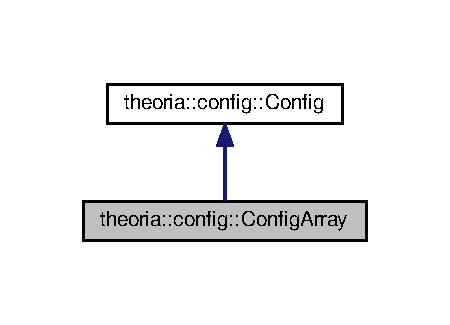
\includegraphics[width=216pt]{classtheoria_1_1config_1_1ConfigArray__inherit__graph}
\end{center}
\end{figure}


Collaboration diagram for theoria\+:\+:config\+:\+:Config\+Array\+:
\nopagebreak
\begin{figure}[H]
\begin{center}
\leavevmode
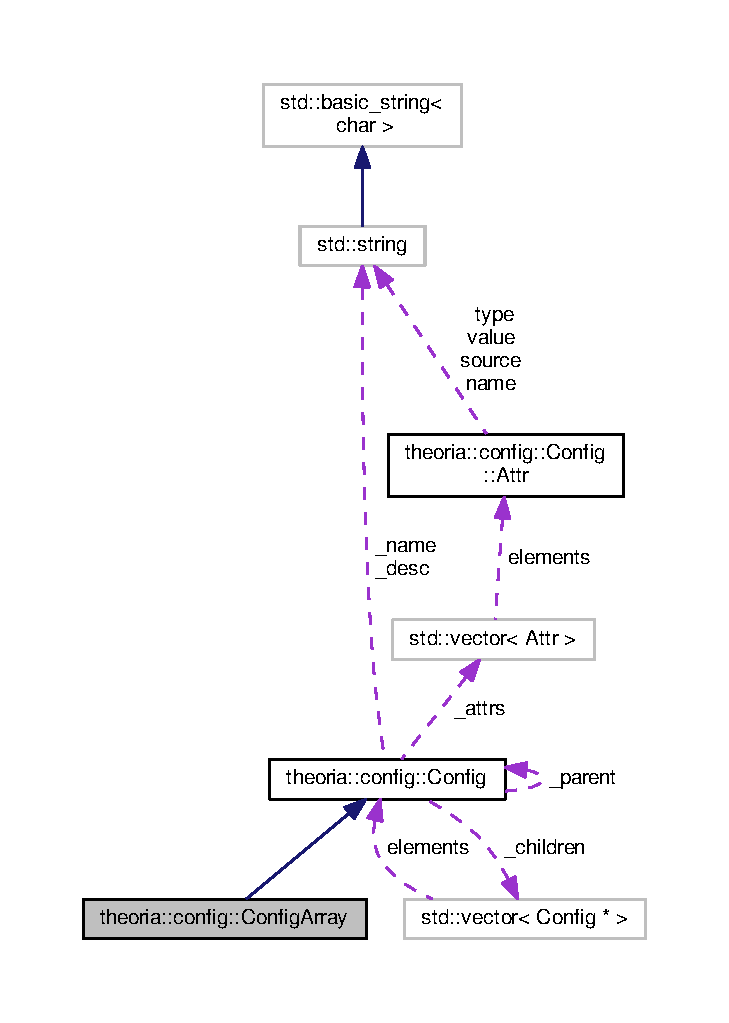
\includegraphics[width=350pt]{classtheoria_1_1config_1_1ConfigArray__coll__graph}
\end{center}
\end{figure}
\subsection*{Public Types}
\begin{DoxyCompactItemize}
\item 
\mbox{\Hypertarget{classtheoria_1_1config_1_1ConfigArray_ace80948768681e7eb033825f4fe761f2}\label{classtheoria_1_1config_1_1ConfigArray_ace80948768681e7eb033825f4fe761f2}} 
using {\bfseries const\+\_\+iterator} = Children\+::const\+\_\+iterator
\end{DoxyCompactItemize}
\subsection*{Public Member Functions}
\begin{DoxyCompactItemize}
\item 
\mbox{\Hypertarget{classtheoria_1_1config_1_1ConfigArray_a1c73dba526ebd747682bc961676f5158}\label{classtheoria_1_1config_1_1ConfigArray_a1c73dba526ebd747682bc961676f5158}} 
virtual void {\bfseries to\+T\+O\+ML} (std\+::ostream \&out) const
\item 
\mbox{\Hypertarget{classtheoria_1_1config_1_1ConfigArray_aa225cf405229bccfcfdf2042e44da4f7}\label{classtheoria_1_1config_1_1ConfigArray_aa225cf405229bccfcfdf2042e44da4f7}} 
virtual bool {\bfseries is\+Array} () const
\item 
\mbox{\Hypertarget{classtheoria_1_1config_1_1ConfigArray_a21700ff304de1c383f7e40dc6bd72cdf}\label{classtheoria_1_1config_1_1ConfigArray_a21700ff304de1c383f7e40dc6bd72cdf}} 
bool {\bfseries has\+Element} (const \hyperlink{classtheoria_1_1config_1_1Config}{Config} $\ast$child) const
\item 
\mbox{\Hypertarget{classtheoria_1_1config_1_1ConfigArray_a8482627e5891b1c15f177f5118ec484d}\label{classtheoria_1_1config_1_1ConfigArray_a8482627e5891b1c15f177f5118ec484d}} 
int {\bfseries num\+Elements} () const
\item 
\mbox{\Hypertarget{classtheoria_1_1config_1_1ConfigArray_a91bf929f72cc8eeb399df049c5008898}\label{classtheoria_1_1config_1_1ConfigArray_a91bf929f72cc8eeb399df049c5008898}} 
Const\+Config\+List {\bfseries get\+Elements} () const
\item 
\mbox{\Hypertarget{classtheoria_1_1config_1_1ConfigArray_a45cf4c898888e5ec602d4f21ab603687}\label{classtheoria_1_1config_1_1ConfigArray_a45cf4c898888e5ec602d4f21ab603687}} 
Const\+Config\+List {\bfseries get\+Elements} (const Config\+Predicate \&predicate) const
\item 
\mbox{\Hypertarget{classtheoria_1_1config_1_1ConfigArray_a7200bc93265f3b9d9b5ea462fca4a0cb}\label{classtheoria_1_1config_1_1ConfigArray_a7200bc93265f3b9d9b5ea462fca4a0cb}} 
const \hyperlink{classtheoria_1_1config_1_1Config}{Config} $\ast$ {\bfseries at} (int index) const
\item 
\mbox{\Hypertarget{classtheoria_1_1config_1_1ConfigArray_a752c88b79f88e9cd5f6a887b1b6ed119}\label{classtheoria_1_1config_1_1ConfigArray_a752c88b79f88e9cd5f6a887b1b6ed119}} 
const \hyperlink{classtheoria_1_1config_1_1Config}{Config} $\ast$ {\bfseries operator\mbox{[}$\,$\mbox{]}} (int index) const
\item 
\mbox{\Hypertarget{classtheoria_1_1config_1_1ConfigArray_a21faee00f3613c6c36a044c7a37de609}\label{classtheoria_1_1config_1_1ConfigArray_a21faee00f3613c6c36a044c7a37de609}} 
const\+\_\+iterator {\bfseries begin} () const
\item 
\mbox{\Hypertarget{classtheoria_1_1config_1_1ConfigArray_a5fca8609f50e2cfc41d75b0d6891c415}\label{classtheoria_1_1config_1_1ConfigArray_a5fca8609f50e2cfc41d75b0d6891c415}} 
const\+\_\+iterator {\bfseries end} () const
\end{DoxyCompactItemize}
\subsection*{Protected Member Functions}
\begin{DoxyCompactItemize}
\item 
\mbox{\Hypertarget{classtheoria_1_1config_1_1ConfigArray_a9086dda6fa6d659256f50be797dfe719}\label{classtheoria_1_1config_1_1ConfigArray_a9086dda6fa6d659256f50be797dfe719}} 
{\bfseries Config\+Array} (const std\+::string \&name)
\end{DoxyCompactItemize}
\subsection*{Friends}
\begin{DoxyCompactItemize}
\item 
\mbox{\Hypertarget{classtheoria_1_1config_1_1ConfigArray_a3d61732fded713b38fc7f9fe3d80e2ae}\label{classtheoria_1_1config_1_1ConfigArray_a3d61732fded713b38fc7f9fe3d80e2ae}} 
class {\bfseries Config\+Builder}
\end{DoxyCompactItemize}
\subsection*{Additional Inherited Members}


The documentation for this class was generated from the following files\+:\begin{DoxyCompactItemize}
\item 
include/theoria/config/Config.\+h\item 
src/config/Config.\+cpp\end{DoxyCompactItemize}

\hypertarget{classtheoria_1_1config_1_1ConfigBuilder}{}\section{theoria\+:\+:config\+:\+:Config\+Builder Class Reference}
\label{classtheoria_1_1config_1_1ConfigBuilder}\index{theoria\+::config\+::\+Config\+Builder@{theoria\+::config\+::\+Config\+Builder}}


{\ttfamily \#include $<$Builder.\+h$>$}



Inheritance diagram for theoria\+:\+:config\+:\+:Config\+Builder\+:\nopagebreak
\begin{figure}[H]
\begin{center}
\leavevmode
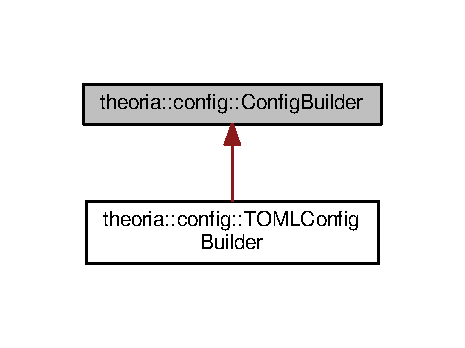
\includegraphics[width=223pt]{classtheoria_1_1config_1_1ConfigBuilder__inherit__graph}
\end{center}
\end{figure}
\subsection*{Public Types}
\begin{DoxyCompactItemize}
\item 
using \hyperlink{classtheoria_1_1config_1_1ConfigBuilder_a31d4cfc983e8ad468c483822731d790f}{Config\+Ptr} = std\+::unique\+\_\+ptr$<$ \hyperlink{classtheoria_1_1config_1_1Config}{Config} $>$
\end{DoxyCompactItemize}
\subsection*{Public Member Functions}
\begin{DoxyCompactItemize}
\item 
\hyperlink{classtheoria_1_1config_1_1ConfigBuilder_a8344379e6c6faa7bab5292abf60bb7ca}{Config\+Builder} ()
\item 
\hyperlink{classtheoria_1_1config_1_1ConfigBuilder_adf10af8634fe6ce1af5627e2c1ae8baa}{Config\+Builder} (\hyperlink{classtheoria_1_1config_1_1ConfigVariableResolver}{Config\+Variable\+Resolver} $\ast$p\+Resolver)
\item 
void \hyperlink{classtheoria_1_1config_1_1ConfigBuilder_aff25e4ada86baf419820b610a4707cbe}{set\+Resolver} (\hyperlink{classtheoria_1_1config_1_1ConfigVariableResolver}{Config\+Variable\+Resolver} $\ast$p\+Resolver)
\item 
void \hyperlink{classtheoria_1_1config_1_1ConfigBuilder_ad7542393581c33259aae6d07d11391dd}{push\+Config} (const std\+::string \&name, const std\+::string \&desc=\char`\"{}\char`\"{})
\item 
void \hyperlink{classtheoria_1_1config_1_1ConfigBuilder_a2dc70e43627e67521bf921152ee3c131}{push\+Config} (\hyperlink{classtheoria_1_1config_1_1Config}{Config} $\ast$config)
\item 
void \hyperlink{classtheoria_1_1config_1_1ConfigBuilder_a38baf2a30a0be4a5e99969c07223bc9b}{push\+Config\+Array} (const std\+::string \&name)
\item 
void \hyperlink{classtheoria_1_1config_1_1ConfigBuilder_ac58bdaa4a914c8ad0c4901128e2e7b6b}{add\+Attr} (const std\+::string \&name, const std\+::string value, const std\+::string type=\char`\"{}\char`\"{})
\item 
void \hyperlink{classtheoria_1_1config_1_1ConfigBuilder_a267121aec4f3c65ff88eb36d691ce509}{set\+Attr\+Name} (const std\+::string \&name, const std\+::string \&new\+Name)
\item 
void \hyperlink{classtheoria_1_1config_1_1ConfigBuilder_adcdd668ab4958497e7328b02ad8f8f83}{set\+Attr\+Value} (const std\+::string \&name, const std\+::string \&new\+Value)
\item 
void \hyperlink{classtheoria_1_1config_1_1ConfigBuilder_a019902280637cd43d9a69acb678a5967}{set\+Attr\+Type} (const std\+::string \&name, const std\+::string \&new\+Type)
\item 
void \hyperlink{classtheoria_1_1config_1_1ConfigBuilder_af30b50a47285d06afae1b74edfb4d762}{set\+Attr\+Source} (const std\+::string \&name, const std\+::string \&variable\+Name, const std\+::string \&resolver\+Name)
\item 
void \hyperlink{classtheoria_1_1config_1_1ConfigBuilder_acd995045c0bf17d35da9573cf53ec791}{pop\+As\+Child} (bool allow\+Dups=false)
\item 
void \hyperlink{classtheoria_1_1config_1_1ConfigBuilder_accda8a312be22d56b33adb47d5b266e9}{pop} ()
\item 
void \hyperlink{classtheoria_1_1config_1_1ConfigBuilder_a19eea792ee2bc01c44806d2a5a9f666c}{set\+Name} (const std\+::string \&name)
\item 
void \hyperlink{classtheoria_1_1config_1_1ConfigBuilder_a7aa67220439e90e9fa59082355c8186f}{set\+Desc} (const std\+::string \&desc)
\item 
\hyperlink{classtheoria_1_1config_1_1ConfigBuilder_a31d4cfc983e8ad468c483822731d790f}{Config\+Ptr} \& \hyperlink{classtheoria_1_1config_1_1ConfigBuilder_a394d42770a90532be340a8af46868f79}{top} ()
\item 
\hyperlink{classtheoria_1_1config_1_1Config}{Config} $\ast$ \hyperlink{classtheoria_1_1config_1_1ConfigBuilder_a06911a804a22e89101dab7ca3a08b049}{release\+All} ()
\item 
const \hyperlink{classtheoria_1_1config_1_1ConfigVariableResolver}{Config\+Variable\+Resolver} $\ast$ \hyperlink{classtheoria_1_1config_1_1ConfigBuilder_aa40d918441c9cbc0b60bdcd39551164f}{resolver} () const
\end{DoxyCompactItemize}


\subsection{Detailed Description}
Provides support for building config files from hierachical data files like T\+O\+ML, X\+ML, Y\+A\+ML, etc. 

\subsection{Member Typedef Documentation}
\mbox{\Hypertarget{classtheoria_1_1config_1_1ConfigBuilder_a31d4cfc983e8ad468c483822731d790f}\label{classtheoria_1_1config_1_1ConfigBuilder_a31d4cfc983e8ad468c483822731d790f}} 
\index{theoria\+::config\+::\+Config\+Builder@{theoria\+::config\+::\+Config\+Builder}!Config\+Ptr@{Config\+Ptr}}
\index{Config\+Ptr@{Config\+Ptr}!theoria\+::config\+::\+Config\+Builder@{theoria\+::config\+::\+Config\+Builder}}
\subsubsection{\texorpdfstring{Config\+Ptr}{ConfigPtr}}
{\footnotesize\ttfamily using \hyperlink{classtheoria_1_1config_1_1ConfigBuilder_a31d4cfc983e8ad468c483822731d790f}{theoria\+::config\+::\+Config\+Builder\+::\+Config\+Ptr} =  std\+::unique\+\_\+ptr$<$\hyperlink{classtheoria_1_1config_1_1Config}{Config}$>$}

Type of pointer to \hyperlink{classtheoria_1_1config_1_1Config}{Config} 

\subsection{Constructor \& Destructor Documentation}
\mbox{\Hypertarget{classtheoria_1_1config_1_1ConfigBuilder_a8344379e6c6faa7bab5292abf60bb7ca}\label{classtheoria_1_1config_1_1ConfigBuilder_a8344379e6c6faa7bab5292abf60bb7ca}} 
\index{theoria\+::config\+::\+Config\+Builder@{theoria\+::config\+::\+Config\+Builder}!Config\+Builder@{Config\+Builder}}
\index{Config\+Builder@{Config\+Builder}!theoria\+::config\+::\+Config\+Builder@{theoria\+::config\+::\+Config\+Builder}}
\subsubsection{\texorpdfstring{Config\+Builder()}{ConfigBuilder()}\hspace{0.1cm}{\footnotesize\ttfamily [1/2]}}
{\footnotesize\ttfamily theoria\+::config\+::\+Config\+Builder\+::\+Config\+Builder (\begin{DoxyParamCaption}{ }\end{DoxyParamCaption})\hspace{0.3cm}{\ttfamily [inline]}}

Construct a builder with no initial resolver \mbox{\Hypertarget{classtheoria_1_1config_1_1ConfigBuilder_adf10af8634fe6ce1af5627e2c1ae8baa}\label{classtheoria_1_1config_1_1ConfigBuilder_adf10af8634fe6ce1af5627e2c1ae8baa}} 
\index{theoria\+::config\+::\+Config\+Builder@{theoria\+::config\+::\+Config\+Builder}!Config\+Builder@{Config\+Builder}}
\index{Config\+Builder@{Config\+Builder}!theoria\+::config\+::\+Config\+Builder@{theoria\+::config\+::\+Config\+Builder}}
\subsubsection{\texorpdfstring{Config\+Builder()}{ConfigBuilder()}\hspace{0.1cm}{\footnotesize\ttfamily [2/2]}}
{\footnotesize\ttfamily theoria\+::config\+::\+Config\+Builder\+::\+Config\+Builder (\begin{DoxyParamCaption}\item[{\hyperlink{classtheoria_1_1config_1_1ConfigVariableResolver}{Config\+Variable\+Resolver} $\ast$}]{p\+Resolver }\end{DoxyParamCaption})\hspace{0.3cm}{\ttfamily [inline]}}

Construct a builder with resolver as head 
\begin{DoxyParams}{Parameters}
{\em p\+Resolver} & pointer to resolver \\
\hline
\end{DoxyParams}


\subsection{Member Function Documentation}
\mbox{\Hypertarget{classtheoria_1_1config_1_1ConfigBuilder_ac58bdaa4a914c8ad0c4901128e2e7b6b}\label{classtheoria_1_1config_1_1ConfigBuilder_ac58bdaa4a914c8ad0c4901128e2e7b6b}} 
\index{theoria\+::config\+::\+Config\+Builder@{theoria\+::config\+::\+Config\+Builder}!add\+Attr@{add\+Attr}}
\index{add\+Attr@{add\+Attr}!theoria\+::config\+::\+Config\+Builder@{theoria\+::config\+::\+Config\+Builder}}
\subsubsection{\texorpdfstring{add\+Attr()}{addAttr()}}
{\footnotesize\ttfamily void Config\+Builder\+::add\+Attr (\begin{DoxyParamCaption}\item[{const std\+::string \&}]{name,  }\item[{const std\+::string}]{value,  }\item[{const std\+::string}]{type = {\ttfamily \char`\"{}\char`\"{}} }\end{DoxyParamCaption})}

Add a attribute to the config node on top of the stack 
\begin{DoxyParams}{Parameters}
{\em name} & attribute name \\
\hline
{\em value} & attribute value \\
\hline
{\em type} & optional type hint \\
\hline
\end{DoxyParams}
\mbox{\Hypertarget{classtheoria_1_1config_1_1ConfigBuilder_accda8a312be22d56b33adb47d5b266e9}\label{classtheoria_1_1config_1_1ConfigBuilder_accda8a312be22d56b33adb47d5b266e9}} 
\index{theoria\+::config\+::\+Config\+Builder@{theoria\+::config\+::\+Config\+Builder}!pop@{pop}}
\index{pop@{pop}!theoria\+::config\+::\+Config\+Builder@{theoria\+::config\+::\+Config\+Builder}}
\subsubsection{\texorpdfstring{pop()}{pop()}}
{\footnotesize\ttfamily void Config\+Builder\+::pop (\begin{DoxyParamCaption}{ }\end{DoxyParamCaption})}

Pop the top node. It will be lost if you need not save somewhere by first calling top \mbox{\Hypertarget{classtheoria_1_1config_1_1ConfigBuilder_acd995045c0bf17d35da9573cf53ec791}\label{classtheoria_1_1config_1_1ConfigBuilder_acd995045c0bf17d35da9573cf53ec791}} 
\index{theoria\+::config\+::\+Config\+Builder@{theoria\+::config\+::\+Config\+Builder}!pop\+As\+Child@{pop\+As\+Child}}
\index{pop\+As\+Child@{pop\+As\+Child}!theoria\+::config\+::\+Config\+Builder@{theoria\+::config\+::\+Config\+Builder}}
\subsubsection{\texorpdfstring{pop\+As\+Child()}{popAsChild()}}
{\footnotesize\ttfamily void Config\+Builder\+::pop\+As\+Child (\begin{DoxyParamCaption}\item[{bool}]{allow\+Dups = {\ttfamily false} }\end{DoxyParamCaption})}

Pop a node off the stack and attach it as a chile to the new top node 
\begin{DoxyParams}{Parameters}
{\em allow\+Dups} & Normally \hyperlink{classtheoria_1_1config_1_1Config}{Config} nodes must be unique by name. Set true to override. N\+O\+TE\+: if parent is an array dups will automatically to be allowed even if allow\+Dups==false \\
\hline
\end{DoxyParams}
\mbox{\Hypertarget{classtheoria_1_1config_1_1ConfigBuilder_ad7542393581c33259aae6d07d11391dd}\label{classtheoria_1_1config_1_1ConfigBuilder_ad7542393581c33259aae6d07d11391dd}} 
\index{theoria\+::config\+::\+Config\+Builder@{theoria\+::config\+::\+Config\+Builder}!push\+Config@{push\+Config}}
\index{push\+Config@{push\+Config}!theoria\+::config\+::\+Config\+Builder@{theoria\+::config\+::\+Config\+Builder}}
\subsubsection{\texorpdfstring{push\+Config()}{pushConfig()}\hspace{0.1cm}{\footnotesize\ttfamily [1/2]}}
{\footnotesize\ttfamily void Config\+Builder\+::push\+Config (\begin{DoxyParamCaption}\item[{const std\+::string \&}]{name,  }\item[{const std\+::string \&}]{desc = {\ttfamily \char`\"{}\char`\"{}} }\end{DoxyParamCaption})}

Create a config node with name and description and push on to the node stack 
\begin{DoxyParams}{Parameters}
{\em name} & the name of the node \\
\hline
{\em desc} & the node descrition \\
\hline
\end{DoxyParams}
\mbox{\Hypertarget{classtheoria_1_1config_1_1ConfigBuilder_a2dc70e43627e67521bf921152ee3c131}\label{classtheoria_1_1config_1_1ConfigBuilder_a2dc70e43627e67521bf921152ee3c131}} 
\index{theoria\+::config\+::\+Config\+Builder@{theoria\+::config\+::\+Config\+Builder}!push\+Config@{push\+Config}}
\index{push\+Config@{push\+Config}!theoria\+::config\+::\+Config\+Builder@{theoria\+::config\+::\+Config\+Builder}}
\subsubsection{\texorpdfstring{push\+Config()}{pushConfig()}\hspace{0.1cm}{\footnotesize\ttfamily [2/2]}}
{\footnotesize\ttfamily void Config\+Builder\+::push\+Config (\begin{DoxyParamCaption}\item[{\hyperlink{classtheoria_1_1config_1_1Config}{Config} $\ast$}]{config }\end{DoxyParamCaption})}

Push an existing node to augment 
\begin{DoxyParams}{Parameters}
{\em config} & a \hyperlink{classtheoria_1_1config_1_1Config}{Config} node \\
\hline
\end{DoxyParams}
\mbox{\Hypertarget{classtheoria_1_1config_1_1ConfigBuilder_a38baf2a30a0be4a5e99969c07223bc9b}\label{classtheoria_1_1config_1_1ConfigBuilder_a38baf2a30a0be4a5e99969c07223bc9b}} 
\index{theoria\+::config\+::\+Config\+Builder@{theoria\+::config\+::\+Config\+Builder}!push\+Config\+Array@{push\+Config\+Array}}
\index{push\+Config\+Array@{push\+Config\+Array}!theoria\+::config\+::\+Config\+Builder@{theoria\+::config\+::\+Config\+Builder}}
\subsubsection{\texorpdfstring{push\+Config\+Array()}{pushConfigArray()}}
{\footnotesize\ttfamily void Config\+Builder\+::push\+Config\+Array (\begin{DoxyParamCaption}\item[{const std\+::string \&}]{name }\end{DoxyParamCaption})}

Create a \hyperlink{classtheoria_1_1config_1_1ConfigArray}{Config\+Array} node with name and push on to the node stack 
\begin{DoxyParams}{Parameters}
{\em name} & the name of the array \\
\hline
\end{DoxyParams}
\mbox{\Hypertarget{classtheoria_1_1config_1_1ConfigBuilder_a06911a804a22e89101dab7ca3a08b049}\label{classtheoria_1_1config_1_1ConfigBuilder_a06911a804a22e89101dab7ca3a08b049}} 
\index{theoria\+::config\+::\+Config\+Builder@{theoria\+::config\+::\+Config\+Builder}!release\+All@{release\+All}}
\index{release\+All@{release\+All}!theoria\+::config\+::\+Config\+Builder@{theoria\+::config\+::\+Config\+Builder}}
\subsubsection{\texorpdfstring{release\+All()}{releaseAll()}}
{\footnotesize\ttfamily \hyperlink{classtheoria_1_1config_1_1Config}{Config} $\ast$ Config\+Builder\+::release\+All (\begin{DoxyParamCaption}{ }\end{DoxyParamCaption})}

Call pop\+Child repeatedly until stack is empty then release the top element from its owning unique ptr and return it. \begin{DoxyReturn}{Returns}
the root node (the node deepest in the stack when this function was called) or nullptr if stack empty 
\end{DoxyReturn}
\mbox{\Hypertarget{classtheoria_1_1config_1_1ConfigBuilder_aa40d918441c9cbc0b60bdcd39551164f}\label{classtheoria_1_1config_1_1ConfigBuilder_aa40d918441c9cbc0b60bdcd39551164f}} 
\index{theoria\+::config\+::\+Config\+Builder@{theoria\+::config\+::\+Config\+Builder}!resolver@{resolver}}
\index{resolver@{resolver}!theoria\+::config\+::\+Config\+Builder@{theoria\+::config\+::\+Config\+Builder}}
\subsubsection{\texorpdfstring{resolver()}{resolver()}}
{\footnotesize\ttfamily const \hyperlink{classtheoria_1_1config_1_1ConfigVariableResolver}{Config\+Variable\+Resolver}$\ast$ theoria\+::config\+::\+Config\+Builder\+::resolver (\begin{DoxyParamCaption}{ }\end{DoxyParamCaption}) const\hspace{0.3cm}{\ttfamily [inline]}}

Return the head resolver of this builder\textquotesingle{}s resolver chain. Normally variable resolution is taken care of automatically so this method not typically required. Useful for unit testing. \begin{DoxyReturn}{Returns}
the head resolver 
\end{DoxyReturn}
\mbox{\Hypertarget{classtheoria_1_1config_1_1ConfigBuilder_a267121aec4f3c65ff88eb36d691ce509}\label{classtheoria_1_1config_1_1ConfigBuilder_a267121aec4f3c65ff88eb36d691ce509}} 
\index{theoria\+::config\+::\+Config\+Builder@{theoria\+::config\+::\+Config\+Builder}!set\+Attr\+Name@{set\+Attr\+Name}}
\index{set\+Attr\+Name@{set\+Attr\+Name}!theoria\+::config\+::\+Config\+Builder@{theoria\+::config\+::\+Config\+Builder}}
\subsubsection{\texorpdfstring{set\+Attr\+Name()}{setAttrName()}}
{\footnotesize\ttfamily void Config\+Builder\+::set\+Attr\+Name (\begin{DoxyParamCaption}\item[{const std\+::string \&}]{name,  }\item[{const std\+::string \&}]{new\+Name }\end{DoxyParamCaption})}

Change attributes name 
\begin{DoxyParams}{Parameters}
{\em name} & current name \\
\hline
{\em new\+Name} & the new attribute name \\
\hline
\end{DoxyParams}
\mbox{\Hypertarget{classtheoria_1_1config_1_1ConfigBuilder_af30b50a47285d06afae1b74edfb4d762}\label{classtheoria_1_1config_1_1ConfigBuilder_af30b50a47285d06afae1b74edfb4d762}} 
\index{theoria\+::config\+::\+Config\+Builder@{theoria\+::config\+::\+Config\+Builder}!set\+Attr\+Source@{set\+Attr\+Source}}
\index{set\+Attr\+Source@{set\+Attr\+Source}!theoria\+::config\+::\+Config\+Builder@{theoria\+::config\+::\+Config\+Builder}}
\subsubsection{\texorpdfstring{set\+Attr\+Source()}{setAttrSource()}}
{\footnotesize\ttfamily void Config\+Builder\+::set\+Attr\+Source (\begin{DoxyParamCaption}\item[{const std\+::string \&}]{name,  }\item[{const std\+::string \&}]{variable\+Name,  }\item[{const std\+::string \&}]{resolver\+Name }\end{DoxyParamCaption})}

Change attribute\textquotesingle{}s source to variable within resolver \mbox{\Hypertarget{classtheoria_1_1config_1_1ConfigBuilder_a019902280637cd43d9a69acb678a5967}\label{classtheoria_1_1config_1_1ConfigBuilder_a019902280637cd43d9a69acb678a5967}} 
\index{theoria\+::config\+::\+Config\+Builder@{theoria\+::config\+::\+Config\+Builder}!set\+Attr\+Type@{set\+Attr\+Type}}
\index{set\+Attr\+Type@{set\+Attr\+Type}!theoria\+::config\+::\+Config\+Builder@{theoria\+::config\+::\+Config\+Builder}}
\subsubsection{\texorpdfstring{set\+Attr\+Type()}{setAttrType()}}
{\footnotesize\ttfamily void Config\+Builder\+::set\+Attr\+Type (\begin{DoxyParamCaption}\item[{const std\+::string \&}]{name,  }\item[{const std\+::string \&}]{new\+Type }\end{DoxyParamCaption})}

Change attributes type 
\begin{DoxyParams}{Parameters}
{\em name} & the name of the attribute to change \\
\hline
{\em new\+Type} & the type name to change to (string, int, bool, double) \\
\hline
\end{DoxyParams}
\mbox{\Hypertarget{classtheoria_1_1config_1_1ConfigBuilder_adcdd668ab4958497e7328b02ad8f8f83}\label{classtheoria_1_1config_1_1ConfigBuilder_adcdd668ab4958497e7328b02ad8f8f83}} 
\index{theoria\+::config\+::\+Config\+Builder@{theoria\+::config\+::\+Config\+Builder}!set\+Attr\+Value@{set\+Attr\+Value}}
\index{set\+Attr\+Value@{set\+Attr\+Value}!theoria\+::config\+::\+Config\+Builder@{theoria\+::config\+::\+Config\+Builder}}
\subsubsection{\texorpdfstring{set\+Attr\+Value()}{setAttrValue()}}
{\footnotesize\ttfamily void Config\+Builder\+::set\+Attr\+Value (\begin{DoxyParamCaption}\item[{const std\+::string \&}]{name,  }\item[{const std\+::string \&}]{new\+Value }\end{DoxyParamCaption})}

Change attributes value 
\begin{DoxyParams}{Parameters}
{\em name} & the name of the attribute to change \\
\hline
{\em new\+Value} & the value to change to \\
\hline
\end{DoxyParams}
\mbox{\Hypertarget{classtheoria_1_1config_1_1ConfigBuilder_a7aa67220439e90e9fa59082355c8186f}\label{classtheoria_1_1config_1_1ConfigBuilder_a7aa67220439e90e9fa59082355c8186f}} 
\index{theoria\+::config\+::\+Config\+Builder@{theoria\+::config\+::\+Config\+Builder}!set\+Desc@{set\+Desc}}
\index{set\+Desc@{set\+Desc}!theoria\+::config\+::\+Config\+Builder@{theoria\+::config\+::\+Config\+Builder}}
\subsubsection{\texorpdfstring{set\+Desc()}{setDesc()}}
{\footnotesize\ttfamily void Config\+Builder\+::set\+Desc (\begin{DoxyParamCaption}\item[{const std\+::string \&}]{desc }\end{DoxyParamCaption})}

Change the description of the node on the top of the stack 
\begin{DoxyParams}{Parameters}
{\em desc} & the new description for the node \\
\hline
\end{DoxyParams}
\mbox{\Hypertarget{classtheoria_1_1config_1_1ConfigBuilder_a19eea792ee2bc01c44806d2a5a9f666c}\label{classtheoria_1_1config_1_1ConfigBuilder_a19eea792ee2bc01c44806d2a5a9f666c}} 
\index{theoria\+::config\+::\+Config\+Builder@{theoria\+::config\+::\+Config\+Builder}!set\+Name@{set\+Name}}
\index{set\+Name@{set\+Name}!theoria\+::config\+::\+Config\+Builder@{theoria\+::config\+::\+Config\+Builder}}
\subsubsection{\texorpdfstring{set\+Name()}{setName()}}
{\footnotesize\ttfamily void Config\+Builder\+::set\+Name (\begin{DoxyParamCaption}\item[{const std\+::string \&}]{name }\end{DoxyParamCaption})}

Change the name of the node on the top of the stack 
\begin{DoxyParams}{Parameters}
{\em name} & the new name for node \\
\hline
\end{DoxyParams}
\mbox{\Hypertarget{classtheoria_1_1config_1_1ConfigBuilder_aff25e4ada86baf419820b610a4707cbe}\label{classtheoria_1_1config_1_1ConfigBuilder_aff25e4ada86baf419820b610a4707cbe}} 
\index{theoria\+::config\+::\+Config\+Builder@{theoria\+::config\+::\+Config\+Builder}!set\+Resolver@{set\+Resolver}}
\index{set\+Resolver@{set\+Resolver}!theoria\+::config\+::\+Config\+Builder@{theoria\+::config\+::\+Config\+Builder}}
\subsubsection{\texorpdfstring{set\+Resolver()}{setResolver()}}
{\footnotesize\ttfamily void theoria\+::config\+::\+Config\+Builder\+::set\+Resolver (\begin{DoxyParamCaption}\item[{\hyperlink{classtheoria_1_1config_1_1ConfigVariableResolver}{Config\+Variable\+Resolver} $\ast$}]{p\+Resolver }\end{DoxyParamCaption})\hspace{0.3cm}{\ttfamily [inline]}}

Set the head resolver. Overwrites previous resolver 
\begin{DoxyParams}{Parameters}
{\em p\+Resolver} & the new resolver \\
\hline
\end{DoxyParams}
\mbox{\Hypertarget{classtheoria_1_1config_1_1ConfigBuilder_a394d42770a90532be340a8af46868f79}\label{classtheoria_1_1config_1_1ConfigBuilder_a394d42770a90532be340a8af46868f79}} 
\index{theoria\+::config\+::\+Config\+Builder@{theoria\+::config\+::\+Config\+Builder}!top@{top}}
\index{top@{top}!theoria\+::config\+::\+Config\+Builder@{theoria\+::config\+::\+Config\+Builder}}
\subsubsection{\texorpdfstring{top()}{top()}}
{\footnotesize\ttfamily \hyperlink{classtheoria_1_1config_1_1ConfigBuilder_a31d4cfc983e8ad468c483822731d790f}{Config\+Ptr} \& Config\+Builder\+::top (\begin{DoxyParamCaption}{ }\end{DoxyParamCaption})}

The node on top of the stack \begin{DoxyReturn}{Returns}
top node on the config stack 
\end{DoxyReturn}

\begin{DoxyExceptions}{Exceptions}
{\em std\+::runtime\+\_\+error} & if stack is empty \\
\hline
\end{DoxyExceptions}


The documentation for this class was generated from the following files\+:\begin{DoxyCompactItemize}
\item 
include/theoria/config/Builder.\+h\item 
src/config/Builder.\+cpp\end{DoxyCompactItemize}

\hypertarget{classtheoria_1_1config_1_1ConfigParser}{}\section{theoria\+:\+:config\+:\+:Config\+Parser Class Reference}
\label{classtheoria_1_1config_1_1ConfigParser}\index{theoria\+::config\+::\+Config\+Parser@{theoria\+::config\+::\+Config\+Parser}}


{\ttfamily \#include $<$Parser.\+h$>$}



Inheritance diagram for theoria\+:\+:config\+:\+:Config\+Parser\+:\nopagebreak
\begin{figure}[H]
\begin{center}
\leavevmode
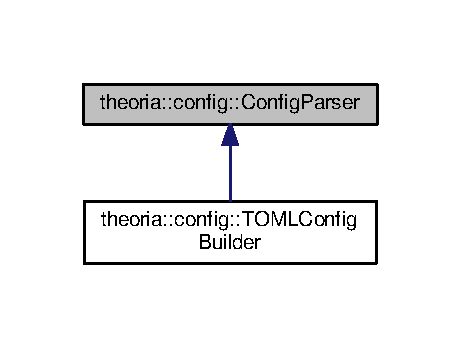
\includegraphics[width=221pt]{classtheoria_1_1config_1_1ConfigParser__inherit__graph}
\end{center}
\end{figure}
\subsection*{Public Member Functions}
\begin{DoxyCompactItemize}
\item 
virtual std\+::unique\+\_\+ptr$<$ const \hyperlink{classtheoria_1_1config_1_1Config}{Config} $>$ \hyperlink{classtheoria_1_1config_1_1ConfigParser_a4eca80a9831324237f2a2aa9a5018c89}{parse\+\_\+file} (const std\+::string \&filename)
\item 
virtual std\+::unique\+\_\+ptr$<$ const \hyperlink{classtheoria_1_1config_1_1Config}{Config} $>$ \hyperlink{classtheoria_1_1config_1_1ConfigParser_af0ccd3cc2202c3d588a977c611dfa988}{parse} (std\+::istream \&stream)=0
\end{DoxyCompactItemize}


\subsection{Detailed Description}
Interface for parsing a config file or text in a stream. Parser implementations are responsible for converting some structured textual format (e.\+g., T\+O\+ML, X\+ML, J\+S\+ON, etc.) and converting it into \hyperlink{classtheoria_1_1config_1_1Config}{Config} representation. 

\subsection{Member Function Documentation}
\mbox{\Hypertarget{classtheoria_1_1config_1_1ConfigParser_af0ccd3cc2202c3d588a977c611dfa988}\label{classtheoria_1_1config_1_1ConfigParser_af0ccd3cc2202c3d588a977c611dfa988}} 
\index{theoria\+::config\+::\+Config\+Parser@{theoria\+::config\+::\+Config\+Parser}!parse@{parse}}
\index{parse@{parse}!theoria\+::config\+::\+Config\+Parser@{theoria\+::config\+::\+Config\+Parser}}
\subsubsection{\texorpdfstring{parse()}{parse()}}
{\footnotesize\ttfamily virtual std\+::unique\+\_\+ptr$<$const \hyperlink{classtheoria_1_1config_1_1Config}{Config}$>$ theoria\+::config\+::\+Config\+Parser\+::parse (\begin{DoxyParamCaption}\item[{std\+::istream \&}]{stream }\end{DoxyParamCaption})\hspace{0.3cm}{\ttfamily [pure virtual]}}

Parse the stream and return a \hyperlink{classtheoria_1_1config_1_1Config}{Config} 
\begin{DoxyParams}{Parameters}
{\em stream} & an input stream to parse \\
\hline
\end{DoxyParams}


Implemented in \hyperlink{classtheoria_1_1config_1_1TOMLConfigBuilder_ac5a36aebe769d67decc9946ee2a3fbc3}{theoria\+::config\+::\+T\+O\+M\+L\+Config\+Builder}.

\mbox{\Hypertarget{classtheoria_1_1config_1_1ConfigParser_a4eca80a9831324237f2a2aa9a5018c89}\label{classtheoria_1_1config_1_1ConfigParser_a4eca80a9831324237f2a2aa9a5018c89}} 
\index{theoria\+::config\+::\+Config\+Parser@{theoria\+::config\+::\+Config\+Parser}!parse\+\_\+file@{parse\+\_\+file}}
\index{parse\+\_\+file@{parse\+\_\+file}!theoria\+::config\+::\+Config\+Parser@{theoria\+::config\+::\+Config\+Parser}}
\subsubsection{\texorpdfstring{parse\+\_\+file()}{parse\_file()}}
{\footnotesize\ttfamily std\+::unique\+\_\+ptr$<$ const \hyperlink{classtheoria_1_1config_1_1Config}{Config} $>$ Config\+Parser\+::parse\+\_\+file (\begin{DoxyParamCaption}\item[{const std\+::string \&}]{filename }\end{DoxyParamCaption})\hspace{0.3cm}{\ttfamily [virtual]}}

Default implementation opens the file and calls parse(with the file\textquotesingle{}s std\+::ifstream)


\begin{DoxyParams}{Parameters}
{\em filename} & the file to parse \\
\hline
\end{DoxyParams}
\begin{DoxyReturn}{Returns}
the resulting \hyperlink{classtheoria_1_1config_1_1Config}{Config} object
\end{DoxyReturn}
N\+O\+TE\+:\+: If you override parse\+\_\+file in your derived \hyperlink{classtheoria_1_1config_1_1ConfigParser}{Config\+Parser} then you can optionally implement parse or simply stub it out as Theoria will only call parse\+\_\+file directly. A stream-\/based interface is useful for writing unit tests using istringstream. 

Reimplemented in \hyperlink{classtheoria_1_1config_1_1TOMLConfigBuilder_afba5445b56e12b39cf1b266627a27f58}{theoria\+::config\+::\+T\+O\+M\+L\+Config\+Builder}.



The documentation for this class was generated from the following files\+:\begin{DoxyCompactItemize}
\item 
include/theoria/config/Parser.\+h\item 
src/config/Parser.\+cpp\end{DoxyCompactItemize}

\hypertarget{classConfigResolverBuilder}{}\section{Config\+Resolver\+Builder Class Reference}
\label{classConfigResolverBuilder}\index{Config\+Resolver\+Builder@{Config\+Resolver\+Builder}}


{\ttfamily \#include $<$Config\+Resolver\+Builder.\+h$>$}



Inheritance diagram for Config\+Resolver\+Builder\+:\nopagebreak
\begin{figure}[H]
\begin{center}
\leavevmode
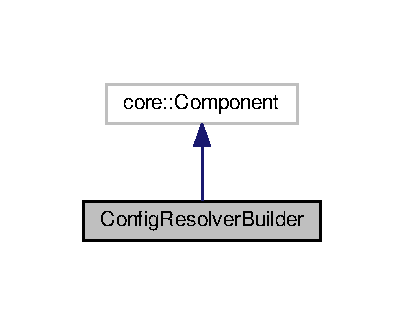
\includegraphics[width=194pt]{classConfigResolverBuilder__inherit__graph}
\end{center}
\end{figure}


Collaboration diagram for Config\+Resolver\+Builder\+:\nopagebreak
\begin{figure}[H]
\begin{center}
\leavevmode
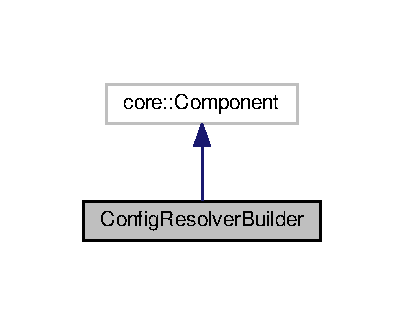
\includegraphics[width=194pt]{classConfigResolverBuilder__coll__graph}
\end{center}
\end{figure}
\subsection*{Public Member Functions}
\begin{DoxyCompactItemize}
\item 
\mbox{\Hypertarget{classConfigResolverBuilder_a4e217cbe1d663a83d098e224cc4d7cb8}\label{classConfigResolverBuilder_a4e217cbe1d663a83d098e224cc4d7cb8}} 
Dependencies {\bfseries init} (const \hyperlink{classtheoria_1_1config_1_1Config}{Config} \&config) overide
\item 
void \hyperlink{classConfigResolverBuilder_a77c367a65b4e8fb6285b63fba0bdbef0}{finalize} (Component\+List dependencies) override
\item 
\mbox{\Hypertarget{classConfigResolverBuilder_aaab8623502528a6de4129b1016f02224}\label{classConfigResolverBuilder_aaab8623502528a6de4129b1016f02224}} 
config\+::\+Config\+Variable\+Resolver $\ast$ {\bfseries build} () const
\end{DoxyCompactItemize}


\subsection{Detailed Description}
Builds a chain of resolvers. Used by Config Builder 

\subsection{Member Function Documentation}
\mbox{\Hypertarget{classConfigResolverBuilder_a77c367a65b4e8fb6285b63fba0bdbef0}\label{classConfigResolverBuilder_a77c367a65b4e8fb6285b63fba0bdbef0}} 
\index{Config\+Resolver\+Builder@{Config\+Resolver\+Builder}!finalize@{finalize}}
\index{finalize@{finalize}!Config\+Resolver\+Builder@{Config\+Resolver\+Builder}}
\subsubsection{\texorpdfstring{finalize()}{finalize()}}
{\footnotesize\ttfamily void Config\+Resolver\+Builder\+::finalize (\begin{DoxyParamCaption}\item[{Component\+List}]{dependencies }\end{DoxyParamCaption})\hspace{0.3cm}{\ttfamily [override]}}

Receives a Config\+Builder and one or more resolvers and wires the resolvers as the builders resolver chain in the order they appear 

The documentation for this class was generated from the following file\+:\begin{DoxyCompactItemize}
\item 
include/theoria/core/Config\+Resolver\+Builder.\+h\end{DoxyCompactItemize}

\hypertarget{classtheoria_1_1config_1_1ConfigVariableResolver}{}\section{theoria\+:\+:config\+:\+:Config\+Variable\+Resolver Class Reference}
\label{classtheoria_1_1config_1_1ConfigVariableResolver}\index{theoria\+::config\+::\+Config\+Variable\+Resolver@{theoria\+::config\+::\+Config\+Variable\+Resolver}}


{\ttfamily \#include $<$Resolve.\+h$>$}



Inheritance diagram for theoria\+:\+:config\+:\+:Config\+Variable\+Resolver\+:\nopagebreak
\begin{figure}[H]
\begin{center}
\leavevmode
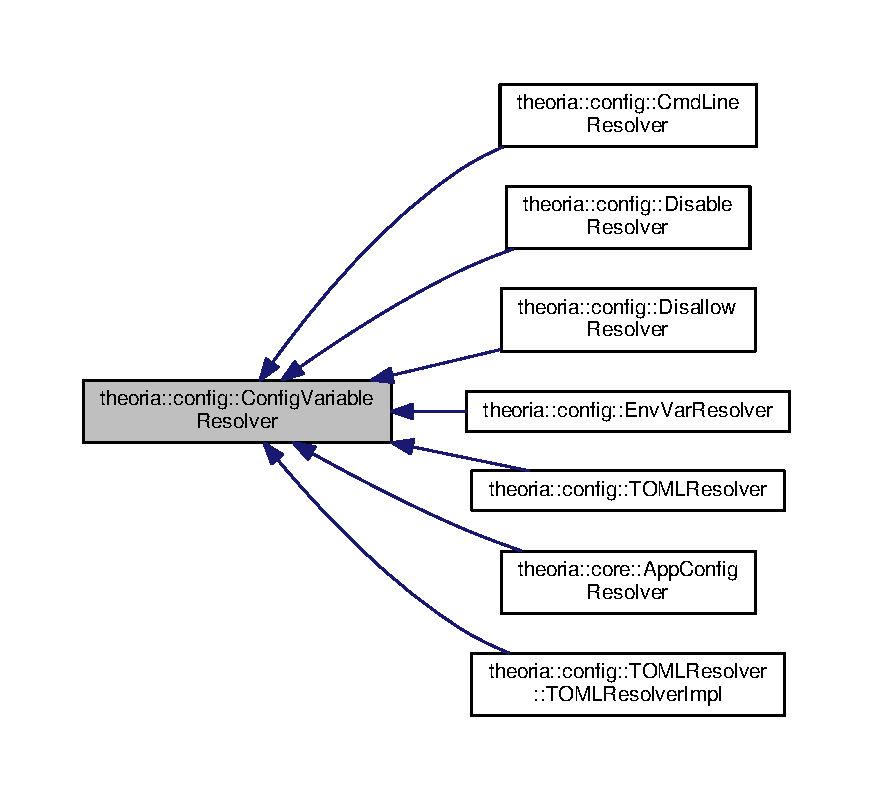
\includegraphics[width=350pt]{classtheoria_1_1config_1_1ConfigVariableResolver__inherit__graph}
\end{center}
\end{figure}
\subsection*{Public Types}
\begin{DoxyCompactItemize}
\item 
using \hyperlink{classtheoria_1_1config_1_1ConfigVariableResolver_af27a85262d802c9ad4ecb1179efaf447}{Result} = std\+::pair$<$ const \hyperlink{classtheoria_1_1config_1_1ConfigVariableResolver}{Config\+Variable\+Resolver} $\ast$, std\+::string $>$
\item 
using \hyperlink{classtheoria_1_1config_1_1ConfigVariableResolver_a2d92a11d55181183ce4071566437f01b}{Result\+Vec} = std\+::vector$<$ \hyperlink{classtheoria_1_1config_1_1ConfigVariableResolver_af27a85262d802c9ad4ecb1179efaf447}{Result} $>$
\end{DoxyCompactItemize}
\subsection*{Public Member Functions}
\begin{DoxyCompactItemize}
\item 
\hyperlink{classtheoria_1_1config_1_1ConfigVariableResolver_a90e26596be3efc1597909fd615a6a286}{Config\+Variable\+Resolver} ()
\item 
virtual \hyperlink{classtheoria_1_1config_1_1ConfigVariableResolver_ac395c02cf0dc162c093bfda494e3af0b}{$\sim$\+Config\+Variable\+Resolver} ()
\item 
std\+::string \hyperlink{classtheoria_1_1config_1_1ConfigVariableResolver_acb155f953e0d353cbd4966ae0d6e50da}{resolve} (const std\+::string \&var) const
\item 
\hyperlink{classtheoria_1_1config_1_1ConfigVariableResolver_a2d92a11d55181183ce4071566437f01b}{Result\+Vec} \hyperlink{classtheoria_1_1config_1_1ConfigVariableResolver_a406e1024b865b1749c920c83b774b745}{resolve\+All} (const std\+::string \&var) const
\end{DoxyCompactItemize}
\subsection*{is the name of the variable (with no leading \textquotesingle{}\$\textquotesingle{})}
\label{_amgrpa55251cdd20cd6c833ba352b7e8d9b84}%
Abstract method that implements local resolution for a specific type of resolver.

\begin{DoxyReturn}{Returns}
std\+::pair$<$\char`\"{}\textquotesingle{}resolver\textquotesingle{}\char`\"{}, \char`\"{}\textquotesingle{}value\textquotesingle{}\char`\"{}$>$ if found or std\+::pair$<$\char`\"{}\char`\"{},\char`\"{}\char`\"{}$>$ if not found 
\end{DoxyReturn}
\begin{DoxyCompactItemize}
\item 
\mbox{\Hypertarget{classtheoria_1_1config_1_1ConfigVariableResolver_a85e75133c0fdd67dd8b1d8e678f46ca8}\label{classtheoria_1_1config_1_1ConfigVariableResolver_a85e75133c0fdd67dd8b1d8e678f46ca8}} 
virtual \hyperlink{classtheoria_1_1config_1_1ConfigVariableResolver_af27a85262d802c9ad4ecb1179efaf447}{Result} {\bfseries lookup} (const std\+::string \&\hyperlink{classtheoria_1_1config_1_1ConfigVariableResolver_a026bda729faf988eaef334a45ec92303}{name}) const =0
\item 
virtual std\+::string \hyperlink{classtheoria_1_1config_1_1ConfigVariableResolver_a026bda729faf988eaef334a45ec92303}{name} () const =0
\item 
void \hyperlink{classtheoria_1_1config_1_1ConfigVariableResolver_aedd40aea06645632c2b380c0181c563b}{append} (\hyperlink{classtheoria_1_1config_1_1ConfigVariableResolver}{Config\+Variable\+Resolver} $\ast$resolver)
\item 
const \hyperlink{classtheoria_1_1config_1_1ConfigVariableResolver}{Config\+Variable\+Resolver} $\ast$ \hyperlink{classtheoria_1_1config_1_1ConfigVariableResolver_a2861f6405c8b8e6c8c267dd490c46d2a}{next} () const
\end{DoxyCompactItemize}


\subsection{Detailed Description}
Base configuration variable resolver.

Theoria configuration files can contain variables of the form {\itshape \$variable} (\textquotesingle{}first variables\textquotesingle{}) and {\itshape \$\$variable} (\textquotesingle{}last variables \textquotesingle{}) . Resolvers determine how a variable is bound to a value. Resolvers can be chained together in a sequence so that the value of a variable can be determined by walking a list of different resolvers.

{\itshape First Variables} (\$var) are bound by the first resolver that recognizes the variable {\itshape Last Variables} (\$\$var) are bound by the last resolver that recognizes the variable

Example Config\+Variable\+Resolvers are\+:\begin{DoxyVerb}<CmdLineResolver>, <EnvVarResolver>, <ConfigVariableResolver>, <TomlResolver> \end{DoxyVerb}


Say you want your project to be configurable from both the command line and environment and you want the command line to take precedence. This means if a variable is give a value on the command line ignore any value in the env.

For this you should use\+: \hyperlink{classtheoria_1_1config_1_1CmdLineResolver}{Cmd\+Line\+Resolver} -\/$>$ \hyperlink{classtheoria_1_1config_1_1EnvVarResolver}{Env\+Var\+Resolver} and variables of the form \$va1, \$var2 and so on. But suppose for some specific variable you don\textquotesingle{}t want the user to change it if it is defined in the env. You can still use the same resolver chain but make this a {\itshape last variable} \$\$special\+Var

A general guideline is to construct your resolver chain such that most variables are \$first and only used \$\$last syntax for special exceptions. Many projects can probably avoid \$\$last variables all together.

Theoria will output a representation of your config file at runtime that shows how variables were resolved. You can also run a project using\+: {\itshape theoria --resolve-\/only} to see the same with out executing the code 

\subsection{Member Typedef Documentation}
\mbox{\Hypertarget{classtheoria_1_1config_1_1ConfigVariableResolver_af27a85262d802c9ad4ecb1179efaf447}\label{classtheoria_1_1config_1_1ConfigVariableResolver_af27a85262d802c9ad4ecb1179efaf447}} 
\index{theoria\+::config\+::\+Config\+Variable\+Resolver@{theoria\+::config\+::\+Config\+Variable\+Resolver}!Result@{Result}}
\index{Result@{Result}!theoria\+::config\+::\+Config\+Variable\+Resolver@{theoria\+::config\+::\+Config\+Variable\+Resolver}}
\subsubsection{\texorpdfstring{Result}{Result}}
{\footnotesize\ttfamily using \hyperlink{classtheoria_1_1config_1_1ConfigVariableResolver_af27a85262d802c9ad4ecb1179efaf447}{theoria\+::config\+::\+Config\+Variable\+Resolver\+::\+Result} =  std\+::pair$<$const \hyperlink{classtheoria_1_1config_1_1ConfigVariableResolver}{Config\+Variable\+Resolver}$\ast$, std\+::string$>$}

The result type is a pair consisting of the resolver that determined the value and the value itself \mbox{\Hypertarget{classtheoria_1_1config_1_1ConfigVariableResolver_a2d92a11d55181183ce4071566437f01b}\label{classtheoria_1_1config_1_1ConfigVariableResolver_a2d92a11d55181183ce4071566437f01b}} 
\index{theoria\+::config\+::\+Config\+Variable\+Resolver@{theoria\+::config\+::\+Config\+Variable\+Resolver}!Result\+Vec@{Result\+Vec}}
\index{Result\+Vec@{Result\+Vec}!theoria\+::config\+::\+Config\+Variable\+Resolver@{theoria\+::config\+::\+Config\+Variable\+Resolver}}
\subsubsection{\texorpdfstring{Result\+Vec}{ResultVec}}
{\footnotesize\ttfamily using \hyperlink{classtheoria_1_1config_1_1ConfigVariableResolver_a2d92a11d55181183ce4071566437f01b}{theoria\+::config\+::\+Config\+Variable\+Resolver\+::\+Result\+Vec} =  std\+::vector$<$\hyperlink{classtheoria_1_1config_1_1ConfigVariableResolver_af27a85262d802c9ad4ecb1179efaf447}{Result}$>$}

A vector of resolver results 

\subsection{Constructor \& Destructor Documentation}
\mbox{\Hypertarget{classtheoria_1_1config_1_1ConfigVariableResolver_a90e26596be3efc1597909fd615a6a286}\label{classtheoria_1_1config_1_1ConfigVariableResolver_a90e26596be3efc1597909fd615a6a286}} 
\index{theoria\+::config\+::\+Config\+Variable\+Resolver@{theoria\+::config\+::\+Config\+Variable\+Resolver}!Config\+Variable\+Resolver@{Config\+Variable\+Resolver}}
\index{Config\+Variable\+Resolver@{Config\+Variable\+Resolver}!theoria\+::config\+::\+Config\+Variable\+Resolver@{theoria\+::config\+::\+Config\+Variable\+Resolver}}
\subsubsection{\texorpdfstring{Config\+Variable\+Resolver()}{ConfigVariableResolver()}}
{\footnotesize\ttfamily theoria\+::config\+::\+Config\+Variable\+Resolver\+::\+Config\+Variable\+Resolver (\begin{DoxyParamCaption}{ }\end{DoxyParamCaption})\hspace{0.3cm}{\ttfamily [inline]}}

Default constructor sets next resolver to nullptr \mbox{\Hypertarget{classtheoria_1_1config_1_1ConfigVariableResolver_ac395c02cf0dc162c093bfda494e3af0b}\label{classtheoria_1_1config_1_1ConfigVariableResolver_ac395c02cf0dc162c093bfda494e3af0b}} 
\index{theoria\+::config\+::\+Config\+Variable\+Resolver@{theoria\+::config\+::\+Config\+Variable\+Resolver}!````~Config\+Variable\+Resolver@{$\sim$\+Config\+Variable\+Resolver}}
\index{````~Config\+Variable\+Resolver@{$\sim$\+Config\+Variable\+Resolver}!theoria\+::config\+::\+Config\+Variable\+Resolver@{theoria\+::config\+::\+Config\+Variable\+Resolver}}
\subsubsection{\texorpdfstring{$\sim$\+Config\+Variable\+Resolver()}{~ConfigVariableResolver()}}
{\footnotesize\ttfamily Config\+Variable\+Resolver\+::$\sim$\+Config\+Variable\+Resolver (\begin{DoxyParamCaption}{ }\end{DoxyParamCaption})\hspace{0.3cm}{\ttfamily [virtual]}}

Destructor 

\subsection{Member Function Documentation}
\mbox{\Hypertarget{classtheoria_1_1config_1_1ConfigVariableResolver_aedd40aea06645632c2b380c0181c563b}\label{classtheoria_1_1config_1_1ConfigVariableResolver_aedd40aea06645632c2b380c0181c563b}} 
\index{theoria\+::config\+::\+Config\+Variable\+Resolver@{theoria\+::config\+::\+Config\+Variable\+Resolver}!append@{append}}
\index{append@{append}!theoria\+::config\+::\+Config\+Variable\+Resolver@{theoria\+::config\+::\+Config\+Variable\+Resolver}}
\subsubsection{\texorpdfstring{append()}{append()}}
{\footnotesize\ttfamily void Config\+Variable\+Resolver\+::append (\begin{DoxyParamCaption}\item[{\hyperlink{classtheoria_1_1config_1_1ConfigVariableResolver}{Config\+Variable\+Resolver} $\ast$}]{resolver }\end{DoxyParamCaption})}

Append resolver to this one to form a resolver chain \mbox{\Hypertarget{classtheoria_1_1config_1_1ConfigVariableResolver_a026bda729faf988eaef334a45ec92303}\label{classtheoria_1_1config_1_1ConfigVariableResolver_a026bda729faf988eaef334a45ec92303}} 
\index{theoria\+::config\+::\+Config\+Variable\+Resolver@{theoria\+::config\+::\+Config\+Variable\+Resolver}!name@{name}}
\index{name@{name}!theoria\+::config\+::\+Config\+Variable\+Resolver@{theoria\+::config\+::\+Config\+Variable\+Resolver}}
\subsubsection{\texorpdfstring{name()}{name()}}
{\footnotesize\ttfamily virtual std\+::string theoria\+::config\+::\+Config\+Variable\+Resolver\+::name (\begin{DoxyParamCaption}{ }\end{DoxyParamCaption}) const\hspace{0.3cm}{\ttfamily [pure virtual]}}

Return name of the resolver 

Implemented in \hyperlink{classtheoria_1_1config_1_1TOMLResolver_a6b50ff1e396f74183318915e602837fc}{theoria\+::config\+::\+T\+O\+M\+L\+Resolver}, \hyperlink{classtheoria_1_1config_1_1DisableResolver_ae7caa7a59ad2921ec2cba0544ed26ad0}{theoria\+::config\+::\+Disable\+Resolver}, \hyperlink{classtheoria_1_1config_1_1DisallowResolver_a8352df79f9e0f17fbfad8801bfdcc99e}{theoria\+::config\+::\+Disallow\+Resolver}, \hyperlink{classtheoria_1_1config_1_1CmdLineResolver_ab42f0d86e62e985ee0bc94947df46a74}{theoria\+::config\+::\+Cmd\+Line\+Resolver}, \hyperlink{classTOMLResolver_1_1TOMLResolverImpl_a5b9f36aca6c20a81b18b078fa74c3c14}{theoria\+::config\+::\+T\+O\+M\+L\+Resolver\+::\+T\+O\+M\+L\+Resolver\+Impl}, \hyperlink{classtheoria_1_1config_1_1EnvVarResolver_ab2c250e1b7866dcd618dc90f3c3eab19}{theoria\+::config\+::\+Env\+Var\+Resolver}, and \hyperlink{classtheoria_1_1core_1_1AppConfigResolver_ad7c8c08e622613c6505418774a71abda}{theoria\+::core\+::\+App\+Config\+Resolver}.

\mbox{\Hypertarget{classtheoria_1_1config_1_1ConfigVariableResolver_a2861f6405c8b8e6c8c267dd490c46d2a}\label{classtheoria_1_1config_1_1ConfigVariableResolver_a2861f6405c8b8e6c8c267dd490c46d2a}} 
\index{theoria\+::config\+::\+Config\+Variable\+Resolver@{theoria\+::config\+::\+Config\+Variable\+Resolver}!next@{next}}
\index{next@{next}!theoria\+::config\+::\+Config\+Variable\+Resolver@{theoria\+::config\+::\+Config\+Variable\+Resolver}}
\subsubsection{\texorpdfstring{next()}{next()}}
{\footnotesize\ttfamily const \hyperlink{classtheoria_1_1config_1_1ConfigVariableResolver}{Config\+Variable\+Resolver}$\ast$ theoria\+::config\+::\+Config\+Variable\+Resolver\+::next (\begin{DoxyParamCaption}{ }\end{DoxyParamCaption}) const\hspace{0.3cm}{\ttfamily [inline]}}

Return next resolver in the chain \begin{DoxyReturn}{Returns}
resolver or nullptr 
\end{DoxyReturn}
\mbox{\Hypertarget{classtheoria_1_1config_1_1ConfigVariableResolver_acb155f953e0d353cbd4966ae0d6e50da}\label{classtheoria_1_1config_1_1ConfigVariableResolver_acb155f953e0d353cbd4966ae0d6e50da}} 
\index{theoria\+::config\+::\+Config\+Variable\+Resolver@{theoria\+::config\+::\+Config\+Variable\+Resolver}!resolve@{resolve}}
\index{resolve@{resolve}!theoria\+::config\+::\+Config\+Variable\+Resolver@{theoria\+::config\+::\+Config\+Variable\+Resolver}}
\subsubsection{\texorpdfstring{resolve()}{resolve()}}
{\footnotesize\ttfamily std\+::string Config\+Variable\+Resolver\+::resolve (\begin{DoxyParamCaption}\item[{const std\+::string \&}]{var }\end{DoxyParamCaption}) const}

Resolve variable 
\begin{DoxyParams}{Parameters}
{\em var} & is the variable and it must begin with \textquotesingle{}\$\textquotesingle{} character\\
\hline
\end{DoxyParams}
\begin{DoxyReturn}{Returns}
the value of the variable. If {\itshape var} is not found then the {\itshape var} itself is returned 
\end{DoxyReturn}
\mbox{\Hypertarget{classtheoria_1_1config_1_1ConfigVariableResolver_a406e1024b865b1749c920c83b774b745}\label{classtheoria_1_1config_1_1ConfigVariableResolver_a406e1024b865b1749c920c83b774b745}} 
\index{theoria\+::config\+::\+Config\+Variable\+Resolver@{theoria\+::config\+::\+Config\+Variable\+Resolver}!resolve\+All@{resolve\+All}}
\index{resolve\+All@{resolve\+All}!theoria\+::config\+::\+Config\+Variable\+Resolver@{theoria\+::config\+::\+Config\+Variable\+Resolver}}
\subsubsection{\texorpdfstring{resolve\+All()}{resolveAll()}}
{\footnotesize\ttfamily \hyperlink{classtheoria_1_1config_1_1ConfigVariableResolver_a2d92a11d55181183ce4071566437f01b}{Result\+Vec} theoria\+::config\+::\+Config\+Variable\+Resolver\+::resolve\+All (\begin{DoxyParamCaption}\item[{const std\+::string \&}]{var }\end{DoxyParamCaption}) const}

Resolve variable across all resolvers in the chain and return vector of all successful resolutions in order of precedence as dictated by whether \$\textquotesingle{}var or \$\$\textquotesingle{}var\textquotesingle{} was used.


\begin{DoxyParams}{Parameters}
{\em var} & is the variable and it must begin with \textquotesingle{}\$\textquotesingle{}\\
\hline
\end{DoxyParams}
\begin{DoxyReturn}{Returns}
vector of resolutions such that the first entry is the value that would have been resolved the second is the alternative and so on. 
\end{DoxyReturn}


The documentation for this class was generated from the following files\+:\begin{DoxyCompactItemize}
\item 
include/theoria/config/Resolve.\+h\item 
src/config/Resolve.\+cpp\end{DoxyCompactItemize}

\hypertarget{classtheoria_1_1core_1_1ConfigVarResolverBuilderComp}{}\section{theoria\+:\+:core\+:\+:Config\+Var\+Resolver\+Builder\+Comp Class Reference}
\label{classtheoria_1_1core_1_1ConfigVarResolverBuilderComp}\index{theoria\+::core\+::\+Config\+Var\+Resolver\+Builder\+Comp@{theoria\+::core\+::\+Config\+Var\+Resolver\+Builder\+Comp}}


Inheritance diagram for theoria\+:\+:core\+:\+:Config\+Var\+Resolver\+Builder\+Comp\+:
\nopagebreak
\begin{figure}[H]
\begin{center}
\leavevmode
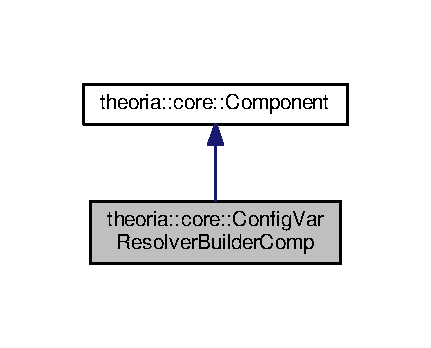
\includegraphics[width=207pt]{classtheoria_1_1core_1_1ConfigVarResolverBuilderComp__inherit__graph}
\end{center}
\end{figure}


Collaboration diagram for theoria\+:\+:core\+:\+:Config\+Var\+Resolver\+Builder\+Comp\+:
\nopagebreak
\begin{figure}[H]
\begin{center}
\leavevmode
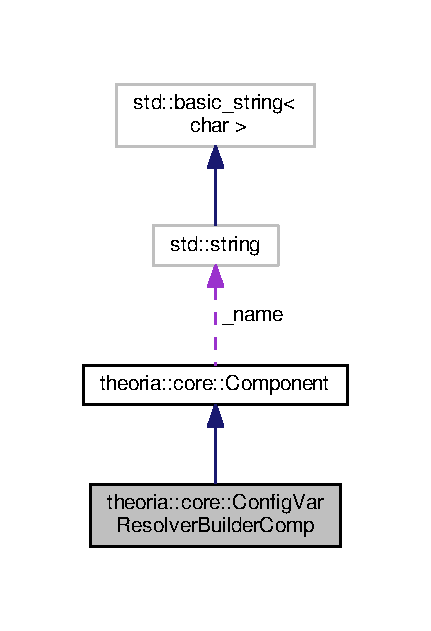
\includegraphics[width=350pt]{classtheoria_1_1core_1_1ConfigVarResolverBuilderComp__coll__graph}
\end{center}
\end{figure}
\subsection*{Public Member Functions}
\begin{DoxyCompactItemize}
\item 
\mbox{\Hypertarget{classtheoria_1_1core_1_1ConfigVarResolverBuilderComp_a14b04299b6eec3576e515ee204004df6}\label{classtheoria_1_1core_1_1ConfigVarResolverBuilderComp_a14b04299b6eec3576e515ee204004df6}} 
{\bfseries Config\+Var\+Resolver\+Builder\+Comp} (Comp\+Id id)
\item 
\hyperlink{classtheoria_1_1core_1_1Dependencies}{Dependencies} \hyperlink{classtheoria_1_1core_1_1ConfigVarResolverBuilderComp_aadf94c8b3d765667eaf9d7c91ac65342}{init} (const \hyperlink{classtheoria_1_1config_1_1Config}{config\+::\+Config} \&config) override
\item 
void \hyperlink{classtheoria_1_1core_1_1ConfigVarResolverBuilderComp_ac1e585a908c7e0fa7db4bdf0a8b514bb}{finalize} (const std\+::vector$<$ \hyperlink{classtheoria_1_1core_1_1Component}{Component} $\ast$$>$ \&dependencies) override
\item 
void \hyperlink{classtheoria_1_1core_1_1ConfigVarResolverBuilderComp_ad7d3e9f8ab3a2837526ffc3eda4c6c38}{app\+Life\+Cycle} (App\+Life\+Cycle state) override
\end{DoxyCompactItemize}
\subsection*{Static Public Member Functions}
\begin{DoxyCompactItemize}
\item 
\mbox{\Hypertarget{classtheoria_1_1core_1_1ConfigVarResolverBuilderComp_af290e5b8638b97e79d26a8d4597091ad}\label{classtheoria_1_1core_1_1ConfigVarResolverBuilderComp_af290e5b8638b97e79d26a8d4597091ad}} 
static \hyperlink{classtheoria_1_1core_1_1Component}{Component} $\ast$ {\bfseries factory} (Comp\+Id id)
\end{DoxyCompactItemize}
\subsection*{Static Public Attributes}
\begin{DoxyCompactItemize}
\item 
\mbox{\Hypertarget{classtheoria_1_1core_1_1ConfigVarResolverBuilderComp_ac80fd840a9280e471707d18c29557d9e}\label{classtheoria_1_1core_1_1ConfigVarResolverBuilderComp_ac80fd840a9280e471707d18c29557d9e}} 
static D\+L\+L\+\_\+\+P\+U\+B\+L\+IC \hyperlink{classtheoria_1_1core_1_1RegisterThis}{Register\+This}$<$ \hyperlink{classtheoria_1_1core_1_1ConfigVarResolverBuilderComp}{Config\+Var\+Resolver\+Builder\+Comp} $>$ {\bfseries rt}
\end{DoxyCompactItemize}
\subsection*{Additional Inherited Members}


\subsection{Member Function Documentation}
\mbox{\Hypertarget{classtheoria_1_1core_1_1ConfigVarResolverBuilderComp_ad7d3e9f8ab3a2837526ffc3eda4c6c38}\label{classtheoria_1_1core_1_1ConfigVarResolverBuilderComp_ad7d3e9f8ab3a2837526ffc3eda4c6c38}} 
\index{theoria\+::core\+::\+Config\+Var\+Resolver\+Builder\+Comp@{theoria\+::core\+::\+Config\+Var\+Resolver\+Builder\+Comp}!app\+Life\+Cycle@{app\+Life\+Cycle}}
\index{app\+Life\+Cycle@{app\+Life\+Cycle}!theoria\+::core\+::\+Config\+Var\+Resolver\+Builder\+Comp@{theoria\+::core\+::\+Config\+Var\+Resolver\+Builder\+Comp}}
\subsubsection{\texorpdfstring{app\+Life\+Cycle()}{appLifeCycle()}}
{\footnotesize\ttfamily void Config\+Var\+Resolver\+Builder\+Comp\+::app\+Life\+Cycle (\begin{DoxyParamCaption}\item[{App\+Life\+Cycle}]{state }\end{DoxyParamCaption})\hspace{0.3cm}{\ttfamily [override]}, {\ttfamily [virtual]}}

This is a place to take action on application lifecycle events. 

Reimplemented from \hyperlink{classtheoria_1_1core_1_1Component_ae036cde9b803a621149efeff7e0e00fc}{theoria\+::core\+::\+Component}.

\mbox{\Hypertarget{classtheoria_1_1core_1_1ConfigVarResolverBuilderComp_ac1e585a908c7e0fa7db4bdf0a8b514bb}\label{classtheoria_1_1core_1_1ConfigVarResolverBuilderComp_ac1e585a908c7e0fa7db4bdf0a8b514bb}} 
\index{theoria\+::core\+::\+Config\+Var\+Resolver\+Builder\+Comp@{theoria\+::core\+::\+Config\+Var\+Resolver\+Builder\+Comp}!finalize@{finalize}}
\index{finalize@{finalize}!theoria\+::core\+::\+Config\+Var\+Resolver\+Builder\+Comp@{theoria\+::core\+::\+Config\+Var\+Resolver\+Builder\+Comp}}
\subsubsection{\texorpdfstring{finalize()}{finalize()}}
{\footnotesize\ttfamily void Config\+Var\+Resolver\+Builder\+Comp\+::finalize (\begin{DoxyParamCaption}\item[{const std\+::vector$<$ \hyperlink{classtheoria_1_1core_1_1Component}{Component} $\ast$$>$ \&}]{dependencies }\end{DoxyParamCaption})\hspace{0.3cm}{\ttfamily [override]}, {\ttfamily [virtual]}}

The \hyperlink{classtheoria_1_1core_1_1ConfigVarResolverBuilderComp}{Config\+Var\+Resolver\+Builder\+Comp} job is to wire up Config\+Builder to chain of resolvers. 

Reimplemented from \hyperlink{classtheoria_1_1core_1_1Component_afd8acc89e2cd36e92bebe7e6fa530764}{theoria\+::core\+::\+Component}.

\mbox{\Hypertarget{classtheoria_1_1core_1_1ConfigVarResolverBuilderComp_aadf94c8b3d765667eaf9d7c91ac65342}\label{classtheoria_1_1core_1_1ConfigVarResolverBuilderComp_aadf94c8b3d765667eaf9d7c91ac65342}} 
\index{theoria\+::core\+::\+Config\+Var\+Resolver\+Builder\+Comp@{theoria\+::core\+::\+Config\+Var\+Resolver\+Builder\+Comp}!init@{init}}
\index{init@{init}!theoria\+::core\+::\+Config\+Var\+Resolver\+Builder\+Comp@{theoria\+::core\+::\+Config\+Var\+Resolver\+Builder\+Comp}}
\subsubsection{\texorpdfstring{init()}{init()}}
{\footnotesize\ttfamily \hyperlink{classtheoria_1_1core_1_1Dependencies}{Dependencies} Config\+Var\+Resolver\+Builder\+Comp\+::init (\begin{DoxyParamCaption}\item[{const \hyperlink{classtheoria_1_1config_1_1Config}{config\+::\+Config} \&}]{config }\end{DoxyParamCaption})\hspace{0.3cm}{\ttfamily [override]}, {\ttfamily [virtual]}}

Initialize component from its configuration and return the Components dependencies 

Reimplemented from \hyperlink{classtheoria_1_1core_1_1Component_a7ed45f6e38442a40666ae4556f794f7d}{theoria\+::core\+::\+Component}.



The documentation for this class was generated from the following files\+:\begin{DoxyCompactItemize}
\item 
include/theoria/core/Core\+Components.\+h\item 
src/core/Core\+Components.\+cpp\end{DoxyCompactItemize}

\hypertarget{classtheoria_1_1util_1_1densemap_1_1ConstIter}{\section{theoria\+:\+:util\+:\+:densemap$<$ K\+E\+Y, T, Alloc $>$\+:\+:Const\+Iter Class Reference}
\label{classtheoria_1_1util_1_1densemap_1_1ConstIter}\index{theoria\+::util\+::densemap$<$ K\+E\+Y, T, Alloc $>$\+::\+Const\+Iter@{theoria\+::util\+::densemap$<$ K\+E\+Y, T, Alloc $>$\+::\+Const\+Iter}}
}
\subsection*{Public Types}
\begin{DoxyCompactItemize}
\item 
\hypertarget{classtheoria_1_1util_1_1densemap_1_1ConstIter_a061fb76ecf5498d6033472fa66635d4a}{using {\bfseries value\+\_\+type} = std\+::pair$<$ K\+E\+Y, T $>$}\label{classtheoria_1_1util_1_1densemap_1_1ConstIter_a061fb76ecf5498d6033472fa66635d4a}

\end{DoxyCompactItemize}
\subsection*{Public Member Functions}
\begin{DoxyCompactItemize}
\item 
\hypertarget{classtheoria_1_1util_1_1densemap_1_1ConstIter_a41f22939ee0096d9d395f211fa757726}{{\bfseries Const\+Iter} (const \hyperlink{classtheoria_1_1util_1_1densemap_1_1ConstIter}{Const\+Iter} \&other)}\label{classtheoria_1_1util_1_1densemap_1_1ConstIter_a41f22939ee0096d9d395f211fa757726}

\item 
\hypertarget{classtheoria_1_1util_1_1densemap_1_1ConstIter_a393d12065a54dfadd07acb3268054695}{{\bfseries Const\+Iter} (typename Impl\+::const\+\_\+iterator iter, typename Impl\+::const\+\_\+iterator end)}\label{classtheoria_1_1util_1_1densemap_1_1ConstIter_a393d12065a54dfadd07acb3268054695}

\item 
\hypertarget{classtheoria_1_1util_1_1densemap_1_1ConstIter_a8c7a0c2774a2d4cb22aa82f83585dd27}{const \hyperlink{classtheoria_1_1util_1_1densemap_1_1ConstIter}{Const\+Iter} \& {\bfseries operator=} (const \hyperlink{classtheoria_1_1util_1_1densemap_1_1ConstIter}{Const\+Iter} \&other)}\label{classtheoria_1_1util_1_1densemap_1_1ConstIter_a8c7a0c2774a2d4cb22aa82f83585dd27}

\item 
\hypertarget{classtheoria_1_1util_1_1densemap_1_1ConstIter_ac53085842170c113e132f94477fc94a2}{bool {\bfseries operator==} (const \hyperlink{classtheoria_1_1util_1_1densemap_1_1ConstIter}{Const\+Iter} \&other) const }\label{classtheoria_1_1util_1_1densemap_1_1ConstIter_ac53085842170c113e132f94477fc94a2}

\item 
\hypertarget{classtheoria_1_1util_1_1densemap_1_1ConstIter_a28e3e50e698a6730d6465380e1f19d3c}{bool {\bfseries operator!=} (const \hyperlink{classtheoria_1_1util_1_1densemap_1_1ConstIter}{Const\+Iter} \&other) const }\label{classtheoria_1_1util_1_1densemap_1_1ConstIter_a28e3e50e698a6730d6465380e1f19d3c}

\item 
\hypertarget{classtheoria_1_1util_1_1densemap_1_1ConstIter_a354d30819cedb4921a95b6de2a3d02fe}{const value\+\_\+type \& {\bfseries operator$\ast$} () const }\label{classtheoria_1_1util_1_1densemap_1_1ConstIter_a354d30819cedb4921a95b6de2a3d02fe}

\item 
\hypertarget{classtheoria_1_1util_1_1densemap_1_1ConstIter_a8125b0eec84d2f34ec203b4f2cdddd51}{const value\+\_\+type $\ast$ {\bfseries operator-\/$>$} () const }\label{classtheoria_1_1util_1_1densemap_1_1ConstIter_a8125b0eec84d2f34ec203b4f2cdddd51}

\item 
\hypertarget{classtheoria_1_1util_1_1densemap_1_1ConstIter_a7dba18b534ffdf71354b4b5789aea3a1}{\hyperlink{classtheoria_1_1util_1_1densemap_1_1ConstIter}{Const\+Iter} {\bfseries operator++} ()}\label{classtheoria_1_1util_1_1densemap_1_1ConstIter_a7dba18b534ffdf71354b4b5789aea3a1}

\item 
\hypertarget{classtheoria_1_1util_1_1densemap_1_1ConstIter_a8ca98e8a181d846c7c8412192f59da95}{\hyperlink{classtheoria_1_1util_1_1densemap_1_1ConstIter}{Const\+Iter} {\bfseries operator++} (int)}\label{classtheoria_1_1util_1_1densemap_1_1ConstIter_a8ca98e8a181d846c7c8412192f59da95}

\end{DoxyCompactItemize}


The documentation for this class was generated from the following file\+:\begin{DoxyCompactItemize}
\item 
include/theoria/util/densemap.\+h\end{DoxyCompactItemize}

\hypertarget{classtheoria_1_1util_1_1densemap}{\section{theoria\+:\+:util\+:\+:densemap$<$ K\+E\+Y, T, Alloc $>$ Class Template Reference}
\label{classtheoria_1_1util_1_1densemap}\index{theoria\+::util\+::densemap$<$ K\+E\+Y, T, Alloc $>$@{theoria\+::util\+::densemap$<$ K\+E\+Y, T, Alloc $>$}}
}
\subsection*{Classes}
\begin{DoxyCompactItemize}
\item 
class \hyperlink{classtheoria_1_1util_1_1densemap_1_1ConstIter}{Const\+Iter}
\item 
class \hyperlink{classtheoria_1_1util_1_1densemap_1_1Iter}{Iter}
\end{DoxyCompactItemize}
\subsection*{Public Types}
\begin{DoxyCompactItemize}
\item 
\hypertarget{classtheoria_1_1util_1_1densemap_a133075e61db44e086c734c8a32ca6ab2}{using {\bfseries size\+\_\+type} = K\+E\+Y}\label{classtheoria_1_1util_1_1densemap_a133075e61db44e086c734c8a32ca6ab2}

\item 
\hypertarget{classtheoria_1_1util_1_1densemap_afd285a46dc8f45b4b1556a656708d2a7}{using {\bfseries key\+\_\+type} = K\+E\+Y}\label{classtheoria_1_1util_1_1densemap_afd285a46dc8f45b4b1556a656708d2a7}

\item 
\hypertarget{classtheoria_1_1util_1_1densemap_a8c1e5a57a1e76089bd675da3fa3347d8}{using {\bfseries mapped\+\_\+type} = T}\label{classtheoria_1_1util_1_1densemap_a8c1e5a57a1e76089bd675da3fa3347d8}

\item 
\hypertarget{classtheoria_1_1util_1_1densemap_a6d2419665695def56b2abbd849f74b08}{using {\bfseries value\+\_\+type} = std\+::pair$<$ K\+E\+Y, T $>$}\label{classtheoria_1_1util_1_1densemap_a6d2419665695def56b2abbd849f74b08}

\item 
\hypertarget{classtheoria_1_1util_1_1densemap_ae12f4688e504c8759e23759ad7272c94}{using {\bfseries allocator\+\_\+type} = Alloc}\label{classtheoria_1_1util_1_1densemap_ae12f4688e504c8759e23759ad7272c94}

\item 
\hypertarget{classtheoria_1_1util_1_1densemap_a20361bfcacef17947099d8580befbbdc}{using {\bfseries reference} = typename Alloc\+::reference}\label{classtheoria_1_1util_1_1densemap_a20361bfcacef17947099d8580befbbdc}

\item 
\hypertarget{classtheoria_1_1util_1_1densemap_a7a3dd11d6fd160c467c43d2029c3592a}{using {\bfseries const\+\_\+reference} = typename Alloc\+::const\+\_\+reference}\label{classtheoria_1_1util_1_1densemap_a7a3dd11d6fd160c467c43d2029c3592a}

\item 
\hypertarget{classtheoria_1_1util_1_1densemap_ae892a1fc35162971bb0278c7904995c6}{using {\bfseries pointer} = typename Alloc\+::pointer}\label{classtheoria_1_1util_1_1densemap_ae892a1fc35162971bb0278c7904995c6}

\item 
\hypertarget{classtheoria_1_1util_1_1densemap_ab19ebc07bf788b5689adaa3a80b46c31}{using {\bfseries const\+\_\+pointer} = typename Alloc\+::const\+\_\+pointer}\label{classtheoria_1_1util_1_1densemap_ab19ebc07bf788b5689adaa3a80b46c31}

\item 
\hypertarget{classtheoria_1_1util_1_1densemap_a4ee170442110252d3033534246f9677f}{using {\bfseries iterator} = \hyperlink{classtheoria_1_1util_1_1densemap_1_1Iter}{Iter}}\label{classtheoria_1_1util_1_1densemap_a4ee170442110252d3033534246f9677f}

\item 
\hypertarget{classtheoria_1_1util_1_1densemap_a8c2937f8e4ba47abf344d9f9f23f0c88}{using {\bfseries const\+\_\+iterator} = \hyperlink{classtheoria_1_1util_1_1densemap_1_1ConstIter}{Const\+Iter}}\label{classtheoria_1_1util_1_1densemap_a8c2937f8e4ba47abf344d9f9f23f0c88}

\end{DoxyCompactItemize}
\subsection*{Public Member Functions}
\begin{DoxyCompactItemize}
\item 
\hypertarget{classtheoria_1_1util_1_1densemap_a28dea7cc32d7cee72cf330bdf3e3201c}{{\bfseries densemap} (int n)}\label{classtheoria_1_1util_1_1densemap_a28dea7cc32d7cee72cf330bdf3e3201c}

\item 
\hypertarget{classtheoria_1_1util_1_1densemap_a4c32897f404f44c7de730637d09e18d5}{{\bfseries densemap} (allocator\+\_\+type alloc)}\label{classtheoria_1_1util_1_1densemap_a4c32897f404f44c7de730637d09e18d5}

\item 
\hypertarget{classtheoria_1_1util_1_1densemap_a8c6d546ba72e0516685424cb5c4c2467}{{\bfseries densemap} (const \hyperlink{classtheoria_1_1util_1_1densemap}{densemap} \&other)}\label{classtheoria_1_1util_1_1densemap_a8c6d546ba72e0516685424cb5c4c2467}

\item 
\hypertarget{classtheoria_1_1util_1_1densemap_ae8cbc01dc2418bffff40319a80df81e7}{{\bfseries densemap} (const \hyperlink{classtheoria_1_1util_1_1densemap}{densemap} \&other, allocator\+\_\+type alloc)}\label{classtheoria_1_1util_1_1densemap_ae8cbc01dc2418bffff40319a80df81e7}

\item 
\hypertarget{classtheoria_1_1util_1_1densemap_abd0a8736cb03cb0e4bbc7489a5274c78}{{\footnotesize template$<$typename Input\+Iter $>$ }\\{\bfseries densemap} (Input\+Iter first, Input\+Iter last)}\label{classtheoria_1_1util_1_1densemap_abd0a8736cb03cb0e4bbc7489a5274c78}

\item 
\hypertarget{classtheoria_1_1util_1_1densemap_a2fbff5aaf475fbd8492c9c766614517b}{{\bfseries densemap} (std\+::initializer\+\_\+list$<$ value\+\_\+type $>$ il, size\+\_\+type n=50)}\label{classtheoria_1_1util_1_1densemap_a2fbff5aaf475fbd8492c9c766614517b}

\item 
\hypertarget{classtheoria_1_1util_1_1densemap_a8205a6321acfcf7492c71c4912c348df}{mapped\+\_\+type {\bfseries at} (const key\+\_\+type \&key)}\label{classtheoria_1_1util_1_1densemap_a8205a6321acfcf7492c71c4912c348df}

\item 
\hypertarget{classtheoria_1_1util_1_1densemap_a511286991ffa72b606d52ae74668d5fe}{\hyperlink{classtheoria_1_1util_1_1densemap_1_1Iter}{iterator} {\bfseries begin} () noexcept}\label{classtheoria_1_1util_1_1densemap_a511286991ffa72b606d52ae74668d5fe}

\item 
\hypertarget{classtheoria_1_1util_1_1densemap_a602ddf67e5b8c1dc4459f71a0c7273b5}{\hyperlink{classtheoria_1_1util_1_1densemap_1_1ConstIter}{const\+\_\+iterator} {\bfseries begin} () const noexcept}\label{classtheoria_1_1util_1_1densemap_a602ddf67e5b8c1dc4459f71a0c7273b5}

\item 
\hypertarget{classtheoria_1_1util_1_1densemap_a2aebd517ccb28817684c62afc67396f3}{\hyperlink{classtheoria_1_1util_1_1densemap_1_1Iter}{iterator} {\bfseries end} () noexcept}\label{classtheoria_1_1util_1_1densemap_a2aebd517ccb28817684c62afc67396f3}

\item 
\hypertarget{classtheoria_1_1util_1_1densemap_a2f1d82722dd454f5804a28d76acc0986}{\hyperlink{classtheoria_1_1util_1_1densemap_1_1ConstIter}{const\+\_\+iterator} {\bfseries end} () const noexcept}\label{classtheoria_1_1util_1_1densemap_a2f1d82722dd454f5804a28d76acc0986}

\item 
\hypertarget{classtheoria_1_1util_1_1densemap_a10f53552f9f880393cad9085ff9d5a23}{size\+\_\+type {\bfseries bucket} (const key\+\_\+type \&key) const noexcept}\label{classtheoria_1_1util_1_1densemap_a10f53552f9f880393cad9085ff9d5a23}

\item 
\hypertarget{classtheoria_1_1util_1_1densemap_acb06213b8d862b1295c79752a2329fd6}{size\+\_\+type {\bfseries bucket\+\_\+count} () const noexcept}\label{classtheoria_1_1util_1_1densemap_acb06213b8d862b1295c79752a2329fd6}

\item 
\hypertarget{classtheoria_1_1util_1_1densemap_a4e82874d3fe3d61d5e9a9f7405531316}{size\+\_\+type {\bfseries bucket\+\_\+size} () const noexcept}\label{classtheoria_1_1util_1_1densemap_a4e82874d3fe3d61d5e9a9f7405531316}

\item 
\hypertarget{classtheoria_1_1util_1_1densemap_a519f986513c0242d89cb97a36b587743}{\hyperlink{classtheoria_1_1util_1_1densemap_1_1ConstIter}{const\+\_\+iterator} {\bfseries cbegin} () const noexcept}\label{classtheoria_1_1util_1_1densemap_a519f986513c0242d89cb97a36b587743}

\item 
\hypertarget{classtheoria_1_1util_1_1densemap_a01965a6fe934583b09cb0812e673d64c}{\hyperlink{classtheoria_1_1util_1_1densemap_1_1ConstIter}{const\+\_\+iterator} {\bfseries cend} () const noexcept}\label{classtheoria_1_1util_1_1densemap_a01965a6fe934583b09cb0812e673d64c}

\item 
\hypertarget{classtheoria_1_1util_1_1densemap_ae087d2be9f5947d79522f6a3b592786e}{void {\bfseries clear} () noexcept}\label{classtheoria_1_1util_1_1densemap_ae087d2be9f5947d79522f6a3b592786e}

\item 
\hypertarget{classtheoria_1_1util_1_1densemap_ad06bf0be6b547e08f57588c78cc8b3f6}{size\+\_\+t {\bfseries count} (const key\+\_\+type \&k) const noexcept}\label{classtheoria_1_1util_1_1densemap_ad06bf0be6b547e08f57588c78cc8b3f6}

\item 
\hypertarget{classtheoria_1_1util_1_1densemap_aff92774c3fb8a22bef1178348845304f}{bool {\bfseries empty} () const noexcept}\label{classtheoria_1_1util_1_1densemap_aff92774c3fb8a22bef1178348845304f}

\item 
\hypertarget{classtheoria_1_1util_1_1densemap_acf76f330db3de660d40b624c18f92f4c}{\hyperlink{classtheoria_1_1util_1_1densemap_1_1Iter}{iterator} {\bfseries find} (const key\+\_\+type \&k)}\label{classtheoria_1_1util_1_1densemap_acf76f330db3de660d40b624c18f92f4c}

\item 
\hypertarget{classtheoria_1_1util_1_1densemap_aaa6c471543fe77af8eea0a06476bc7b5}{\hyperlink{classtheoria_1_1util_1_1densemap_1_1ConstIter}{const\+\_\+iterator} {\bfseries find} (const key\+\_\+type \&k) const }\label{classtheoria_1_1util_1_1densemap_aaa6c471543fe77af8eea0a06476bc7b5}

\item 
\hypertarget{classtheoria_1_1util_1_1densemap_a10d1d4e2e83bab6062f12b63ed78146d}{std\+::pair$<$ \hyperlink{classtheoria_1_1util_1_1densemap_1_1Iter}{iterator}, bool $>$ {\bfseries insert} (value\+\_\+type \&val)}\label{classtheoria_1_1util_1_1densemap_a10d1d4e2e83bab6062f12b63ed78146d}

\item 
\hypertarget{classtheoria_1_1util_1_1densemap_a3d482d15fc6ea59df3b04d5672aa22de}{size\+\_\+t {\bfseries size} () const noexcept}\label{classtheoria_1_1util_1_1densemap_a3d482d15fc6ea59df3b04d5672aa22de}

\item 
\hypertarget{classtheoria_1_1util_1_1densemap_a98cd543bdf981a2a199f6aaf7e0db02d}{mapped\+\_\+type \& {\bfseries operator\mbox{[}$\,$\mbox{]}} (const key\+\_\+type \&k)}\label{classtheoria_1_1util_1_1densemap_a98cd543bdf981a2a199f6aaf7e0db02d}

\item 
\hypertarget{classtheoria_1_1util_1_1densemap_abf66875d894d9a0a8b40c9d4ab9aed76}{const mapped\+\_\+type \& {\bfseries operator\mbox{[}$\,$\mbox{]}} (const key\+\_\+type \&k) const }\label{classtheoria_1_1util_1_1densemap_abf66875d894d9a0a8b40c9d4ab9aed76}

\item 
\hypertarget{classtheoria_1_1util_1_1densemap_aa7556f5cea18d37c8ecacd6907742020}{mapped\+\_\+type \& {\bfseries operator\mbox{[}$\,$\mbox{]}} (key\+\_\+type \&\&k)}\label{classtheoria_1_1util_1_1densemap_aa7556f5cea18d37c8ecacd6907742020}

\item 
\hypertarget{classtheoria_1_1util_1_1densemap_a9ca5e32347009b58c2c225ee37cbc0fa}{key\+\_\+type {\bfseries add} (mapped\+\_\+type value)}\label{classtheoria_1_1util_1_1densemap_a9ca5e32347009b58c2c225ee37cbc0fa}

\end{DoxyCompactItemize}


The documentation for this class was generated from the following file\+:\begin{DoxyCompactItemize}
\item 
include/theoria/util/densemap.\+h\end{DoxyCompactItemize}

\hypertarget{classtheoria_1_1core_1_1Dependencies}{}\section{theoria\+:\+:core\+:\+:Dependencies Class Reference}
\label{classtheoria_1_1core_1_1Dependencies}\index{theoria\+::core\+::\+Dependencies@{theoria\+::core\+::\+Dependencies}}
\subsection*{Classes}
\begin{DoxyCompactItemize}
\item 
struct \hyperlink{structtheoria_1_1core_1_1Dependencies_1_1Dependent}{Dependent}
\end{DoxyCompactItemize}
\subsection*{Public Types}
\begin{DoxyCompactItemize}
\item 
\mbox{\Hypertarget{classtheoria_1_1core_1_1Dependencies_af58b879e807df8fb52b96c9ab1eb6073}\label{classtheoria_1_1core_1_1Dependencies_af58b879e807df8fb52b96c9ab1eb6073}} 
using {\bfseries const\+\_\+iterator} = Deps\+List\+::const\+\_\+iterator
\end{DoxyCompactItemize}
\subsection*{Public Member Functions}
\begin{DoxyCompactItemize}
\item 
\mbox{\Hypertarget{classtheoria_1_1core_1_1Dependencies_a71b275a54e4261724540c60818d4ef85}\label{classtheoria_1_1core_1_1Dependencies_a71b275a54e4261724540c60818d4ef85}} 
{\bfseries Dependencies} (\hyperlink{classtheoria_1_1core_1_1Dependencies}{Dependencies} \&\&other) noexcept
\item 
\mbox{\Hypertarget{classtheoria_1_1core_1_1Dependencies_ad3f8a71bd7ce6ff9e244d7072eb030e7}\label{classtheoria_1_1core_1_1Dependencies_ad3f8a71bd7ce6ff9e244d7072eb030e7}} 
{\bfseries Dependencies} (const \hyperlink{classtheoria_1_1core_1_1Dependencies}{Dependencies} \&other) noexcept
\item 
\mbox{\Hypertarget{classtheoria_1_1core_1_1Dependencies_ac1b06e338d69428c95de7851dfc43935}\label{classtheoria_1_1core_1_1Dependencies_ac1b06e338d69428c95de7851dfc43935}} 
\hyperlink{classtheoria_1_1core_1_1Dependencies}{Dependencies} \& {\bfseries operator=} (\hyperlink{classtheoria_1_1core_1_1Dependencies}{Dependencies} \&\&other)=default
\item 
\mbox{\Hypertarget{classtheoria_1_1core_1_1Dependencies_ac0c7b2c350c5e904732ed07b13852c21}\label{classtheoria_1_1core_1_1Dependencies_ac0c7b2c350c5e904732ed07b13852c21}} 
\hyperlink{classtheoria_1_1core_1_1Dependencies}{Dependencies} \& {\bfseries operator=} (\hyperlink{classtheoria_1_1core_1_1Dependencies}{Dependencies} \&other)=default
\item 
\hyperlink{classtheoria_1_1core_1_1Dependencies}{Dependencies} \& \hyperlink{classtheoria_1_1core_1_1Dependencies_afa22a8f9fc20d3ce417bac397ba22e7a}{loose} (const Type\+Name \&type, bool optional=false)
\item 
\hyperlink{classtheoria_1_1core_1_1Dependencies}{Dependencies} \& \hyperlink{classtheoria_1_1core_1_1Dependencies_ae3995847906cda98292e0a9215797d41}{def} (const Type\+Name \&name, bool optional=false)
\item 
\hyperlink{classtheoria_1_1core_1_1Dependencies}{Dependencies} \& \hyperlink{classtheoria_1_1core_1_1Dependencies_a7daeed943359e4290cbdcf6d0c3c57b5}{strict} (const Type\+Name \&type, const Sub\+Type\+Name \&name, bool optional=false)
\item 
\mbox{\Hypertarget{classtheoria_1_1core_1_1Dependencies_a830f5b83a926234ace464e441670974b}\label{classtheoria_1_1core_1_1Dependencies_a830f5b83a926234ace464e441670974b}} 
const\+\_\+iterator {\bfseries begin} () const
\item 
\mbox{\Hypertarget{classtheoria_1_1core_1_1Dependencies_ae1acd1d0962abda73cb1a46447dd4a5e}\label{classtheoria_1_1core_1_1Dependencies_ae1acd1d0962abda73cb1a46447dd4a5e}} 
const\+\_\+iterator {\bfseries end} () const
\item 
\mbox{\Hypertarget{classtheoria_1_1core_1_1Dependencies_a5d099bcbccf7ae14e5a373aa6be82288}\label{classtheoria_1_1core_1_1Dependencies_a5d099bcbccf7ae14e5a373aa6be82288}} 
int {\bfseries size} () const
\item 
\mbox{\Hypertarget{classtheoria_1_1core_1_1Dependencies_afba2a36945b9320b793ff8f3350ce468}\label{classtheoria_1_1core_1_1Dependencies_afba2a36945b9320b793ff8f3350ce468}} 
const \hyperlink{structtheoria_1_1core_1_1Dependencies_1_1Dependent}{Dependent} \& {\bfseries operator\mbox{[}$\,$\mbox{]}} (int idx) const
\end{DoxyCompactItemize}
\subsection*{Friends}
\begin{DoxyCompactItemize}
\item 
\mbox{\Hypertarget{classtheoria_1_1core_1_1Dependencies_a3fef4fe6d625d0698807b631fa90db4b}\label{classtheoria_1_1core_1_1Dependencies_a3fef4fe6d625d0698807b631fa90db4b}} 
bool {\bfseries operator==} (const \hyperlink{classtheoria_1_1core_1_1Dependencies}{Dependencies} \&a, const \hyperlink{classtheoria_1_1core_1_1Dependencies}{Dependencies} \&b)
\end{DoxyCompactItemize}


\subsection{Member Function Documentation}
\mbox{\Hypertarget{classtheoria_1_1core_1_1Dependencies_ae3995847906cda98292e0a9215797d41}\label{classtheoria_1_1core_1_1Dependencies_ae3995847906cda98292e0a9215797d41}} 
\index{theoria\+::core\+::\+Dependencies@{theoria\+::core\+::\+Dependencies}!def@{def}}
\index{def@{def}!theoria\+::core\+::\+Dependencies@{theoria\+::core\+::\+Dependencies}}
\subsubsection{\texorpdfstring{def()}{def()}}
{\footnotesize\ttfamily \hyperlink{classtheoria_1_1core_1_1Dependencies}{Dependencies}\& theoria\+::core\+::\+Dependencies\+::def (\begin{DoxyParamCaption}\item[{const Type\+Name \&}]{name,  }\item[{bool}]{optional = {\ttfamily false} }\end{DoxyParamCaption})\hspace{0.3cm}{\ttfamily [inline]}}

Add a dependent to a component of the given type such that the type matches it\textquotesingle{}s subtype . Such a component can be thought of as the default component of that type and there can be only 0 or 1. \mbox{\Hypertarget{classtheoria_1_1core_1_1Dependencies_afa22a8f9fc20d3ce417bac397ba22e7a}\label{classtheoria_1_1core_1_1Dependencies_afa22a8f9fc20d3ce417bac397ba22e7a}} 
\index{theoria\+::core\+::\+Dependencies@{theoria\+::core\+::\+Dependencies}!loose@{loose}}
\index{loose@{loose}!theoria\+::core\+::\+Dependencies@{theoria\+::core\+::\+Dependencies}}
\subsubsection{\texorpdfstring{loose()}{loose()}}
{\footnotesize\ttfamily \hyperlink{classtheoria_1_1core_1_1Dependencies}{Dependencies}\& theoria\+::core\+::\+Dependencies\+::loose (\begin{DoxyParamCaption}\item[{const Type\+Name \&}]{type,  }\item[{bool}]{optional = {\ttfamily false} }\end{DoxyParamCaption})\hspace{0.3cm}{\ttfamily [inline]}}

Add a dependent to a component of the given type. If there are multiple components of this type it will pick the first one that has existing dependencies otherwise the first one it sees. \mbox{\Hypertarget{classtheoria_1_1core_1_1Dependencies_a7daeed943359e4290cbdcf6d0c3c57b5}\label{classtheoria_1_1core_1_1Dependencies_a7daeed943359e4290cbdcf6d0c3c57b5}} 
\index{theoria\+::core\+::\+Dependencies@{theoria\+::core\+::\+Dependencies}!strict@{strict}}
\index{strict@{strict}!theoria\+::core\+::\+Dependencies@{theoria\+::core\+::\+Dependencies}}
\subsubsection{\texorpdfstring{strict()}{strict()}}
{\footnotesize\ttfamily \hyperlink{classtheoria_1_1core_1_1Dependencies}{Dependencies}\& theoria\+::core\+::\+Dependencies\+::strict (\begin{DoxyParamCaption}\item[{const Type\+Name \&}]{type,  }\item[{const Sub\+Type\+Name \&}]{name,  }\item[{bool}]{optional = {\ttfamily false} }\end{DoxyParamCaption})\hspace{0.3cm}{\ttfamily [inline]}}

Add a dependent with the specified type and subtype. There can be only 0 or 1. This is a strict dependency because the dependent is anouncing that one and only one implementation will do 

The documentation for this class was generated from the following file\+:\begin{DoxyCompactItemize}
\item 
include/theoria/core/Dependencies.\+h\end{DoxyCompactItemize}

\hypertarget{structtheoria_1_1core_1_1Dependencies_1_1Dependent}{\section{theoria\+:\+:core\+:\+:Dependencies\+:\+:Dependent Struct Reference}
\label{structtheoria_1_1core_1_1Dependencies_1_1Dependent}\index{theoria\+::core\+::\+Dependencies\+::\+Dependent@{theoria\+::core\+::\+Dependencies\+::\+Dependent}}
}


Collaboration diagram for theoria\+:\+:core\+:\+:Dependencies\+:\+:Dependent\+:
\nopagebreak
\begin{figure}[H]
\begin{center}
\leavevmode
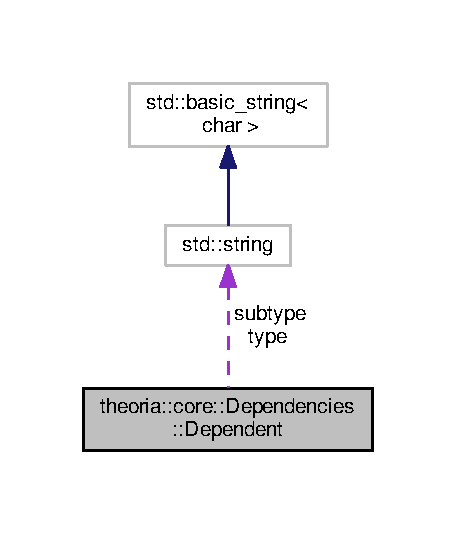
\includegraphics[width=219pt]{structtheoria_1_1core_1_1Dependencies_1_1Dependent__coll__graph}
\end{center}
\end{figure}
\subsection*{Public Member Functions}
\begin{DoxyCompactItemize}
\item 
\hypertarget{structtheoria_1_1core_1_1Dependencies_1_1Dependent_a25a03961885377f8d61f235968de9d7a}{{\bfseries Dependent} (const Type\+Name \&type\+\_\+, const Sub\+Type\+Name \&subtype\+\_\+, int optional\+\_\+=false)}\label{structtheoria_1_1core_1_1Dependencies_1_1Dependent_a25a03961885377f8d61f235968de9d7a}

\item 
\hypertarget{structtheoria_1_1core_1_1Dependencies_1_1Dependent_ac2d4b0f74da74e8e8b33690354a4c245}{{\bfseries Dependent} (const Type\+Name \&type\+\_\+, int optional\+\_\+=false)}\label{structtheoria_1_1core_1_1Dependencies_1_1Dependent_ac2d4b0f74da74e8e8b33690354a4c245}

\item 
\hypertarget{structtheoria_1_1core_1_1Dependencies_1_1Dependent_a2718fb0114fe1f185051bfb35d441518}{bool {\bfseries required} () const }\label{structtheoria_1_1core_1_1Dependencies_1_1Dependent_a2718fb0114fe1f185051bfb35d441518}

\item 
\hypertarget{structtheoria_1_1core_1_1Dependencies_1_1Dependent_a2226eeac97d0b57bfdeaed91442cdc86}{std\+::string {\bfseries str} () const }\label{structtheoria_1_1core_1_1Dependencies_1_1Dependent_a2226eeac97d0b57bfdeaed91442cdc86}

\item 
\hypertarget{structtheoria_1_1core_1_1Dependencies_1_1Dependent_ac6116c1e0f4083636db2f170d8cd1938}{{\bfseries operator std\+::string} ()}\label{structtheoria_1_1core_1_1Dependencies_1_1Dependent_ac6116c1e0f4083636db2f170d8cd1938}

\end{DoxyCompactItemize}
\subsection*{Public Attributes}
\begin{DoxyCompactItemize}
\item 
\hypertarget{structtheoria_1_1core_1_1Dependencies_1_1Dependent_a9a4198c7cffacace0d8971a6ae5536b3}{Type\+Name {\bfseries type}}\label{structtheoria_1_1core_1_1Dependencies_1_1Dependent_a9a4198c7cffacace0d8971a6ae5536b3}

\item 
\hypertarget{structtheoria_1_1core_1_1Dependencies_1_1Dependent_a2748915ec9980f392a2092b4bc1c3a1a}{Sub\+Type\+Name {\bfseries subtype}}\label{structtheoria_1_1core_1_1Dependencies_1_1Dependent_a2748915ec9980f392a2092b4bc1c3a1a}

\item 
\hypertarget{structtheoria_1_1core_1_1Dependencies_1_1Dependent_a81f5f761e3b6b5db488126b909d60601}{bool {\bfseries optional}}\label{structtheoria_1_1core_1_1Dependencies_1_1Dependent_a81f5f761e3b6b5db488126b909d60601}

\end{DoxyCompactItemize}


The documentation for this struct was generated from the following files\+:\begin{DoxyCompactItemize}
\item 
include/theoria/core/Dependencies.\+h\item 
src/core/Dependencies.\+cpp\end{DoxyCompactItemize}

\hypertarget{classtheoria_1_1config_1_1DisableResolver}{}\section{theoria\+:\+:config\+:\+:Disable\+Resolver Class Reference}
\label{classtheoria_1_1config_1_1DisableResolver}\index{theoria\+::config\+::\+Disable\+Resolver@{theoria\+::config\+::\+Disable\+Resolver}}


Inheritance diagram for theoria\+:\+:config\+:\+:Disable\+Resolver\+:
\nopagebreak
\begin{figure}[H]
\begin{center}
\leavevmode
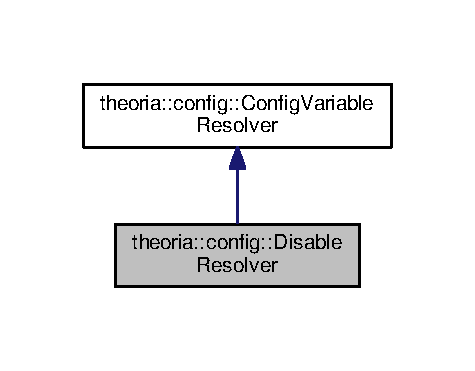
\includegraphics[width=228pt]{classtheoria_1_1config_1_1DisableResolver__inherit__graph}
\end{center}
\end{figure}


Collaboration diagram for theoria\+:\+:config\+:\+:Disable\+Resolver\+:
\nopagebreak
\begin{figure}[H]
\begin{center}
\leavevmode
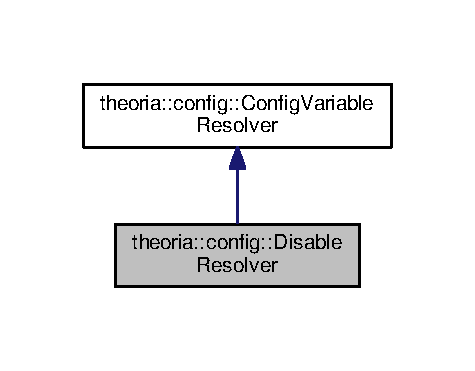
\includegraphics[width=228pt]{classtheoria_1_1config_1_1DisableResolver__coll__graph}
\end{center}
\end{figure}
\subsection*{Public Member Functions}
\begin{DoxyCompactItemize}
\item 
\mbox{\Hypertarget{classtheoria_1_1config_1_1DisableResolver_ae366903d552dd3a34a380e4918525cd1}\label{classtheoria_1_1config_1_1DisableResolver_ae366903d552dd3a34a380e4918525cd1}} 
Result {\bfseries lookup} (const std\+::string \&\hyperlink{classtheoria_1_1config_1_1DisableResolver_ae7caa7a59ad2921ec2cba0544ed26ad0}{name}) const override
\item 
virtual std\+::string \hyperlink{classtheoria_1_1config_1_1DisableResolver_ae7caa7a59ad2921ec2cba0544ed26ad0}{name} () const override
\end{DoxyCompactItemize}
\subsection*{Additional Inherited Members}


\subsection{Member Function Documentation}
\mbox{\Hypertarget{classtheoria_1_1config_1_1DisableResolver_ae7caa7a59ad2921ec2cba0544ed26ad0}\label{classtheoria_1_1config_1_1DisableResolver_ae7caa7a59ad2921ec2cba0544ed26ad0}} 
\index{theoria\+::config\+::\+Disable\+Resolver@{theoria\+::config\+::\+Disable\+Resolver}!name@{name}}
\index{name@{name}!theoria\+::config\+::\+Disable\+Resolver@{theoria\+::config\+::\+Disable\+Resolver}}
\subsubsection{\texorpdfstring{name()}{name()}}
{\footnotesize\ttfamily std\+::string Disable\+Resolver\+::name (\begin{DoxyParamCaption}{ }\end{DoxyParamCaption}) const\hspace{0.3cm}{\ttfamily [override]}, {\ttfamily [virtual]}}

Return name of the resolver 

Implements \hyperlink{classtheoria_1_1config_1_1ConfigVariableResolver_a026bda729faf988eaef334a45ec92303}{theoria\+::config\+::\+Config\+Variable\+Resolver}.



The documentation for this class was generated from the following files\+:\begin{DoxyCompactItemize}
\item 
include/theoria/config/Resolve.\+h\item 
src/config/Resolve.\+cpp\end{DoxyCompactItemize}

\hypertarget{classtheoria_1_1config_1_1DisallowResolver}{}\section{theoria\+:\+:config\+:\+:Disallow\+Resolver Class Reference}
\label{classtheoria_1_1config_1_1DisallowResolver}\index{theoria\+::config\+::\+Disallow\+Resolver@{theoria\+::config\+::\+Disallow\+Resolver}}


Inheritance diagram for theoria\+:\+:config\+:\+:Disallow\+Resolver\+:
\nopagebreak
\begin{figure}[H]
\begin{center}
\leavevmode
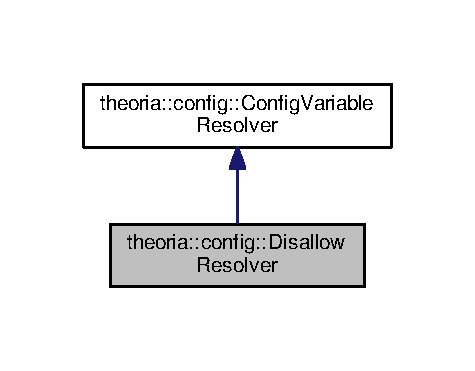
\includegraphics[width=228pt]{classtheoria_1_1config_1_1DisallowResolver__inherit__graph}
\end{center}
\end{figure}


Collaboration diagram for theoria\+:\+:config\+:\+:Disallow\+Resolver\+:
\nopagebreak
\begin{figure}[H]
\begin{center}
\leavevmode
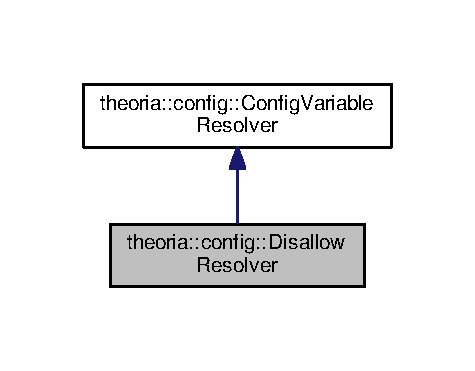
\includegraphics[width=228pt]{classtheoria_1_1config_1_1DisallowResolver__coll__graph}
\end{center}
\end{figure}
\subsection*{Public Member Functions}
\begin{DoxyCompactItemize}
\item 
\mbox{\Hypertarget{classtheoria_1_1config_1_1DisallowResolver_a70db68fce5348edea51d7303f2bb3f33}\label{classtheoria_1_1config_1_1DisallowResolver_a70db68fce5348edea51d7303f2bb3f33}} 
Result {\bfseries lookup} (const std\+::string \&\hyperlink{classtheoria_1_1config_1_1DisallowResolver_a8352df79f9e0f17fbfad8801bfdcc99e}{name}) const override
\item 
virtual std\+::string \hyperlink{classtheoria_1_1config_1_1DisallowResolver_a8352df79f9e0f17fbfad8801bfdcc99e}{name} () const override
\end{DoxyCompactItemize}
\subsection*{Additional Inherited Members}


\subsection{Member Function Documentation}
\mbox{\Hypertarget{classtheoria_1_1config_1_1DisallowResolver_a8352df79f9e0f17fbfad8801bfdcc99e}\label{classtheoria_1_1config_1_1DisallowResolver_a8352df79f9e0f17fbfad8801bfdcc99e}} 
\index{theoria\+::config\+::\+Disallow\+Resolver@{theoria\+::config\+::\+Disallow\+Resolver}!name@{name}}
\index{name@{name}!theoria\+::config\+::\+Disallow\+Resolver@{theoria\+::config\+::\+Disallow\+Resolver}}
\subsubsection{\texorpdfstring{name()}{name()}}
{\footnotesize\ttfamily std\+::string Disallow\+Resolver\+::name (\begin{DoxyParamCaption}{ }\end{DoxyParamCaption}) const\hspace{0.3cm}{\ttfamily [override]}, {\ttfamily [virtual]}}

Return name of the resolver 

Implements \hyperlink{classtheoria_1_1config_1_1ConfigVariableResolver_a026bda729faf988eaef334a45ec92303}{theoria\+::config\+::\+Config\+Variable\+Resolver}.



The documentation for this class was generated from the following files\+:\begin{DoxyCompactItemize}
\item 
include/theoria/config/Resolve.\+h\item 
src/config/Resolve.\+cpp\end{DoxyCompactItemize}

\hypertarget{classtheoria_1_1config_1_1EnvVarResolver}{}\section{theoria\+:\+:config\+:\+:Env\+Var\+Resolver Class Reference}
\label{classtheoria_1_1config_1_1EnvVarResolver}\index{theoria\+::config\+::\+Env\+Var\+Resolver@{theoria\+::config\+::\+Env\+Var\+Resolver}}


{\ttfamily \#include $<$Resolve.\+h$>$}



Inheritance diagram for theoria\+:\+:config\+:\+:Env\+Var\+Resolver\+:\nopagebreak
\begin{figure}[H]
\begin{center}
\leavevmode
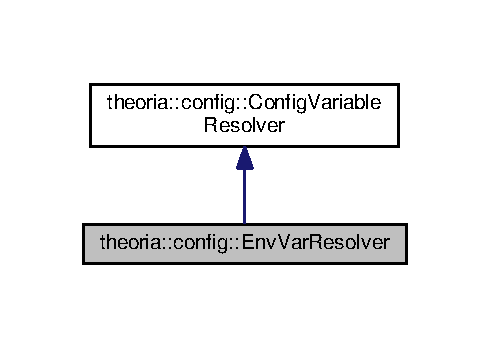
\includegraphics[width=235pt]{classtheoria_1_1config_1_1EnvVarResolver__inherit__graph}
\end{center}
\end{figure}


Collaboration diagram for theoria\+:\+:config\+:\+:Env\+Var\+Resolver\+:\nopagebreak
\begin{figure}[H]
\begin{center}
\leavevmode
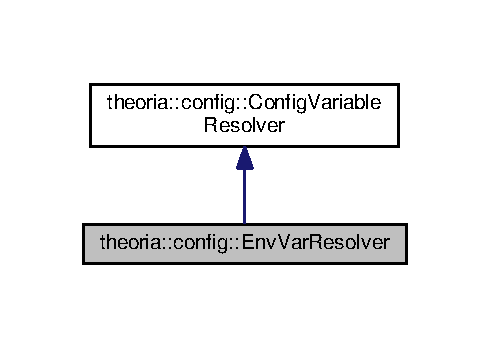
\includegraphics[width=235pt]{classtheoria_1_1config_1_1EnvVarResolver__coll__graph}
\end{center}
\end{figure}
\subsection*{Public Member Functions}
\begin{DoxyCompactItemize}
\item 
\hyperlink{classtheoria_1_1config_1_1ConfigVariableResolver_af27a85262d802c9ad4ecb1179efaf447}{Result} \hyperlink{classtheoria_1_1config_1_1EnvVarResolver_abe8584760283bca6c2ebda1116c8159b}{lookup} (const std\+::string \&\hyperlink{classtheoria_1_1config_1_1EnvVarResolver_ab2c250e1b7866dcd618dc90f3c3eab19}{name}) const override
\item 
virtual std\+::string \hyperlink{classtheoria_1_1config_1_1EnvVarResolver_ab2c250e1b7866dcd618dc90f3c3eab19}{name} () const override
\end{DoxyCompactItemize}
\subsection*{Additional Inherited Members}


\subsection{Detailed Description}
Resolves variables from the os environment 

\subsection{Member Function Documentation}
\mbox{\Hypertarget{classtheoria_1_1config_1_1EnvVarResolver_abe8584760283bca6c2ebda1116c8159b}\label{classtheoria_1_1config_1_1EnvVarResolver_abe8584760283bca6c2ebda1116c8159b}} 
\index{theoria\+::config\+::\+Env\+Var\+Resolver@{theoria\+::config\+::\+Env\+Var\+Resolver}!lookup@{lookup}}
\index{lookup@{lookup}!theoria\+::config\+::\+Env\+Var\+Resolver@{theoria\+::config\+::\+Env\+Var\+Resolver}}
\subsubsection{\texorpdfstring{lookup()}{lookup()}}
{\footnotesize\ttfamily \hyperlink{classtheoria_1_1config_1_1ConfigVariableResolver_af27a85262d802c9ad4ecb1179efaf447}{Result} Env\+Var\+Resolver\+::lookup (\begin{DoxyParamCaption}\item[{const std\+::string \&}]{name }\end{DoxyParamCaption}) const\hspace{0.3cm}{\ttfamily [override]}, {\ttfamily [virtual]}}

Resolve name by looking at env variable with same name 

Implements \hyperlink{classtheoria_1_1config_1_1ConfigVariableResolver}{theoria\+::config\+::\+Config\+Variable\+Resolver}.

\mbox{\Hypertarget{classtheoria_1_1config_1_1EnvVarResolver_ab2c250e1b7866dcd618dc90f3c3eab19}\label{classtheoria_1_1config_1_1EnvVarResolver_ab2c250e1b7866dcd618dc90f3c3eab19}} 
\index{theoria\+::config\+::\+Env\+Var\+Resolver@{theoria\+::config\+::\+Env\+Var\+Resolver}!name@{name}}
\index{name@{name}!theoria\+::config\+::\+Env\+Var\+Resolver@{theoria\+::config\+::\+Env\+Var\+Resolver}}
\subsubsection{\texorpdfstring{name()}{name()}}
{\footnotesize\ttfamily std\+::string Env\+Var\+Resolver\+::name (\begin{DoxyParamCaption}{ }\end{DoxyParamCaption}) const\hspace{0.3cm}{\ttfamily [override]}, {\ttfamily [virtual]}}

Returns \char`\"{}\+Env\+Var\+Resolver\char`\"{} 

Implements \hyperlink{classtheoria_1_1config_1_1ConfigVariableResolver_a026bda729faf988eaef334a45ec92303}{theoria\+::config\+::\+Config\+Variable\+Resolver}.



The documentation for this class was generated from the following files\+:\begin{DoxyCompactItemize}
\item 
include/theoria/config/Resolve.\+h\item 
src/config/Resolve.\+cpp\end{DoxyCompactItemize}

\hypertarget{classtheoria_1_1core_1_1EnvVarResolverComp}{}\section{theoria\+:\+:core\+:\+:Env\+Var\+Resolver\+Comp Class Reference}
\label{classtheoria_1_1core_1_1EnvVarResolverComp}\index{theoria\+::core\+::\+Env\+Var\+Resolver\+Comp@{theoria\+::core\+::\+Env\+Var\+Resolver\+Comp}}


Inheritance diagram for theoria\+:\+:core\+:\+:Env\+Var\+Resolver\+Comp\+:
\nopagebreak
\begin{figure}[H]
\begin{center}
\leavevmode
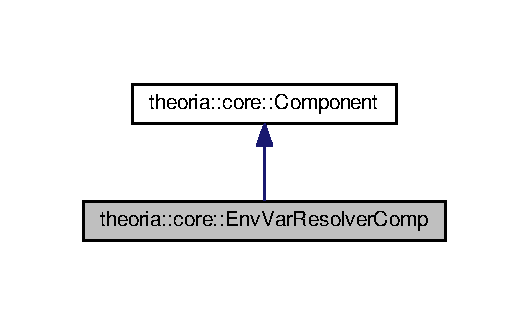
\includegraphics[width=254pt]{classtheoria_1_1core_1_1EnvVarResolverComp__inherit__graph}
\end{center}
\end{figure}


Collaboration diagram for theoria\+:\+:core\+:\+:Env\+Var\+Resolver\+Comp\+:
\nopagebreak
\begin{figure}[H]
\begin{center}
\leavevmode
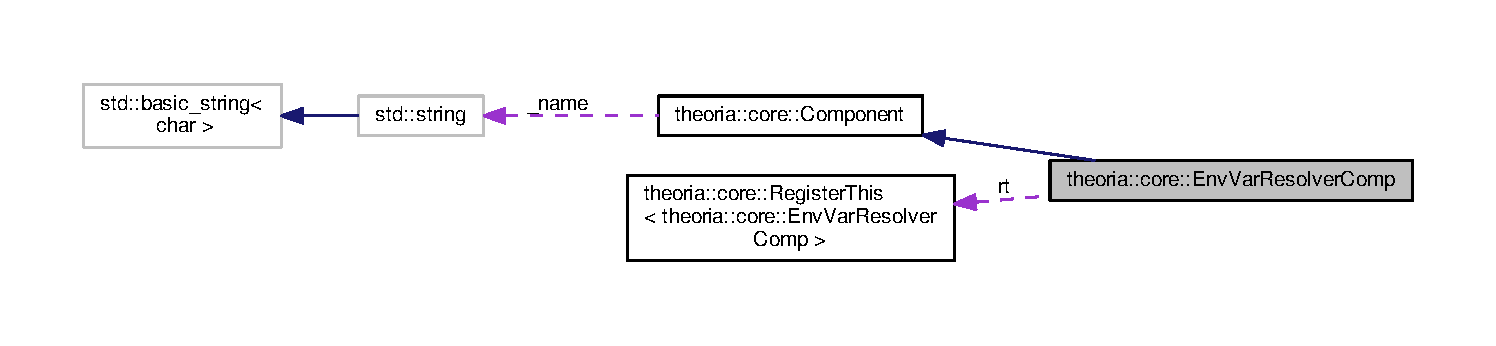
\includegraphics[width=350pt]{classtheoria_1_1core_1_1EnvVarResolverComp__coll__graph}
\end{center}
\end{figure}
\subsection*{Public Member Functions}
\begin{DoxyCompactItemize}
\item 
\mbox{\Hypertarget{classtheoria_1_1core_1_1EnvVarResolverComp_a0d015c8dd5ad4e8f2b1e33af88f0791a}\label{classtheoria_1_1core_1_1EnvVarResolverComp_a0d015c8dd5ad4e8f2b1e33af88f0791a}} 
{\bfseries Env\+Var\+Resolver\+Comp} (Comp\+Id id)
\item 
\mbox{\Hypertarget{classtheoria_1_1core_1_1EnvVarResolverComp_aac22e843f14123d2627f8c8ca0311b80}\label{classtheoria_1_1core_1_1EnvVarResolverComp_aac22e843f14123d2627f8c8ca0311b80}} 
\hyperlink{classtheoria_1_1core_1_1Component}{Component} $\ast$ {\bfseries acquire} (const std\+::type\+\_\+info \&type\+Info, void $\ast$$\ast$dest) override
\end{DoxyCompactItemize}
\subsection*{Static Public Member Functions}
\begin{DoxyCompactItemize}
\item 
\mbox{\Hypertarget{classtheoria_1_1core_1_1EnvVarResolverComp_a9e0b665ced4ddd6709af70ba5b5c98b8}\label{classtheoria_1_1core_1_1EnvVarResolverComp_a9e0b665ced4ddd6709af70ba5b5c98b8}} 
static \hyperlink{classtheoria_1_1core_1_1Component}{Component} $\ast$ {\bfseries factory} (Comp\+Id id)
\end{DoxyCompactItemize}
\subsection*{Static Public Attributes}
\begin{DoxyCompactItemize}
\item 
\mbox{\Hypertarget{classtheoria_1_1core_1_1EnvVarResolverComp_a77207c81c25bf8870f3fe06524cae63a}\label{classtheoria_1_1core_1_1EnvVarResolverComp_a77207c81c25bf8870f3fe06524cae63a}} 
static D\+L\+L\+\_\+\+P\+U\+B\+L\+IC \hyperlink{classtheoria_1_1core_1_1RegisterThis}{Register\+This}$<$ \hyperlink{classtheoria_1_1core_1_1EnvVarResolverComp}{Env\+Var\+Resolver\+Comp} $>$ {\bfseries rt}
\end{DoxyCompactItemize}
\subsection*{Additional Inherited Members}


The documentation for this class was generated from the following files\+:\begin{DoxyCompactItemize}
\item 
include/theoria/core/Core\+Components.\+h\item 
src/core/Core\+Components.\+cpp\end{DoxyCompactItemize}

\hypertarget{classtheoria_1_1util_1_1densemap_1_1Iter}{}\section{theoria\+:\+:util\+:\+:densemap$<$ K\+EY, T, Alloc $>$\+:\+:Iter Class Reference}
\label{classtheoria_1_1util_1_1densemap_1_1Iter}\index{theoria\+::util\+::densemap$<$ K\+E\+Y, T, Alloc $>$\+::\+Iter@{theoria\+::util\+::densemap$<$ K\+E\+Y, T, Alloc $>$\+::\+Iter}}
\subsection*{Public Types}
\begin{DoxyCompactItemize}
\item 
\mbox{\Hypertarget{classtheoria_1_1util_1_1densemap_1_1Iter_a8a1cedbd37c4faee8284d6f1debd49f2}\label{classtheoria_1_1util_1_1densemap_1_1Iter_a8a1cedbd37c4faee8284d6f1debd49f2}} 
using {\bfseries value\+\_\+type} = std\+::pair$<$ K\+EY, T $>$
\end{DoxyCompactItemize}
\subsection*{Public Member Functions}
\begin{DoxyCompactItemize}
\item 
\mbox{\Hypertarget{classtheoria_1_1util_1_1densemap_1_1Iter_a750c06e8ecf8f5200e0bb8685d385e13}\label{classtheoria_1_1util_1_1densemap_1_1Iter_a750c06e8ecf8f5200e0bb8685d385e13}} 
{\bfseries Iter} (const \hyperlink{classtheoria_1_1util_1_1densemap_1_1Iter}{Iter} \&other)
\item 
\mbox{\Hypertarget{classtheoria_1_1util_1_1densemap_1_1Iter_a796e7241e62ebbfbb3e87db3495e0672}\label{classtheoria_1_1util_1_1densemap_1_1Iter_a796e7241e62ebbfbb3e87db3495e0672}} 
{\bfseries Iter} (typename Impl\+::iterator iter, typename Impl\+::iterator end)
\item 
\mbox{\Hypertarget{classtheoria_1_1util_1_1densemap_1_1Iter_a94ae1002beb5e2749b842b01f1e40a97}\label{classtheoria_1_1util_1_1densemap_1_1Iter_a94ae1002beb5e2749b842b01f1e40a97}} 
const \hyperlink{classtheoria_1_1util_1_1densemap_1_1Iter}{Iter} \& {\bfseries operator=} (const \hyperlink{classtheoria_1_1util_1_1densemap_1_1Iter}{Iter} \&other)
\item 
\mbox{\Hypertarget{classtheoria_1_1util_1_1densemap_1_1Iter_a70b1de08a54e34afd57cce65d093eecb}\label{classtheoria_1_1util_1_1densemap_1_1Iter_a70b1de08a54e34afd57cce65d093eecb}} 
bool {\bfseries operator==} (const \hyperlink{classtheoria_1_1util_1_1densemap_1_1Iter}{Iter} \&other) const
\item 
\mbox{\Hypertarget{classtheoria_1_1util_1_1densemap_1_1Iter_a3b85c5cb2f068ade9fcf8c8547aacea3}\label{classtheoria_1_1util_1_1densemap_1_1Iter_a3b85c5cb2f068ade9fcf8c8547aacea3}} 
bool {\bfseries operator!=} (const \hyperlink{classtheoria_1_1util_1_1densemap_1_1Iter}{Iter} \&other) const
\item 
\mbox{\Hypertarget{classtheoria_1_1util_1_1densemap_1_1Iter_ae290045c043b2c9ea6ff17a91217cb04}\label{classtheoria_1_1util_1_1densemap_1_1Iter_ae290045c043b2c9ea6ff17a91217cb04}} 
value\+\_\+type \& {\bfseries operator$\ast$} ()
\item 
\mbox{\Hypertarget{classtheoria_1_1util_1_1densemap_1_1Iter_ae2865858e0d4e2e8b946b3c3eabe2767}\label{classtheoria_1_1util_1_1densemap_1_1Iter_ae2865858e0d4e2e8b946b3c3eabe2767}} 
const value\+\_\+type \& {\bfseries operator$\ast$} () const
\item 
\mbox{\Hypertarget{classtheoria_1_1util_1_1densemap_1_1Iter_af31574e922ff523a77166683a1f12249}\label{classtheoria_1_1util_1_1densemap_1_1Iter_af31574e922ff523a77166683a1f12249}} 
const value\+\_\+type $\ast$ {\bfseries operator-\/$>$} () const
\item 
\mbox{\Hypertarget{classtheoria_1_1util_1_1densemap_1_1Iter_acf52921e292fe9aea8383a810dc54aa3}\label{classtheoria_1_1util_1_1densemap_1_1Iter_acf52921e292fe9aea8383a810dc54aa3}} 
value\+\_\+type $\ast$ {\bfseries operator-\/$>$} ()
\item 
\mbox{\Hypertarget{classtheoria_1_1util_1_1densemap_1_1Iter_a484492c01c0db1a25dc4e475d99ba82f}\label{classtheoria_1_1util_1_1densemap_1_1Iter_a484492c01c0db1a25dc4e475d99ba82f}} 
\hyperlink{classtheoria_1_1util_1_1densemap_1_1Iter}{Iter} {\bfseries operator++} ()
\item 
\mbox{\Hypertarget{classtheoria_1_1util_1_1densemap_1_1Iter_aa31a8c83fd8fefd48b6d43b778acbee5}\label{classtheoria_1_1util_1_1densemap_1_1Iter_aa31a8c83fd8fefd48b6d43b778acbee5}} 
\hyperlink{classtheoria_1_1util_1_1densemap_1_1Iter}{Iter} {\bfseries operator++} (int)
\end{DoxyCompactItemize}


The documentation for this class was generated from the following file\+:\begin{DoxyCompactItemize}
\item 
include/theoria/util/densemap.\+h\end{DoxyCompactItemize}

\hypertarget{classtheoria_1_1util_1_1Maybe}{}\section{theoria\+:\+:util\+:\+:Maybe$<$ T $>$ Class Template Reference}
\label{classtheoria_1_1util_1_1Maybe}\index{theoria\+::util\+::\+Maybe$<$ T $>$@{theoria\+::util\+::\+Maybe$<$ T $>$}}
\subsection*{Public Member Functions}
\begin{DoxyCompactItemize}
\item 
\mbox{\Hypertarget{classtheoria_1_1util_1_1Maybe_aff51836d12cb53b458316be21391e847}\label{classtheoria_1_1util_1_1Maybe_aff51836d12cb53b458316be21391e847}} 
{\bfseries Maybe} (T $\ast$obj)
\item 
\mbox{\Hypertarget{classtheoria_1_1util_1_1Maybe_a20f1e97e3620fed19c579ffdc9063bf8}\label{classtheoria_1_1util_1_1Maybe_a20f1e97e3620fed19c579ffdc9063bf8}} 
{\bfseries Maybe} (T $\ast$obj, const char $\ast$where)
\item 
\mbox{\Hypertarget{classtheoria_1_1util_1_1Maybe_a077b3ce153debaf6adb797ebf494745b}\label{classtheoria_1_1util_1_1Maybe_a077b3ce153debaf6adb797ebf494745b}} 
{\footnotesize template$<$typename Base $>$ }\\{\bfseries Maybe} (Base $\ast$obj)
\item 
\mbox{\Hypertarget{classtheoria_1_1util_1_1Maybe_a955e6b90184ad9e054038ebbd8dab3c6}\label{classtheoria_1_1util_1_1Maybe_a955e6b90184ad9e054038ebbd8dab3c6}} 
{\footnotesize template$<$typename Base $>$ }\\{\bfseries Maybe} (Base $\ast$obj, const char $\ast$where)
\item 
\mbox{\Hypertarget{classtheoria_1_1util_1_1Maybe_aa88cfe148c9279e1ed6de5ed145d6e23}\label{classtheoria_1_1util_1_1Maybe_aa88cfe148c9279e1ed6de5ed145d6e23}} 
{\bfseries operator bool} () const
\item 
\mbox{\Hypertarget{classtheoria_1_1util_1_1Maybe_a2dbc83104aa3cac55f043e468ef3e86f}\label{classtheoria_1_1util_1_1Maybe_a2dbc83104aa3cac55f043e468ef3e86f}} 
const char $\ast$ {\bfseries where} ()
\item 
\mbox{\Hypertarget{classtheoria_1_1util_1_1Maybe_abe504b965167614138072fe5d227f3f6}\label{classtheoria_1_1util_1_1Maybe_abe504b965167614138072fe5d227f3f6}} 
T \& {\bfseries operator$\ast$} ()
\item 
\mbox{\Hypertarget{classtheoria_1_1util_1_1Maybe_a9000a809c918d529a2462e1d53ac138d}\label{classtheoria_1_1util_1_1Maybe_a9000a809c918d529a2462e1d53ac138d}} 
const T \& {\bfseries operator$\ast$} () const
\item 
\mbox{\Hypertarget{classtheoria_1_1util_1_1Maybe_ae85df3b0214529075af8010ed943ae83}\label{classtheoria_1_1util_1_1Maybe_ae85df3b0214529075af8010ed943ae83}} 
T $\ast$ {\bfseries operator-\/$>$} ()
\item 
\mbox{\Hypertarget{classtheoria_1_1util_1_1Maybe_a064989af954077e2817c1c4c0bf8d87f}\label{classtheoria_1_1util_1_1Maybe_a064989af954077e2817c1c4c0bf8d87f}} 
const T $\ast$ {\bfseries operator-\/$>$} () const
\item 
\mbox{\Hypertarget{classtheoria_1_1util_1_1Maybe_a0277381962cd4f2dc1d92f75a4cd964c}\label{classtheoria_1_1util_1_1Maybe_a0277381962cd4f2dc1d92f75a4cd964c}} 
T \& {\bfseries value\+Or} (T \&other)
\item 
\mbox{\Hypertarget{classtheoria_1_1util_1_1Maybe_aabda3ca7f3ffd841653ae0f9dff29c8e}\label{classtheoria_1_1util_1_1Maybe_aabda3ca7f3ffd841653ae0f9dff29c8e}} 
const T \& {\bfseries value\+Or} (const T \&other) const
\item 
\mbox{\Hypertarget{classtheoria_1_1util_1_1Maybe_adfa406b81887a9dd40683e1c690d7367}\label{classtheoria_1_1util_1_1Maybe_adfa406b81887a9dd40683e1c690d7367}} 
{\footnotesize template$<$typename Derived $>$ }\\Derived \& {\bfseries as} ()
\item 
\mbox{\Hypertarget{classtheoria_1_1util_1_1Maybe_a5a30bc268a9bdb9f7a174d36d13754df}\label{classtheoria_1_1util_1_1Maybe_a5a30bc268a9bdb9f7a174d36d13754df}} 
{\footnotesize template$<$typename Derived $>$ }\\const Derived \& {\bfseries as} () const
\item 
\mbox{\Hypertarget{classtheoria_1_1util_1_1Maybe_aeee7f778958a3c253f7ba57d190e55fe}\label{classtheoria_1_1util_1_1Maybe_aeee7f778958a3c253f7ba57d190e55fe}} 
T $\ast$ {\bfseries get} ()
\item 
\mbox{\Hypertarget{classtheoria_1_1util_1_1Maybe_aee0adf6d385b3120f9d91267c2ddf513}\label{classtheoria_1_1util_1_1Maybe_aee0adf6d385b3120f9d91267c2ddf513}} 
const T $\ast$ {\bfseries get} () const
\item 
\mbox{\Hypertarget{classtheoria_1_1util_1_1Maybe_a2e841f2d88d2fefa3d9936a1edadfae4}\label{classtheoria_1_1util_1_1Maybe_a2e841f2d88d2fefa3d9936a1edadfae4}} 
void {\bfseries reset} (T $\ast$obj)
\end{DoxyCompactItemize}


The documentation for this class was generated from the following file\+:\begin{DoxyCompactItemize}
\item 
include/theoria/util/Maybe.\+h\end{DoxyCompactItemize}

\hypertarget{classtheoria_1_1core_1_1Message}{}\section{theoria\+:\+:core\+:\+:Message Class Reference}
\label{classtheoria_1_1core_1_1Message}\index{theoria\+::core\+::\+Message@{theoria\+::core\+::\+Message}}


{\ttfamily \#include $<$wip.\+h$>$}



\subsection{Detailed Description}
Placeholder for concept that needs much more thought 

The documentation for this class was generated from the following file\+:\begin{DoxyCompactItemize}
\item 
include/theoria/core/wip.\+h\end{DoxyCompactItemize}

\hypertarget{uniontheoria_1_1core_1_1MsgData}{\section{theoria\+:\+:core\+:\+:Msg\+Data Union Reference}
\label{uniontheoria_1_1core_1_1MsgData}\index{theoria\+::core\+::\+Msg\+Data@{theoria\+::core\+::\+Msg\+Data}}
}
\subsection*{Public Attributes}
\begin{DoxyCompactItemize}
\item 
\hypertarget{uniontheoria_1_1core_1_1MsgData_a6bdc61f44d3b09181a5b697dcaa9531f}{const std\+::pair$<$ int, int $>$ {\bfseries d2}}\label{uniontheoria_1_1core_1_1MsgData_a6bdc61f44d3b09181a5b697dcaa9531f}

\item 
\hypertarget{uniontheoria_1_1core_1_1MsgData_ab64ff11671488ddf8fededca84809692}{const long long {\bfseries dl}}\label{uniontheoria_1_1core_1_1MsgData_ab64ff11671488ddf8fededca84809692}

\item 
\hypertarget{uniontheoria_1_1core_1_1MsgData_a9e1249c381a92c9c628564f03cac7dcd}{const void $\ast$ {\bfseries dp}}\label{uniontheoria_1_1core_1_1MsgData_a9e1249c381a92c9c628564f03cac7dcd}

\end{DoxyCompactItemize}


The documentation for this union was generated from the following file\+:\begin{DoxyCompactItemize}
\item 
include/theoria/core/Component.\+h\end{DoxyCompactItemize}

\hypertarget{classtheoria_1_1core_1_1RegisterThis}{\section{theoria\+:\+:core\+:\+:Register\+This$<$ T\+Comp $>$ Class Template Reference}
\label{classtheoria_1_1core_1_1RegisterThis}\index{theoria\+::core\+::\+Register\+This$<$ T\+Comp $>$@{theoria\+::core\+::\+Register\+This$<$ T\+Comp $>$}}
}
\subsection*{Public Member Functions}
\begin{DoxyCompactItemize}
\item 
\hypertarget{classtheoria_1_1core_1_1RegisterThis_ad736eff7aa2b6819197a839a08382f20}{{\bfseries Register\+This} (const Type\+Name \&type)}\label{classtheoria_1_1core_1_1RegisterThis_ad736eff7aa2b6819197a839a08382f20}

\item 
\hypertarget{classtheoria_1_1core_1_1RegisterThis_aec0af7608af32e2b828c7e3953af3695}{{\bfseries Register\+This} (const Type\+Name \&type, const Sub\+Type\+Name \&subtype)}\label{classtheoria_1_1core_1_1RegisterThis_aec0af7608af32e2b828c7e3953af3695}

\end{DoxyCompactItemize}


The documentation for this class was generated from the following file\+:\begin{DoxyCompactItemize}
\item 
include/theoria/core/Register\+This.\+h\end{DoxyCompactItemize}

\hypertarget{classtheoria_1_1core_1_1Registry}{}\section{theoria\+:\+:core\+:\+:Registry Class Reference}
\label{classtheoria_1_1core_1_1Registry}\index{theoria\+::core\+::\+Registry@{theoria\+::core\+::\+Registry}}


{\ttfamily \#include $<$Registry.\+h$>$}

\subsection*{Public Types}
\begin{DoxyCompactItemize}
\item 
using \hyperlink{classtheoria_1_1core_1_1Registry_ae131721f32d396fad4d2d48b0438dca1}{Factory\+Map\+\_\+iterator} = Factory\+Map\+::iterator
\end{DoxyCompactItemize}
\subsection*{Public Member Functions}
\begin{DoxyCompactItemize}
\item 
\hyperlink{classtheoria_1_1core_1_1Registry_ac28e339aef39d9d97f1975623c8d8314}{$\sim$\+Registry} ()
\item 
void \hyperlink{classtheoria_1_1core_1_1Registry_ac7cd0cefa7207f2f6c602723cc32ee49}{register\+Factory} (const Type\+Name \&type, Component\+Factory factory)
\item 
void \hyperlink{classtheoria_1_1core_1_1Registry_a861b9906b6e10bdebc74ec7397ea971a}{register\+Factory} (const Type\+Name \&type, const Sub\+Type\+Name \&subtype, Component\+Factory factory)
\item 
void \hyperlink{classtheoria_1_1core_1_1Registry_a07940fe9f04fa89130432610d02aa0df}{unregister\+Factory} (const Type\+Name \&type)
\item 
void \hyperlink{classtheoria_1_1core_1_1Registry_aabfbd64902458b12cfd7bd20cf400837}{unregister\+Factory} (const Type\+Name \&type, const Sub\+Type\+Name \&subtype)
\item 
\hyperlink{classtheoria_1_1core_1_1Component}{Component} $\ast$ \hyperlink{classtheoria_1_1core_1_1Registry_a846b6ea01b2c4d3d1276796e9ef2b32b}{create\+Component} (const Type\+Name \&type, int allow\+\_\+ambiguity=true)
\item 
\hyperlink{classtheoria_1_1core_1_1Component}{Component} $\ast$ \hyperlink{classtheoria_1_1core_1_1Registry_a22ddcd3c1f46bd171cb9d704889a8a07}{create\+Component} (const Type\+Name \&type, const Sub\+Type\+Name \&subtype)
\item 
\hyperlink{classtheoria_1_1core_1_1Component}{Component} $\ast$ \hyperlink{classtheoria_1_1core_1_1Registry_aab152e6e19be2b33f13bb82e77aca917}{create\+Component} (const \hyperlink{structtheoria_1_1core_1_1Dependencies_1_1Dependent}{Dependencies\+::\+Dependent} \&dep) noexcept
\item 
\hyperlink{classtheoria_1_1core_1_1Registry_ae131721f32d396fad4d2d48b0438dca1}{Factory\+Map\+\_\+iterator} \hyperlink{classtheoria_1_1core_1_1Registry_a0a7c747a611355e212e026e128acd322}{begin\+Fact} ()
\item 
\hyperlink{classtheoria_1_1core_1_1Registry_ae131721f32d396fad4d2d48b0438dca1}{Factory\+Map\+\_\+iterator} \hyperlink{classtheoria_1_1core_1_1Registry_ac88948c696663ae6f7ba3ece5c2fdcc9}{end\+Fact} ()
\item 
\hyperlink{classtheoria_1_1core_1_1Registry_ae131721f32d396fad4d2d48b0438dca1}{Factory\+Map\+\_\+iterator} \hyperlink{classtheoria_1_1core_1_1Registry_a54ee3016a6f14b3bedfecd3566caf0b5}{find\+Fact} (const Type\+Name \&type)
\item 
\hyperlink{classtheoria_1_1core_1_1Registry_ae131721f32d396fad4d2d48b0438dca1}{Factory\+Map\+\_\+iterator} \hyperlink{classtheoria_1_1core_1_1Registry_a044928d257bed09b8c288c41e5c95a26}{findfact} (Factory\+Map\+::iterator start, bool($\ast$predicate)(Factory\+Map\+::value\+\_\+type \&v))
\item 
\hyperlink{classtheoria_1_1util_1_1densemap_a4ee170442110252d3033534246f9677f}{Component\+Map\+::iterator} \hyperlink{classtheoria_1_1core_1_1Registry_a18f0cf6b2c11daeac894231aabc2d6c3}{begin\+Comp} ()
\item 
\hyperlink{classtheoria_1_1util_1_1densemap_a4ee170442110252d3033534246f9677f}{Component\+Map\+::iterator} \hyperlink{classtheoria_1_1core_1_1Registry_a66ed200d29e49b9eb762a29f580c102a}{end\+Comp} ()
\item 
\hyperlink{classtheoria_1_1util_1_1densemap_a8c2937f8e4ba47abf344d9f9f23f0c88}{Component\+Map\+::const\+\_\+iterator} \hyperlink{classtheoria_1_1core_1_1Registry_a82497b1f2b7bf529b15633dfaf9bd1e6}{begin\+Comp} () const
\item 
\hyperlink{classtheoria_1_1util_1_1densemap_a8c2937f8e4ba47abf344d9f9f23f0c88}{Component\+Map\+::const\+\_\+iterator} \hyperlink{classtheoria_1_1core_1_1Registry_a27b24a7a567677cb23aef0d3510b0a20}{end\+Comp} () const
\item 
void \hyperlink{classtheoria_1_1core_1_1Registry_a1c4d191d20916e4821bee32680a804e6}{dump} (std\+::ostream \&stream) const
\item 
void \hyperlink{classtheoria_1_1core_1_1Registry_af66ab76f6173d7e7c99a0c47dc2bfd70}{reset} ()
\item 
\hyperlink{classtheoria_1_1util_1_1Maybe}{util\+::\+Maybe}$<$ \hyperlink{classtheoria_1_1core_1_1Component}{Component} $>$ \hyperlink{classtheoria_1_1core_1_1Registry_a33f5edc42d5a194a7682bf0bf20cbf52}{component} (Comp\+Id id)
\item 
\hyperlink{classtheoria_1_1util_1_1Maybe}{util\+::\+Maybe}$<$ \hyperlink{classtheoria_1_1core_1_1Component}{Component} $>$ \hyperlink{classtheoria_1_1core_1_1Registry_a7daaf0e52575c5dfbdb33c81953142f5}{component} (const Type\+Name \&type)
\item 
\hyperlink{classtheoria_1_1util_1_1Maybe}{util\+::\+Maybe}$<$ \hyperlink{classtheoria_1_1core_1_1Component}{Component} $>$ \hyperlink{classtheoria_1_1core_1_1Registry_a5a3cafd6ebd46a88fb5afb877a4b04ad}{component} (const Type\+Name \&type, const Sub\+Type\+Name \&subtype)
\item 
\hyperlink{classtheoria_1_1util_1_1Maybe}{util\+::\+Maybe}$<$ \hyperlink{classtheoria_1_1core_1_1Component}{Component} $>$ \hyperlink{classtheoria_1_1core_1_1Registry_a535f463285f3232258573c4e8ae2d9f9}{component} (const \hyperlink{structtheoria_1_1core_1_1Dependencies_1_1Dependent}{Dependencies\+::\+Dependent} \&dep)
\item 
{\footnotesize template$<$typename T $>$ }\\\hyperlink{classtheoria_1_1util_1_1Maybe}{util\+::\+Maybe}$<$ T $>$ \hyperlink{classtheoria_1_1core_1_1Registry_aea2d62c83c04fddd8959bed80c556ca3}{component\+As} (Comp\+Id id)
\item 
{\footnotesize template$<$typename T $>$ }\\\hyperlink{classtheoria_1_1util_1_1Maybe}{util\+::\+Maybe}$<$ T $>$ \hyperlink{classtheoria_1_1core_1_1Registry_a90b05bb2e88d6bed56173d74e4e96802}{component\+As} (const Type\+Name \&type)
\item 
{\footnotesize template$<$typename T $>$ }\\\hyperlink{classtheoria_1_1util_1_1Maybe}{util\+::\+Maybe}$<$ T $>$ \hyperlink{classtheoria_1_1core_1_1Registry_a4140c9c7405974759ee43eb07a05a087}{component\+As} (const Type\+Name \&type, const Sub\+Type\+Name \&subtype)
\item 
const \hyperlink{classtheoria_1_1config_1_1Config}{config\+::\+Config} \& \hyperlink{classtheoria_1_1core_1_1Registry_ac998e5555375fc21fd7ad6aa3b0a87da}{boot\+Config} () const
\item 
const \hyperlink{classtheoria_1_1config_1_1Config}{config\+::\+Config} \& \hyperlink{classtheoria_1_1core_1_1Registry_a9d1514b8e21145742c0a850e00a90bf9}{app\+Config} () const
\item 
std\+::vector$<$ \hyperlink{classtheoria_1_1core_1_1Component}{Component} $\ast$ $>$ \hyperlink{classtheoria_1_1core_1_1Registry_aaa8dbdd7993478eea310fa111e36d40a}{satisfy} (const \hyperlink{classtheoria_1_1core_1_1Dependencies}{Dependencies} \&deps, Comp\+Id comp\+Id=-\/1)
\item 
void \hyperlink{classtheoria_1_1core_1_1Registry_adead32a72f8f70bac8f01645dc912720}{release} (\hyperlink{classtheoria_1_1core_1_1Component}{Component} $\ast$\hyperlink{classtheoria_1_1core_1_1Registry_a33f5edc42d5a194a7682bf0bf20cbf52}{component})
\item 
void \hyperlink{classtheoria_1_1core_1_1Registry_ad5ada88f383f823f983810b70f80d67b}{add\+Dep} (\hyperlink{classtheoria_1_1core_1_1Component}{Component} $\ast$from, \hyperlink{classtheoria_1_1core_1_1Component}{Component} $\ast$to)
\end{DoxyCompactItemize}
\subsection*{Static Public Member Functions}
\begin{DoxyCompactItemize}
\item 
static \hyperlink{classtheoria_1_1core_1_1Registry}{Registry} \& \hyperlink{classtheoria_1_1core_1_1Registry_ac36dbf9ae74e19b9fe30f57910e3d93a}{instance} ()
\end{DoxyCompactItemize}
\subsection*{Friends}
\begin{DoxyCompactItemize}
\item 
\mbox{\Hypertarget{classtheoria_1_1core_1_1Registry_a03f09b9a4f49119b0c16c42ded7cba64}\label{classtheoria_1_1core_1_1Registry_a03f09b9a4f49119b0c16c42ded7cba64}} 
class {\bfseries Theoria}
\end{DoxyCompactItemize}


\subsection{Detailed Description}
The \hyperlink{classtheoria_1_1core_1_1Registry}{Registry} manages \hyperlink{classtheoria_1_1core_1_1Theoria}{Theoria} Components and their factories. It is the central mechanism that enables dependency injection as well as on demand access to components.

The registry is the only Singleton within \hyperlink{classtheoria_1_1core_1_1Theoria}{Theoria} and you can leverage it to avoid creating Singletons within your own application. 

\subsection{Member Typedef Documentation}
\mbox{\Hypertarget{classtheoria_1_1core_1_1Registry_ae131721f32d396fad4d2d48b0438dca1}\label{classtheoria_1_1core_1_1Registry_ae131721f32d396fad4d2d48b0438dca1}} 
\index{theoria\+::core\+::\+Registry@{theoria\+::core\+::\+Registry}!Factory\+Map\+\_\+iterator@{Factory\+Map\+\_\+iterator}}
\index{Factory\+Map\+\_\+iterator@{Factory\+Map\+\_\+iterator}!theoria\+::core\+::\+Registry@{theoria\+::core\+::\+Registry}}
\subsubsection{\texorpdfstring{Factory\+Map\+\_\+iterator}{FactoryMap\_iterator}}
{\footnotesize\ttfamily using \hyperlink{classtheoria_1_1core_1_1Registry_ae131721f32d396fad4d2d48b0438dca1}{theoria\+::core\+::\+Registry\+::\+Factory\+Map\+\_\+iterator} =  Factory\+Map\+::iterator}

Type of iterator over component factories 

\subsection{Constructor \& Destructor Documentation}
\mbox{\Hypertarget{classtheoria_1_1core_1_1Registry_ac28e339aef39d9d97f1975623c8d8314}\label{classtheoria_1_1core_1_1Registry_ac28e339aef39d9d97f1975623c8d8314}} 
\index{theoria\+::core\+::\+Registry@{theoria\+::core\+::\+Registry}!````~Registry@{$\sim$\+Registry}}
\index{````~Registry@{$\sim$\+Registry}!theoria\+::core\+::\+Registry@{theoria\+::core\+::\+Registry}}
\subsubsection{\texorpdfstring{$\sim$\+Registry()}{~Registry()}}
{\footnotesize\ttfamily Registry\+::$\sim$\+Registry (\begin{DoxyParamCaption}{ }\end{DoxyParamCaption})}

Destructor 

\subsection{Member Function Documentation}
\mbox{\Hypertarget{classtheoria_1_1core_1_1Registry_ad5ada88f383f823f983810b70f80d67b}\label{classtheoria_1_1core_1_1Registry_ad5ada88f383f823f983810b70f80d67b}} 
\index{theoria\+::core\+::\+Registry@{theoria\+::core\+::\+Registry}!add\+Dep@{add\+Dep}}
\index{add\+Dep@{add\+Dep}!theoria\+::core\+::\+Registry@{theoria\+::core\+::\+Registry}}
\subsubsection{\texorpdfstring{add\+Dep()}{addDep()}}
{\footnotesize\ttfamily void theoria\+::core\+::\+Registry\+::add\+Dep (\begin{DoxyParamCaption}\item[{\hyperlink{classtheoria_1_1core_1_1Component}{Component} $\ast$}]{from,  }\item[{\hyperlink{classtheoria_1_1core_1_1Component}{Component} $\ast$}]{to }\end{DoxyParamCaption})\hspace{0.3cm}{\ttfamily [inline]}}

At the moment does nothing but reserved to allow dynamic dependency tracking in cases where dependencies are not fully known after initialization. For example, When builder components wire things up on their own \mbox{\Hypertarget{classtheoria_1_1core_1_1Registry_a9d1514b8e21145742c0a850e00a90bf9}\label{classtheoria_1_1core_1_1Registry_a9d1514b8e21145742c0a850e00a90bf9}} 
\index{theoria\+::core\+::\+Registry@{theoria\+::core\+::\+Registry}!app\+Config@{app\+Config}}
\index{app\+Config@{app\+Config}!theoria\+::core\+::\+Registry@{theoria\+::core\+::\+Registry}}
\subsubsection{\texorpdfstring{app\+Config()}{appConfig()}}
{\footnotesize\ttfamily const \hyperlink{classtheoria_1_1config_1_1Config}{config\+::\+Config} \& Registry\+::app\+Config (\begin{DoxyParamCaption}{ }\end{DoxyParamCaption}) const}

Access to the application config \mbox{\Hypertarget{classtheoria_1_1core_1_1Registry_a18f0cf6b2c11daeac894231aabc2d6c3}\label{classtheoria_1_1core_1_1Registry_a18f0cf6b2c11daeac894231aabc2d6c3}} 
\index{theoria\+::core\+::\+Registry@{theoria\+::core\+::\+Registry}!begin\+Comp@{begin\+Comp}}
\index{begin\+Comp@{begin\+Comp}!theoria\+::core\+::\+Registry@{theoria\+::core\+::\+Registry}}
\subsubsection{\texorpdfstring{begin\+Comp()}{beginComp()}\hspace{0.1cm}{\footnotesize\ttfamily [1/2]}}
{\footnotesize\ttfamily \hyperlink{classtheoria_1_1util_1_1densemap_a4ee170442110252d3033534246f9677f}{Component\+Map\+::iterator} theoria\+::core\+::\+Registry\+::begin\+Comp (\begin{DoxyParamCaption}{ }\end{DoxyParamCaption})}

Iterator to first component \mbox{\Hypertarget{classtheoria_1_1core_1_1Registry_a82497b1f2b7bf529b15633dfaf9bd1e6}\label{classtheoria_1_1core_1_1Registry_a82497b1f2b7bf529b15633dfaf9bd1e6}} 
\index{theoria\+::core\+::\+Registry@{theoria\+::core\+::\+Registry}!begin\+Comp@{begin\+Comp}}
\index{begin\+Comp@{begin\+Comp}!theoria\+::core\+::\+Registry@{theoria\+::core\+::\+Registry}}
\subsubsection{\texorpdfstring{begin\+Comp()}{beginComp()}\hspace{0.1cm}{\footnotesize\ttfamily [2/2]}}
{\footnotesize\ttfamily \hyperlink{classtheoria_1_1util_1_1densemap_a8c2937f8e4ba47abf344d9f9f23f0c88}{Component\+Map\+::const\+\_\+iterator} theoria\+::core\+::\+Registry\+::begin\+Comp (\begin{DoxyParamCaption}{ }\end{DoxyParamCaption}) const}

Iterator o first component (as const) \mbox{\Hypertarget{classtheoria_1_1core_1_1Registry_a0a7c747a611355e212e026e128acd322}\label{classtheoria_1_1core_1_1Registry_a0a7c747a611355e212e026e128acd322}} 
\index{theoria\+::core\+::\+Registry@{theoria\+::core\+::\+Registry}!begin\+Fact@{begin\+Fact}}
\index{begin\+Fact@{begin\+Fact}!theoria\+::core\+::\+Registry@{theoria\+::core\+::\+Registry}}
\subsubsection{\texorpdfstring{begin\+Fact()}{beginFact()}}
{\footnotesize\ttfamily \hyperlink{classtheoria_1_1core_1_1Registry_ae131721f32d396fad4d2d48b0438dca1}{Factory\+Map\+\_\+iterator} Registry\+::begin\+Fact (\begin{DoxyParamCaption}{ }\end{DoxyParamCaption})}

Begin iterator over factories.

Thread Safety\+: Requires Registry\+Lock() \mbox{\Hypertarget{classtheoria_1_1core_1_1Registry_ac998e5555375fc21fd7ad6aa3b0a87da}\label{classtheoria_1_1core_1_1Registry_ac998e5555375fc21fd7ad6aa3b0a87da}} 
\index{theoria\+::core\+::\+Registry@{theoria\+::core\+::\+Registry}!boot\+Config@{boot\+Config}}
\index{boot\+Config@{boot\+Config}!theoria\+::core\+::\+Registry@{theoria\+::core\+::\+Registry}}
\subsubsection{\texorpdfstring{boot\+Config()}{bootConfig()}}
{\footnotesize\ttfamily const \hyperlink{classtheoria_1_1config_1_1Config}{config\+::\+Config} \& Registry\+::boot\+Config (\begin{DoxyParamCaption}{ }\end{DoxyParamCaption}) const}

Access to theoria bootstrap config \mbox{\Hypertarget{classtheoria_1_1core_1_1Registry_a33f5edc42d5a194a7682bf0bf20cbf52}\label{classtheoria_1_1core_1_1Registry_a33f5edc42d5a194a7682bf0bf20cbf52}} 
\index{theoria\+::core\+::\+Registry@{theoria\+::core\+::\+Registry}!component@{component}}
\index{component@{component}!theoria\+::core\+::\+Registry@{theoria\+::core\+::\+Registry}}
\subsubsection{\texorpdfstring{component()}{component()}\hspace{0.1cm}{\footnotesize\ttfamily [1/4]}}
{\footnotesize\ttfamily \hyperlink{classtheoria_1_1util_1_1Maybe}{util\+::\+Maybe}$<$\hyperlink{classtheoria_1_1core_1_1Component}{Component}$>$ theoria\+::core\+::\+Registry\+::component (\begin{DoxyParamCaption}\item[{Comp\+Id}]{id }\end{DoxyParamCaption})\hspace{0.3cm}{\ttfamily [inline]}}

If you know a component\textquotesingle{}s id then this is the fastest and safest way to access the component \mbox{\Hypertarget{classtheoria_1_1core_1_1Registry_a7daaf0e52575c5dfbdb33c81953142f5}\label{classtheoria_1_1core_1_1Registry_a7daaf0e52575c5dfbdb33c81953142f5}} 
\index{theoria\+::core\+::\+Registry@{theoria\+::core\+::\+Registry}!component@{component}}
\index{component@{component}!theoria\+::core\+::\+Registry@{theoria\+::core\+::\+Registry}}
\subsubsection{\texorpdfstring{component()}{component()}\hspace{0.1cm}{\footnotesize\ttfamily [2/4]}}
{\footnotesize\ttfamily \hyperlink{classtheoria_1_1util_1_1Maybe}{util\+::\+Maybe}$<$ \hyperlink{classtheoria_1_1core_1_1Component}{Component} $>$ Registry\+::component (\begin{DoxyParamCaption}\item[{const Type\+Name \&}]{type }\end{DoxyParamCaption})}

Return component with the specified type. If multiple subtypes exist it will return the first one it finds


\begin{DoxyParams}{Parameters}
{\em type} & the type name of the component \\
\hline
\end{DoxyParams}
\begin{DoxyReturn}{Returns}
Maybe evaluates to true if found, false otherwise. Derfef $\ast$\+Maybe returns a reference to component or raises exception 
\end{DoxyReturn}
\begin{DoxySeeAlso}{See also}
$<$\hyperlink{Maybe_8h_source}{theoria/util/\+Maybe.\+h}$>$ for more behavior 
\end{DoxySeeAlso}
\mbox{\Hypertarget{classtheoria_1_1core_1_1Registry_a5a3cafd6ebd46a88fb5afb877a4b04ad}\label{classtheoria_1_1core_1_1Registry_a5a3cafd6ebd46a88fb5afb877a4b04ad}} 
\index{theoria\+::core\+::\+Registry@{theoria\+::core\+::\+Registry}!component@{component}}
\index{component@{component}!theoria\+::core\+::\+Registry@{theoria\+::core\+::\+Registry}}
\subsubsection{\texorpdfstring{component()}{component()}\hspace{0.1cm}{\footnotesize\ttfamily [3/4]}}
{\footnotesize\ttfamily \hyperlink{classtheoria_1_1util_1_1Maybe}{util\+::\+Maybe}$<$ \hyperlink{classtheoria_1_1core_1_1Component}{Component} $>$ Registry\+::component (\begin{DoxyParamCaption}\item[{const Type\+Name \&}]{type,  }\item[{const Sub\+Type\+Name \&}]{subtype }\end{DoxyParamCaption})}

Return component with the specified type and subtype.


\begin{DoxyParams}{Parameters}
{\em type} & the type name of the component \\
\hline
{\em subtype} & the subtype of the component \\
\hline
\end{DoxyParams}
\begin{DoxyReturn}{Returns}
Maybe evaluates to true if found, false otherwise. Derfef $\ast$\+Maybe returns a reference to component or raises exception 
\end{DoxyReturn}
\begin{DoxySeeAlso}{See also}
$<$\hyperlink{Maybe_8h_source}{theoria/util/\+Maybe.\+h}$>$ for more behavior 
\end{DoxySeeAlso}
\mbox{\Hypertarget{classtheoria_1_1core_1_1Registry_a535f463285f3232258573c4e8ae2d9f9}\label{classtheoria_1_1core_1_1Registry_a535f463285f3232258573c4e8ae2d9f9}} 
\index{theoria\+::core\+::\+Registry@{theoria\+::core\+::\+Registry}!component@{component}}
\index{component@{component}!theoria\+::core\+::\+Registry@{theoria\+::core\+::\+Registry}}
\subsubsection{\texorpdfstring{component()}{component()}\hspace{0.1cm}{\footnotesize\ttfamily [4/4]}}
{\footnotesize\ttfamily \hyperlink{classtheoria_1_1util_1_1Maybe}{util\+::\+Maybe}$<$ \hyperlink{classtheoria_1_1core_1_1Component}{Component} $>$ Registry\+::component (\begin{DoxyParamCaption}\item[{const \hyperlink{structtheoria_1_1core_1_1Dependencies_1_1Dependent}{Dependencies\+::\+Dependent} \&}]{dep }\end{DoxyParamCaption})}

Get a component that is suitable for satisfying dep


\begin{DoxyParams}{Parameters}
{\em dep} & a dependency \\
\hline
\end{DoxyParams}
\begin{DoxyReturn}{Returns}
a Maybe$<$\+T$>$ which is bound if the operation was successful 
\end{DoxyReturn}
\mbox{\Hypertarget{classtheoria_1_1core_1_1Registry_aea2d62c83c04fddd8959bed80c556ca3}\label{classtheoria_1_1core_1_1Registry_aea2d62c83c04fddd8959bed80c556ca3}} 
\index{theoria\+::core\+::\+Registry@{theoria\+::core\+::\+Registry}!component\+As@{component\+As}}
\index{component\+As@{component\+As}!theoria\+::core\+::\+Registry@{theoria\+::core\+::\+Registry}}
\subsubsection{\texorpdfstring{component\+As()}{componentAs()}\hspace{0.1cm}{\footnotesize\ttfamily [1/3]}}
{\footnotesize\ttfamily template$<$typename T $>$ \\
\hyperlink{classtheoria_1_1util_1_1Maybe}{util\+::\+Maybe}$<$T$>$ theoria\+::core\+::\+Registry\+::component\+As (\begin{DoxyParamCaption}\item[{Comp\+Id}]{id }\end{DoxyParamCaption})\hspace{0.3cm}{\ttfamily [inline]}}

Get component as T via dynamic cast 
\begin{DoxyParams}{Parameters}
{\em id} & the id of the component \\
\hline
\end{DoxyParams}
\begin{DoxyReturn}{Returns}
a Maybe$<$\+T$>$ which is bound if the operation was successful 
\end{DoxyReturn}
\mbox{\Hypertarget{classtheoria_1_1core_1_1Registry_a90b05bb2e88d6bed56173d74e4e96802}\label{classtheoria_1_1core_1_1Registry_a90b05bb2e88d6bed56173d74e4e96802}} 
\index{theoria\+::core\+::\+Registry@{theoria\+::core\+::\+Registry}!component\+As@{component\+As}}
\index{component\+As@{component\+As}!theoria\+::core\+::\+Registry@{theoria\+::core\+::\+Registry}}
\subsubsection{\texorpdfstring{component\+As()}{componentAs()}\hspace{0.1cm}{\footnotesize\ttfamily [2/3]}}
{\footnotesize\ttfamily template$<$typename T $>$ \\
\hyperlink{classtheoria_1_1util_1_1Maybe}{util\+::\+Maybe}$<$T$>$ theoria\+::core\+::\+Registry\+::component\+As (\begin{DoxyParamCaption}\item[{const Type\+Name \&}]{type }\end{DoxyParamCaption})\hspace{0.3cm}{\ttfamily [inline]}}

Get component as T via dynamic cast 
\begin{DoxyParams}{Parameters}
{\em type} & the type of the component \\
\hline
\end{DoxyParams}
\begin{DoxyReturn}{Returns}
a Maybe$<$\+T$>$ which is bound if the operation was successful 
\end{DoxyReturn}
\mbox{\Hypertarget{classtheoria_1_1core_1_1Registry_a4140c9c7405974759ee43eb07a05a087}\label{classtheoria_1_1core_1_1Registry_a4140c9c7405974759ee43eb07a05a087}} 
\index{theoria\+::core\+::\+Registry@{theoria\+::core\+::\+Registry}!component\+As@{component\+As}}
\index{component\+As@{component\+As}!theoria\+::core\+::\+Registry@{theoria\+::core\+::\+Registry}}
\subsubsection{\texorpdfstring{component\+As()}{componentAs()}\hspace{0.1cm}{\footnotesize\ttfamily [3/3]}}
{\footnotesize\ttfamily template$<$typename T $>$ \\
\hyperlink{classtheoria_1_1util_1_1Maybe}{util\+::\+Maybe}$<$T$>$ theoria\+::core\+::\+Registry\+::component\+As (\begin{DoxyParamCaption}\item[{const Type\+Name \&}]{type,  }\item[{const Sub\+Type\+Name \&}]{subtype }\end{DoxyParamCaption})\hspace{0.3cm}{\ttfamily [inline]}}

Get component as T via dynamic cast 
\begin{DoxyParams}{Parameters}
{\em type} & the type of the component \\
\hline
{\em subtype} & of the component \\
\hline
\end{DoxyParams}
\begin{DoxyReturn}{Returns}
a Maybe$<$\+T$>$ which is bound if the operation was successful 
\end{DoxyReturn}
\mbox{\Hypertarget{classtheoria_1_1core_1_1Registry_a846b6ea01b2c4d3d1276796e9ef2b32b}\label{classtheoria_1_1core_1_1Registry_a846b6ea01b2c4d3d1276796e9ef2b32b}} 
\index{theoria\+::core\+::\+Registry@{theoria\+::core\+::\+Registry}!create\+Component@{create\+Component}}
\index{create\+Component@{create\+Component}!theoria\+::core\+::\+Registry@{theoria\+::core\+::\+Registry}}
\subsubsection{\texorpdfstring{create\+Component()}{createComponent()}\hspace{0.1cm}{\footnotesize\ttfamily [1/3]}}
{\footnotesize\ttfamily \hyperlink{classtheoria_1_1core_1_1Component}{Component} $\ast$ Registry\+::create\+Component (\begin{DoxyParamCaption}\item[{const Type\+Name \&}]{type,  }\item[{int}]{allow\+\_\+ambiguity = {\ttfamily true} }\end{DoxyParamCaption})}

Create a component of the specified type. The following type resolution rules are used\+: 1) If there is only one factory for the specified type, use that. 2) If there are multiple factories and none has been used then use the default factory whose subtype==type 3) If there are multiple factories and none has been used and there is no default, use the first one (unless allow\+\_\+ambiguity is false) 4) If there are multiple factories use the first one that has already been used


\begin{DoxyParams}{Parameters}
{\em type} & the type name to use for look up \\
\hline
{\em allow\+\_\+ambiguity} & if false treat case (3) above as ambiguous and raise an exception\\
\hline
\end{DoxyParams}

\begin{DoxyExceptions}{Exceptions}
{\em std\+::runtime\+\_\+error} & if type not found \\
\hline
\end{DoxyExceptions}
\mbox{\Hypertarget{classtheoria_1_1core_1_1Registry_a22ddcd3c1f46bd171cb9d704889a8a07}\label{classtheoria_1_1core_1_1Registry_a22ddcd3c1f46bd171cb9d704889a8a07}} 
\index{theoria\+::core\+::\+Registry@{theoria\+::core\+::\+Registry}!create\+Component@{create\+Component}}
\index{create\+Component@{create\+Component}!theoria\+::core\+::\+Registry@{theoria\+::core\+::\+Registry}}
\subsubsection{\texorpdfstring{create\+Component()}{createComponent()}\hspace{0.1cm}{\footnotesize\ttfamily [2/3]}}
{\footnotesize\ttfamily \hyperlink{classtheoria_1_1core_1_1Component}{Component} $\ast$ Registry\+::create\+Component (\begin{DoxyParamCaption}\item[{const Type\+Name \&}]{type,  }\item[{const Sub\+Type\+Name \&}]{subtype }\end{DoxyParamCaption})}

Create a component of the specified type and subtype.


\begin{DoxyParams}{Parameters}
{\em type} & the type name to use for look up (primary key) \\
\hline
{\em subtype} & the sub type name to use for look up (secondary key)\\
\hline
\end{DoxyParams}

\begin{DoxyExceptions}{Exceptions}
{\em std\+::runtime\+\_\+error} & if factory for both type and subtype does not exist \\
\hline
\end{DoxyExceptions}
\mbox{\Hypertarget{classtheoria_1_1core_1_1Registry_aab152e6e19be2b33f13bb82e77aca917}\label{classtheoria_1_1core_1_1Registry_aab152e6e19be2b33f13bb82e77aca917}} 
\index{theoria\+::core\+::\+Registry@{theoria\+::core\+::\+Registry}!create\+Component@{create\+Component}}
\index{create\+Component@{create\+Component}!theoria\+::core\+::\+Registry@{theoria\+::core\+::\+Registry}}
\subsubsection{\texorpdfstring{create\+Component()}{createComponent()}\hspace{0.1cm}{\footnotesize\ttfamily [3/3]}}
{\footnotesize\ttfamily \hyperlink{classtheoria_1_1core_1_1Component}{Component} $\ast$ Registry\+::create\+Component (\begin{DoxyParamCaption}\item[{const \hyperlink{structtheoria_1_1core_1_1Dependencies_1_1Dependent}{Dependencies\+::\+Dependent} \&}]{dep }\end{DoxyParamCaption})\hspace{0.3cm}{\ttfamily [noexcept]}}

Create a component that could satisfy a dependency, if possible


\begin{DoxyParams}{Parameters}
{\em dep} & the dependency that needs to be satisfied \\
\hline
\end{DoxyParams}
\begin{DoxyReturn}{Returns}
the component or nullptr if could not satisfy or otherwise failed to create 
\end{DoxyReturn}
\mbox{\Hypertarget{classtheoria_1_1core_1_1Registry_a1c4d191d20916e4821bee32680a804e6}\label{classtheoria_1_1core_1_1Registry_a1c4d191d20916e4821bee32680a804e6}} 
\index{theoria\+::core\+::\+Registry@{theoria\+::core\+::\+Registry}!dump@{dump}}
\index{dump@{dump}!theoria\+::core\+::\+Registry@{theoria\+::core\+::\+Registry}}
\subsubsection{\texorpdfstring{dump()}{dump()}}
{\footnotesize\ttfamily void Registry\+::dump (\begin{DoxyParamCaption}\item[{std\+::ostream \&}]{stream }\end{DoxyParamCaption}) const}

Dump the registry 
\begin{DoxyParams}{Parameters}
{\em stream} & destination of dump \\
\hline
\end{DoxyParams}
\mbox{\Hypertarget{classtheoria_1_1core_1_1Registry_a66ed200d29e49b9eb762a29f580c102a}\label{classtheoria_1_1core_1_1Registry_a66ed200d29e49b9eb762a29f580c102a}} 
\index{theoria\+::core\+::\+Registry@{theoria\+::core\+::\+Registry}!end\+Comp@{end\+Comp}}
\index{end\+Comp@{end\+Comp}!theoria\+::core\+::\+Registry@{theoria\+::core\+::\+Registry}}
\subsubsection{\texorpdfstring{end\+Comp()}{endComp()}\hspace{0.1cm}{\footnotesize\ttfamily [1/2]}}
{\footnotesize\ttfamily \hyperlink{classtheoria_1_1util_1_1densemap_a4ee170442110252d3033534246f9677f}{Component\+Map\+::iterator} theoria\+::core\+::\+Registry\+::end\+Comp (\begin{DoxyParamCaption}{ }\end{DoxyParamCaption})}

Iterator to {\itshape past-\/the-\/end} component \mbox{\Hypertarget{classtheoria_1_1core_1_1Registry_a27b24a7a567677cb23aef0d3510b0a20}\label{classtheoria_1_1core_1_1Registry_a27b24a7a567677cb23aef0d3510b0a20}} 
\index{theoria\+::core\+::\+Registry@{theoria\+::core\+::\+Registry}!end\+Comp@{end\+Comp}}
\index{end\+Comp@{end\+Comp}!theoria\+::core\+::\+Registry@{theoria\+::core\+::\+Registry}}
\subsubsection{\texorpdfstring{end\+Comp()}{endComp()}\hspace{0.1cm}{\footnotesize\ttfamily [2/2]}}
{\footnotesize\ttfamily \hyperlink{classtheoria_1_1util_1_1densemap_a8c2937f8e4ba47abf344d9f9f23f0c88}{Component\+Map\+::const\+\_\+iterator} theoria\+::core\+::\+Registry\+::end\+Comp (\begin{DoxyParamCaption}{ }\end{DoxyParamCaption}) const}

Iterator to {\itshape past-\/the-\/end} component (as const) \mbox{\Hypertarget{classtheoria_1_1core_1_1Registry_ac88948c696663ae6f7ba3ece5c2fdcc9}\label{classtheoria_1_1core_1_1Registry_ac88948c696663ae6f7ba3ece5c2fdcc9}} 
\index{theoria\+::core\+::\+Registry@{theoria\+::core\+::\+Registry}!end\+Fact@{end\+Fact}}
\index{end\+Fact@{end\+Fact}!theoria\+::core\+::\+Registry@{theoria\+::core\+::\+Registry}}
\subsubsection{\texorpdfstring{end\+Fact()}{endFact()}}
{\footnotesize\ttfamily \hyperlink{classtheoria_1_1core_1_1Registry_ae131721f32d396fad4d2d48b0438dca1}{Factory\+Map\+\_\+iterator} Registry\+::end\+Fact (\begin{DoxyParamCaption}{ }\end{DoxyParamCaption})}

End iterator over factories.

Thread Safety\+: Requires Registry\+Lock() \mbox{\Hypertarget{classtheoria_1_1core_1_1Registry_a54ee3016a6f14b3bedfecd3566caf0b5}\label{classtheoria_1_1core_1_1Registry_a54ee3016a6f14b3bedfecd3566caf0b5}} 
\index{theoria\+::core\+::\+Registry@{theoria\+::core\+::\+Registry}!find\+Fact@{find\+Fact}}
\index{find\+Fact@{find\+Fact}!theoria\+::core\+::\+Registry@{theoria\+::core\+::\+Registry}}
\subsubsection{\texorpdfstring{find\+Fact()}{findFact()}}
{\footnotesize\ttfamily \hyperlink{classtheoria_1_1core_1_1Registry_ae131721f32d396fad4d2d48b0438dca1}{Factory\+Map\+\_\+iterator} Registry\+::find\+Fact (\begin{DoxyParamCaption}\item[{const Type\+Name \&}]{type }\end{DoxyParamCaption})}

Find factory by type. 
\begin{DoxyParams}{Parameters}
{\em type} & the type name to find \\
\hline
\end{DoxyParams}
\begin{DoxyReturn}{Returns}
first entry for type or \hyperlink{classtheoria_1_1core_1_1Registry_ac88948c696663ae6f7ba3ece5c2fdcc9}{end\+Fact()}
\end{DoxyReturn}
Thread Safety\+: Requires Registry\+Lock() \mbox{\Hypertarget{classtheoria_1_1core_1_1Registry_a044928d257bed09b8c288c41e5c95a26}\label{classtheoria_1_1core_1_1Registry_a044928d257bed09b8c288c41e5c95a26}} 
\index{theoria\+::core\+::\+Registry@{theoria\+::core\+::\+Registry}!findfact@{findfact}}
\index{findfact@{findfact}!theoria\+::core\+::\+Registry@{theoria\+::core\+::\+Registry}}
\subsubsection{\texorpdfstring{findfact()}{findfact()}}
{\footnotesize\ttfamily \hyperlink{classtheoria_1_1core_1_1Registry_ae131721f32d396fad4d2d48b0438dca1}{Factory\+Map\+\_\+iterator} Registry\+::findfact (\begin{DoxyParamCaption}\item[{Factory\+Map\+::iterator}]{start,  }\item[{bool($\ast$)(Factory\+Map\+::value\+\_\+type \&v)}]{predicate }\end{DoxyParamCaption})}

Find factory by predicate. 
\begin{DoxyParams}{Parameters}
{\em start} & where to start searching \\
\hline
{\em predicate} & test criteria \\
\hline
\end{DoxyParams}
\begin{DoxyReturn}{Returns}
first entry at or after start that satisfies predicate or \hyperlink{classtheoria_1_1core_1_1Registry_ac88948c696663ae6f7ba3ece5c2fdcc9}{end\+Fact()}
\end{DoxyReturn}
Thread Safety\+: Requires Registry\+Lock() \mbox{\Hypertarget{classtheoria_1_1core_1_1Registry_ac36dbf9ae74e19b9fe30f57910e3d93a}\label{classtheoria_1_1core_1_1Registry_ac36dbf9ae74e19b9fe30f57910e3d93a}} 
\index{theoria\+::core\+::\+Registry@{theoria\+::core\+::\+Registry}!instance@{instance}}
\index{instance@{instance}!theoria\+::core\+::\+Registry@{theoria\+::core\+::\+Registry}}
\subsubsection{\texorpdfstring{instance()}{instance()}}
{\footnotesize\ttfamily \hyperlink{classtheoria_1_1core_1_1Registry}{Registry} \& Registry\+::instance (\begin{DoxyParamCaption}{ }\end{DoxyParamCaption})\hspace{0.3cm}{\ttfamily [static]}}

Singleton accessor \mbox{\Hypertarget{classtheoria_1_1core_1_1Registry_ac7cd0cefa7207f2f6c602723cc32ee49}\label{classtheoria_1_1core_1_1Registry_ac7cd0cefa7207f2f6c602723cc32ee49}} 
\index{theoria\+::core\+::\+Registry@{theoria\+::core\+::\+Registry}!register\+Factory@{register\+Factory}}
\index{register\+Factory@{register\+Factory}!theoria\+::core\+::\+Registry@{theoria\+::core\+::\+Registry}}
\subsubsection{\texorpdfstring{register\+Factory()}{registerFactory()}\hspace{0.1cm}{\footnotesize\ttfamily [1/2]}}
{\footnotesize\ttfamily void Registry\+::register\+Factory (\begin{DoxyParamCaption}\item[{const Type\+Name \&}]{type,  }\item[{Component\+Factory}]{factory }\end{DoxyParamCaption})}

Register the default factory for components of type 
\begin{DoxyParams}{Parameters}
{\em type} & the type name \\
\hline
{\em factory} & the function for creating components \\
\hline
\end{DoxyParams}
\mbox{\Hypertarget{classtheoria_1_1core_1_1Registry_a861b9906b6e10bdebc74ec7397ea971a}\label{classtheoria_1_1core_1_1Registry_a861b9906b6e10bdebc74ec7397ea971a}} 
\index{theoria\+::core\+::\+Registry@{theoria\+::core\+::\+Registry}!register\+Factory@{register\+Factory}}
\index{register\+Factory@{register\+Factory}!theoria\+::core\+::\+Registry@{theoria\+::core\+::\+Registry}}
\subsubsection{\texorpdfstring{register\+Factory()}{registerFactory()}\hspace{0.1cm}{\footnotesize\ttfamily [2/2]}}
{\footnotesize\ttfamily void Registry\+::register\+Factory (\begin{DoxyParamCaption}\item[{const Type\+Name \&}]{type,  }\item[{const Sub\+Type\+Name \&}]{subtype,  }\item[{Component\+Factory}]{factory }\end{DoxyParamCaption})}

Register the factory for components of type and subtype 
\begin{DoxyParams}{Parameters}
{\em type} & the type name \\
\hline
{\em subtype} & the subtype name \\
\hline
{\em factory} & the factory function \\
\hline
\end{DoxyParams}
\mbox{\Hypertarget{classtheoria_1_1core_1_1Registry_adead32a72f8f70bac8f01645dc912720}\label{classtheoria_1_1core_1_1Registry_adead32a72f8f70bac8f01645dc912720}} 
\index{theoria\+::core\+::\+Registry@{theoria\+::core\+::\+Registry}!release@{release}}
\index{release@{release}!theoria\+::core\+::\+Registry@{theoria\+::core\+::\+Registry}}
\subsubsection{\texorpdfstring{release()}{release()}}
{\footnotesize\ttfamily void theoria\+::core\+::\+Registry\+::release (\begin{DoxyParamCaption}\item[{\hyperlink{classtheoria_1_1core_1_1Component}{Component} $\ast$}]{component }\end{DoxyParamCaption})\hspace{0.3cm}{\ttfamily [inline]}}

At the moment does nothing but reserved to allow resources to be freed when no longer needed \mbox{\Hypertarget{classtheoria_1_1core_1_1Registry_af66ab76f6173d7e7c99a0c47dc2bfd70}\label{classtheoria_1_1core_1_1Registry_af66ab76f6173d7e7c99a0c47dc2bfd70}} 
\index{theoria\+::core\+::\+Registry@{theoria\+::core\+::\+Registry}!reset@{reset}}
\index{reset@{reset}!theoria\+::core\+::\+Registry@{theoria\+::core\+::\+Registry}}
\subsubsection{\texorpdfstring{reset()}{reset()}}
{\footnotesize\ttfamily void Registry\+::reset (\begin{DoxyParamCaption}{ }\end{DoxyParamCaption})}

!!!!!!!!!!!!!!!!!!!!!!!!!!!!!!!!!!!!!!!!!!!!!!!!!! Very dangerous. Only valid use-\/case is unit-\/testing. Wipes the entire state of the \hyperlink{classtheoria_1_1core_1_1Registry}{Registry} !!!!!!!!!!!!!!!!!!!!!!!!!!!!!!!!!!!!!!!!!!!!!!!!!! \mbox{\Hypertarget{classtheoria_1_1core_1_1Registry_aaa8dbdd7993478eea310fa111e36d40a}\label{classtheoria_1_1core_1_1Registry_aaa8dbdd7993478eea310fa111e36d40a}} 
\index{theoria\+::core\+::\+Registry@{theoria\+::core\+::\+Registry}!satisfy@{satisfy}}
\index{satisfy@{satisfy}!theoria\+::core\+::\+Registry@{theoria\+::core\+::\+Registry}}
\subsubsection{\texorpdfstring{satisfy()}{satisfy()}}
{\footnotesize\ttfamily std\+::vector$<$ \hyperlink{classtheoria_1_1core_1_1Component}{Component} $\ast$ $>$ Registry\+::satisfy (\begin{DoxyParamCaption}\item[{const \hyperlink{classtheoria_1_1core_1_1Dependencies}{Dependencies} \&}]{deps,  }\item[{Comp\+Id}]{comp\+Id = {\ttfamily -\/1} }\end{DoxyParamCaption})}

Satisfy dependencies as required by deps, creating components if necessary


\begin{DoxyParams}{Parameters}
{\em deps} & the dependencies to satisfy \\
\hline
{\em comp\+Id} & optional comp\+Id of requesting component. Used for informational purposes \\
\hline
\end{DoxyParams}
\begin{DoxyReturn}{Returns}
the vector components which satisfy (possibly nullptr if could not satisfy) 
\end{DoxyReturn}
\mbox{\Hypertarget{classtheoria_1_1core_1_1Registry_a07940fe9f04fa89130432610d02aa0df}\label{classtheoria_1_1core_1_1Registry_a07940fe9f04fa89130432610d02aa0df}} 
\index{theoria\+::core\+::\+Registry@{theoria\+::core\+::\+Registry}!unregister\+Factory@{unregister\+Factory}}
\index{unregister\+Factory@{unregister\+Factory}!theoria\+::core\+::\+Registry@{theoria\+::core\+::\+Registry}}
\subsubsection{\texorpdfstring{unregister\+Factory()}{unregisterFactory()}\hspace{0.1cm}{\footnotesize\ttfamily [1/2]}}
{\footnotesize\ttfamily void Registry\+::unregister\+Factory (\begin{DoxyParamCaption}\item[{const Type\+Name \&}]{type }\end{DoxyParamCaption})}

Unregister the factory. Components of this type can no longer be created 
\begin{DoxyParams}{Parameters}
{\em type} & the type name \\
\hline
\end{DoxyParams}
\mbox{\Hypertarget{classtheoria_1_1core_1_1Registry_aabfbd64902458b12cfd7bd20cf400837}\label{classtheoria_1_1core_1_1Registry_aabfbd64902458b12cfd7bd20cf400837}} 
\index{theoria\+::core\+::\+Registry@{theoria\+::core\+::\+Registry}!unregister\+Factory@{unregister\+Factory}}
\index{unregister\+Factory@{unregister\+Factory}!theoria\+::core\+::\+Registry@{theoria\+::core\+::\+Registry}}
\subsubsection{\texorpdfstring{unregister\+Factory()}{unregisterFactory()}\hspace{0.1cm}{\footnotesize\ttfamily [2/2]}}
{\footnotesize\ttfamily void Registry\+::unregister\+Factory (\begin{DoxyParamCaption}\item[{const Type\+Name \&}]{type,  }\item[{const Sub\+Type\+Name \&}]{subtype }\end{DoxyParamCaption})}

Unregister the factory. Components of this type and subtype can no longer be created 
\begin{DoxyParams}{Parameters}
{\em type} & the type name \\
\hline
{\em subtype} & the subtype name \\
\hline
\end{DoxyParams}


The documentation for this class was generated from the following files\+:\begin{DoxyCompactItemize}
\item 
include/theoria/core/Registry.\+h\item 
src/core/Registry.\+cpp\end{DoxyCompactItemize}

\hypertarget{structtheoria_1_1core_1_1RegistryLock}{}\section{theoria\+:\+:core\+:\+:Registry\+Lock Struct Reference}
\label{structtheoria_1_1core_1_1RegistryLock}\index{theoria\+::core\+::\+Registry\+Lock@{theoria\+::core\+::\+Registry\+Lock}}


{\ttfamily \#include $<$Registry.\+h$>$}

\subsection*{Public Member Functions}
\begin{DoxyCompactItemize}
\item 
\hyperlink{structtheoria_1_1core_1_1RegistryLock_af71616cf187018a4cf9da5fb0b7bd3b7}{Registry\+Lock} ()
\item 
\hyperlink{structtheoria_1_1core_1_1RegistryLock_a207ca3d063dd8aa9864a69c8bfc7d37d}{Registry\+Lock} (int ntimes, long sleepms=0.\+0)
\item 
{\footnotesize template$<$class Rep , class Period $>$ }\\\hyperlink{structtheoria_1_1core_1_1RegistryLock_a125ee48beb0368158dc4a38716196d5c}{Registry\+Lock} (int ntimes, std\+::chrono\+::duration$<$ Rep, Period $>$ sleepduration)
\item 
\hyperlink{structtheoria_1_1core_1_1RegistryLock_a374ac63681fd8b4fa891897eeeb75465}{$\sim$\+Registry\+Lock} ()
\end{DoxyCompactItemize}
\subsection*{Static Public Member Functions}
\begin{DoxyCompactItemize}
\item 
static bool \hyperlink{structtheoria_1_1core_1_1RegistryLock_a28e3a44cfa3ef223db18db201e635254}{test\+Lock} ()
\end{DoxyCompactItemize}


\subsection{Detailed Description}
Used to lock the \hyperlink{classtheoria_1_1core_1_1Registry}{Registry} for iteration in a multi-\/threaded env 

\subsection{Constructor \& Destructor Documentation}
\mbox{\Hypertarget{structtheoria_1_1core_1_1RegistryLock_af71616cf187018a4cf9da5fb0b7bd3b7}\label{structtheoria_1_1core_1_1RegistryLock_af71616cf187018a4cf9da5fb0b7bd3b7}} 
\index{theoria\+::core\+::\+Registry\+Lock@{theoria\+::core\+::\+Registry\+Lock}!Registry\+Lock@{Registry\+Lock}}
\index{Registry\+Lock@{Registry\+Lock}!theoria\+::core\+::\+Registry\+Lock@{theoria\+::core\+::\+Registry\+Lock}}
\subsubsection{\texorpdfstring{Registry\+Lock()}{RegistryLock()}\hspace{0.1cm}{\footnotesize\ttfamily [1/3]}}
{\footnotesize\ttfamily Registry\+Lock\+::\+Registry\+Lock (\begin{DoxyParamCaption}{ }\end{DoxyParamCaption})}

Lock registry or block if already locked \mbox{\Hypertarget{structtheoria_1_1core_1_1RegistryLock_a207ca3d063dd8aa9864a69c8bfc7d37d}\label{structtheoria_1_1core_1_1RegistryLock_a207ca3d063dd8aa9864a69c8bfc7d37d}} 
\index{theoria\+::core\+::\+Registry\+Lock@{theoria\+::core\+::\+Registry\+Lock}!Registry\+Lock@{Registry\+Lock}}
\index{Registry\+Lock@{Registry\+Lock}!theoria\+::core\+::\+Registry\+Lock@{theoria\+::core\+::\+Registry\+Lock}}
\subsubsection{\texorpdfstring{Registry\+Lock()}{RegistryLock()}\hspace{0.1cm}{\footnotesize\ttfamily [2/3]}}
{\footnotesize\ttfamily Registry\+Lock\+::\+Registry\+Lock (\begin{DoxyParamCaption}\item[{int}]{ntimes,  }\item[{long}]{sleepms = {\ttfamily 0.0} }\end{DoxyParamCaption})}

Try to lock registry ntimes with sleep ms between. Raises exception if lock not acquired \mbox{\Hypertarget{structtheoria_1_1core_1_1RegistryLock_a125ee48beb0368158dc4a38716196d5c}\label{structtheoria_1_1core_1_1RegistryLock_a125ee48beb0368158dc4a38716196d5c}} 
\index{theoria\+::core\+::\+Registry\+Lock@{theoria\+::core\+::\+Registry\+Lock}!Registry\+Lock@{Registry\+Lock}}
\index{Registry\+Lock@{Registry\+Lock}!theoria\+::core\+::\+Registry\+Lock@{theoria\+::core\+::\+Registry\+Lock}}
\subsubsection{\texorpdfstring{Registry\+Lock()}{RegistryLock()}\hspace{0.1cm}{\footnotesize\ttfamily [3/3]}}
{\footnotesize\ttfamily template$<$class Rep , class Period $>$ \\
Registry\+Lock\+::\+Registry\+Lock (\begin{DoxyParamCaption}\item[{int}]{ntimes,  }\item[{std\+::chrono\+::duration$<$ Rep, Period $>$}]{sleepduration }\end{DoxyParamCaption})}

Try to lock registry ntimes with sleep sleepduration between. Raises exception if lock not acquired \mbox{\Hypertarget{structtheoria_1_1core_1_1RegistryLock_a374ac63681fd8b4fa891897eeeb75465}\label{structtheoria_1_1core_1_1RegistryLock_a374ac63681fd8b4fa891897eeeb75465}} 
\index{theoria\+::core\+::\+Registry\+Lock@{theoria\+::core\+::\+Registry\+Lock}!````~Registry\+Lock@{$\sim$\+Registry\+Lock}}
\index{````~Registry\+Lock@{$\sim$\+Registry\+Lock}!theoria\+::core\+::\+Registry\+Lock@{theoria\+::core\+::\+Registry\+Lock}}
\subsubsection{\texorpdfstring{$\sim$\+Registry\+Lock()}{~RegistryLock()}}
{\footnotesize\ttfamily Registry\+Lock\+::$\sim$\+Registry\+Lock (\begin{DoxyParamCaption}{ }\end{DoxyParamCaption})}

Destructor releases lock 

\subsection{Member Function Documentation}
\mbox{\Hypertarget{structtheoria_1_1core_1_1RegistryLock_a28e3a44cfa3ef223db18db201e635254}\label{structtheoria_1_1core_1_1RegistryLock_a28e3a44cfa3ef223db18db201e635254}} 
\index{theoria\+::core\+::\+Registry\+Lock@{theoria\+::core\+::\+Registry\+Lock}!test\+Lock@{test\+Lock}}
\index{test\+Lock@{test\+Lock}!theoria\+::core\+::\+Registry\+Lock@{theoria\+::core\+::\+Registry\+Lock}}
\subsubsection{\texorpdfstring{test\+Lock()}{testLock()}}
{\footnotesize\ttfamily static bool theoria\+::core\+::\+Registry\+Lock\+::test\+Lock (\begin{DoxyParamCaption}{ }\end{DoxyParamCaption})\hspace{0.3cm}{\ttfamily [static]}}

Return true if not locked. Not particularly useful outside of unit test 

The documentation for this struct was generated from the following files\+:\begin{DoxyCompactItemize}
\item 
include/theoria/core/Registry.\+h\item 
src/core/Registry.\+cpp\end{DoxyCompactItemize}

\hypertarget{classtheoria_1_1core_1_1RegistryLocked}{}\section{theoria\+:\+:core\+:\+:Registry\+Locked Class Reference}
\label{classtheoria_1_1core_1_1RegistryLocked}\index{theoria\+::core\+::\+Registry\+Locked@{theoria\+::core\+::\+Registry\+Locked}}


Inheritance diagram for theoria\+:\+:core\+:\+:Registry\+Locked\+:\nopagebreak
\begin{figure}[H]
\begin{center}
\leavevmode
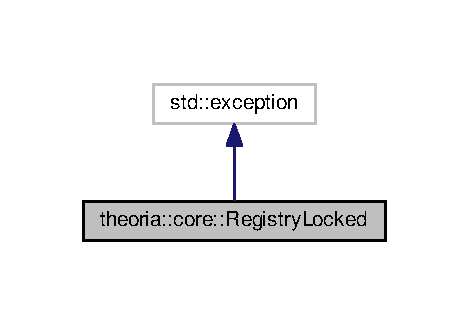
\includegraphics[width=225pt]{classtheoria_1_1core_1_1RegistryLocked__inherit__graph}
\end{center}
\end{figure}


Collaboration diagram for theoria\+:\+:core\+:\+:Registry\+Locked\+:\nopagebreak
\begin{figure}[H]
\begin{center}
\leavevmode
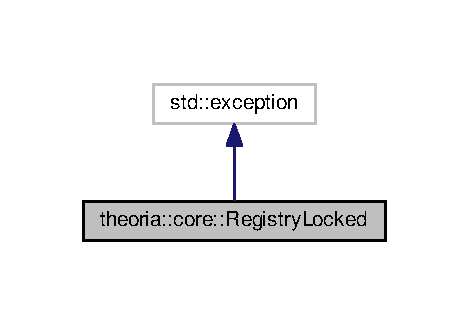
\includegraphics[width=225pt]{classtheoria_1_1core_1_1RegistryLocked__coll__graph}
\end{center}
\end{figure}


The documentation for this class was generated from the following file\+:\begin{DoxyCompactItemize}
\item 
include/theoria/core/Registry.\+h\end{DoxyCompactItemize}

\hypertarget{classtheoria_1_1core_1_1Theoria}{\section{theoria\+:\+:core\+:\+:Theoria Class Reference}
\label{classtheoria_1_1core_1_1Theoria}\index{theoria\+::core\+::\+Theoria@{theoria\+::core\+::\+Theoria}}
}
\subsection*{Public Member Functions}
\begin{DoxyCompactItemize}
\item 
\hypertarget{classtheoria_1_1core_1_1Theoria_ae8537946e39ac2ec084332edd6ef0a9a}{void {\bfseries help} ()}\label{classtheoria_1_1core_1_1Theoria_ae8537946e39ac2ec084332edd6ef0a9a}

\item 
\hypertarget{classtheoria_1_1core_1_1Theoria_a353a71a3b26b77d814c99756a749bbdf}{void {\bfseries show\+\_\+config} (bool exit)}\label{classtheoria_1_1core_1_1Theoria_a353a71a3b26b77d814c99756a749bbdf}

\item 
\hypertarget{classtheoria_1_1core_1_1Theoria_a7c08abec5d2655e8779f81622406ccb7}{void {\bfseries init} ()}\label{classtheoria_1_1core_1_1Theoria_a7c08abec5d2655e8779f81622406ccb7}

\item 
\hypertarget{classtheoria_1_1core_1_1Theoria_a2792aa50eb3ec9a2bea5288097052a3f}{void {\bfseries run} ()}\label{classtheoria_1_1core_1_1Theoria_a2792aa50eb3ec9a2bea5288097052a3f}

\end{DoxyCompactItemize}


The documentation for this class was generated from the following files\+:\begin{DoxyCompactItemize}
\item 
include/theoria/core/Theoria.\+h\item 
src/core/Theoria.\+cpp\end{DoxyCompactItemize}

\hypertarget{classtheoria_1_1config_1_1TOMLConfigBuilder}{}\section{theoria\+:\+:config\+:\+:T\+O\+M\+L\+Config\+Builder Class Reference}
\label{classtheoria_1_1config_1_1TOMLConfigBuilder}\index{theoria\+::config\+::\+T\+O\+M\+L\+Config\+Builder@{theoria\+::config\+::\+T\+O\+M\+L\+Config\+Builder}}


Inheritance diagram for theoria\+:\+:config\+:\+:T\+O\+M\+L\+Config\+Builder\+:
\nopagebreak
\begin{figure}[H]
\begin{center}
\leavevmode
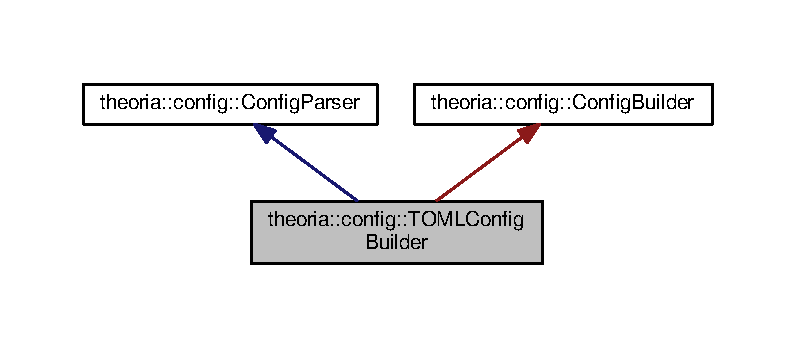
\includegraphics[width=350pt]{classtheoria_1_1config_1_1TOMLConfigBuilder__inherit__graph}
\end{center}
\end{figure}


Collaboration diagram for theoria\+:\+:config\+:\+:T\+O\+M\+L\+Config\+Builder\+:
\nopagebreak
\begin{figure}[H]
\begin{center}
\leavevmode
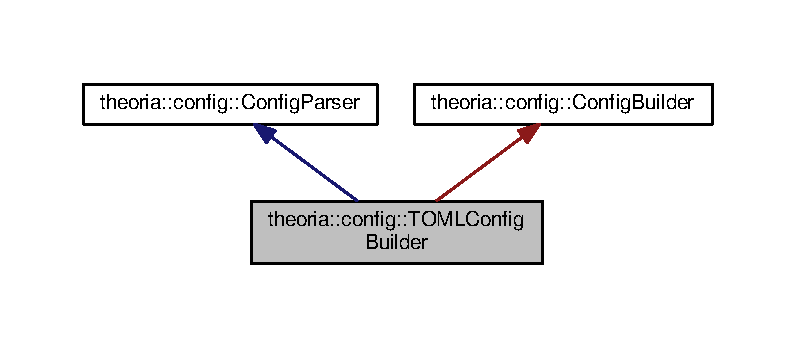
\includegraphics[width=350pt]{classtheoria_1_1config_1_1TOMLConfigBuilder__coll__graph}
\end{center}
\end{figure}
\subsection*{Public Member Functions}
\begin{DoxyCompactItemize}
\item 
std\+::unique\+\_\+ptr$<$ const \hyperlink{classtheoria_1_1config_1_1Config}{Config} $>$ \hyperlink{classtheoria_1_1config_1_1TOMLConfigBuilder_afba5445b56e12b39cf1b266627a27f58}{parse\+\_\+file} (const std\+::string \&filename) override
\item 
\mbox{\Hypertarget{classtheoria_1_1config_1_1TOMLConfigBuilder_ac5a36aebe769d67decc9946ee2a3fbc3}\label{classtheoria_1_1config_1_1TOMLConfigBuilder_ac5a36aebe769d67decc9946ee2a3fbc3}} 
std\+::unique\+\_\+ptr$<$ const \hyperlink{classtheoria_1_1config_1_1Config}{Config} $>$ {\bfseries parse} (std\+::istream \&stream) override
\end{DoxyCompactItemize}
\subsection*{Additional Inherited Members}


\subsection{Member Function Documentation}
\mbox{\Hypertarget{classtheoria_1_1config_1_1TOMLConfigBuilder_afba5445b56e12b39cf1b266627a27f58}\label{classtheoria_1_1config_1_1TOMLConfigBuilder_afba5445b56e12b39cf1b266627a27f58}} 
\index{theoria\+::config\+::\+T\+O\+M\+L\+Config\+Builder@{theoria\+::config\+::\+T\+O\+M\+L\+Config\+Builder}!parse\+\_\+file@{parse\+\_\+file}}
\index{parse\+\_\+file@{parse\+\_\+file}!theoria\+::config\+::\+T\+O\+M\+L\+Config\+Builder@{theoria\+::config\+::\+T\+O\+M\+L\+Config\+Builder}}
\subsubsection{\texorpdfstring{parse\+\_\+file()}{parse\_file()}}
{\footnotesize\ttfamily std\+::unique\+\_\+ptr$<$ const \hyperlink{classtheoria_1_1config_1_1Config}{Config} $>$ T\+O\+M\+L\+Config\+Builder\+::parse\+\_\+file (\begin{DoxyParamCaption}\item[{const std\+::string \&}]{filename }\end{DoxyParamCaption})\hspace{0.3cm}{\ttfamily [override]}, {\ttfamily [virtual]}}

Default implementation opens the file and calls parse(with the file\textquotesingle{}s std\+::ifstream)

the file to parse \begin{DoxyReturn}{Returns}
the resulting \hyperlink{classtheoria_1_1config_1_1Config}{Config} object
\end{DoxyReturn}
N\+O\+TE\+:\+: If you override parse\+\_\+file in your derived \hyperlink{classtheoria_1_1config_1_1ConfigParser}{Config\+Parser} then you can optionally implement parse or simply stub it out as Theoria will only call parse\+\_\+file directly. A stream-\/based interface is useful for writing unit tests using istringstream. 

Reimplemented from \hyperlink{classtheoria_1_1config_1_1ConfigParser_a4eca80a9831324237f2a2aa9a5018c89}{theoria\+::config\+::\+Config\+Parser}.



The documentation for this class was generated from the following files\+:\begin{DoxyCompactItemize}
\item 
include/theoria/config/T\+O\+M\+L\+Config\+Builder.\+h\item 
src/config/T\+O\+M\+L\+Config\+Builder.\+cpp\end{DoxyCompactItemize}

\hypertarget{classtheoria_1_1core_1_1TOMLConfigBuilderComp}{}\section{theoria\+:\+:core\+:\+:T\+O\+M\+L\+Config\+Builder\+Comp Class Reference}
\label{classtheoria_1_1core_1_1TOMLConfigBuilderComp}\index{theoria\+::core\+::\+T\+O\+M\+L\+Config\+Builder\+Comp@{theoria\+::core\+::\+T\+O\+M\+L\+Config\+Builder\+Comp}}


{\ttfamily \#include $<$Core\+Components.\+h$>$}



Inheritance diagram for theoria\+:\+:core\+:\+:T\+O\+M\+L\+Config\+Builder\+Comp\+:\nopagebreak
\begin{figure}[H]
\begin{center}
\leavevmode
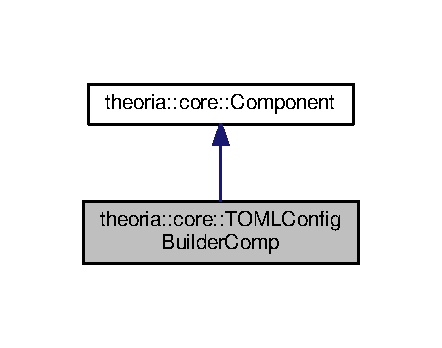
\includegraphics[width=212pt]{classtheoria_1_1core_1_1TOMLConfigBuilderComp__inherit__graph}
\end{center}
\end{figure}


Collaboration diagram for theoria\+:\+:core\+:\+:T\+O\+M\+L\+Config\+Builder\+Comp\+:\nopagebreak
\begin{figure}[H]
\begin{center}
\leavevmode
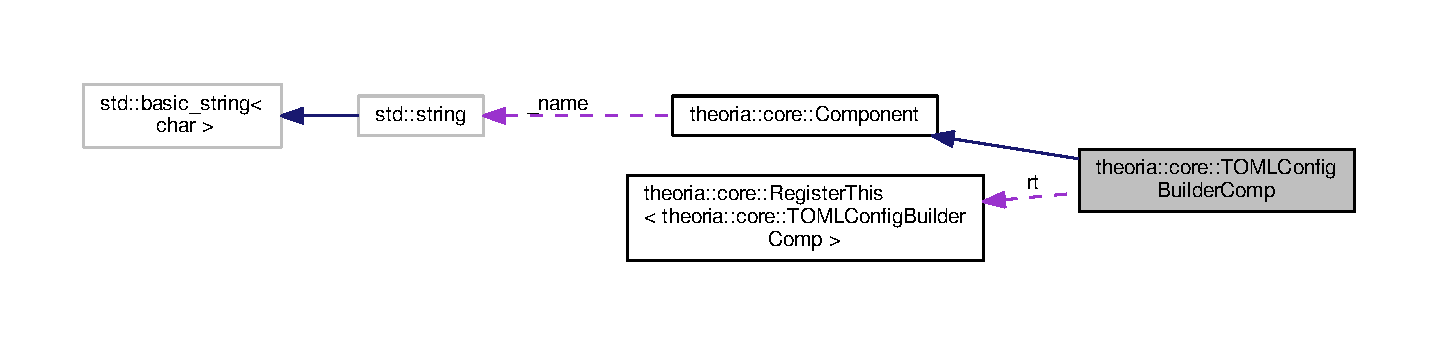
\includegraphics[width=350pt]{classtheoria_1_1core_1_1TOMLConfigBuilderComp__coll__graph}
\end{center}
\end{figure}
\subsection*{Public Member Functions}
\begin{DoxyCompactItemize}
\item 
\hyperlink{classtheoria_1_1core_1_1TOMLConfigBuilderComp_a7944116685d64329a987f6dd3f0f8f17}{T\+O\+M\+L\+Config\+Builder\+Comp} (Comp\+Id \hyperlink{classtheoria_1_1core_1_1Component_ab539df9f996efceda7743fa1b69cd25d}{id})
\item 
\hyperlink{classtheoria_1_1core_1_1Component}{Component} $\ast$ \hyperlink{classtheoria_1_1core_1_1TOMLConfigBuilderComp_a7cfce41f96c49af8e80d884f70ee66fa}{acquire} (const std\+::type\+\_\+info \&type\+Info, void $\ast$$\ast$dest) override
\end{DoxyCompactItemize}
\subsection*{Static Public Member Functions}
\begin{DoxyCompactItemize}
\item 
static \hyperlink{classtheoria_1_1core_1_1Component}{Component} $\ast$ \hyperlink{classtheoria_1_1core_1_1TOMLConfigBuilderComp_abb82664199a9549fddb64bc442a5ddfa}{factory} (Comp\+Id \hyperlink{classtheoria_1_1core_1_1Component_ab539df9f996efceda7743fa1b69cd25d}{id})
\end{DoxyCompactItemize}
\subsection*{Static Public Attributes}
\begin{DoxyCompactItemize}
\item 
static D\+L\+L\+\_\+\+P\+U\+B\+L\+IC \hyperlink{classtheoria_1_1core_1_1RegisterThis}{Register\+This}$<$ \hyperlink{classtheoria_1_1core_1_1TOMLConfigBuilderComp}{T\+O\+M\+L\+Config\+Builder\+Comp} $>$ \hyperlink{classtheoria_1_1core_1_1TOMLConfigBuilderComp_abba84fd2e773b9ab26692c9638a1dcc4}{rt}
\end{DoxyCompactItemize}
\subsection*{Additional Inherited Members}


\subsection{Detailed Description}
\hyperlink{classtheoria_1_1core_1_1Component}{Component} wrapper to T\+O\+M\+L\+Config\+Builder 

\subsection{Constructor \& Destructor Documentation}
\mbox{\Hypertarget{classtheoria_1_1core_1_1TOMLConfigBuilderComp_a7944116685d64329a987f6dd3f0f8f17}\label{classtheoria_1_1core_1_1TOMLConfigBuilderComp_a7944116685d64329a987f6dd3f0f8f17}} 
\index{theoria\+::core\+::\+T\+O\+M\+L\+Config\+Builder\+Comp@{theoria\+::core\+::\+T\+O\+M\+L\+Config\+Builder\+Comp}!T\+O\+M\+L\+Config\+Builder\+Comp@{T\+O\+M\+L\+Config\+Builder\+Comp}}
\index{T\+O\+M\+L\+Config\+Builder\+Comp@{T\+O\+M\+L\+Config\+Builder\+Comp}!theoria\+::core\+::\+T\+O\+M\+L\+Config\+Builder\+Comp@{theoria\+::core\+::\+T\+O\+M\+L\+Config\+Builder\+Comp}}
\subsubsection{\texorpdfstring{T\+O\+M\+L\+Config\+Builder\+Comp()}{TOMLConfigBuilderComp()}}
{\footnotesize\ttfamily theoria\+::core\+::\+T\+O\+M\+L\+Config\+Builder\+Comp\+::\+T\+O\+M\+L\+Config\+Builder\+Comp (\begin{DoxyParamCaption}\item[{Comp\+Id}]{id }\end{DoxyParamCaption})\hspace{0.3cm}{\ttfamily [inline]}}

\hyperlink{classtheoria_1_1core_1_1Component}{Component} constructor 

\subsection{Member Function Documentation}
\mbox{\Hypertarget{classtheoria_1_1core_1_1TOMLConfigBuilderComp_a7cfce41f96c49af8e80d884f70ee66fa}\label{classtheoria_1_1core_1_1TOMLConfigBuilderComp_a7cfce41f96c49af8e80d884f70ee66fa}} 
\index{theoria\+::core\+::\+T\+O\+M\+L\+Config\+Builder\+Comp@{theoria\+::core\+::\+T\+O\+M\+L\+Config\+Builder\+Comp}!acquire@{acquire}}
\index{acquire@{acquire}!theoria\+::core\+::\+T\+O\+M\+L\+Config\+Builder\+Comp@{theoria\+::core\+::\+T\+O\+M\+L\+Config\+Builder\+Comp}}
\subsubsection{\texorpdfstring{acquire()}{acquire()}}
{\footnotesize\ttfamily \hyperlink{classtheoria_1_1core_1_1Component}{Component} $\ast$ T\+O\+M\+L\+Config\+Builder\+Comp\+::acquire (\begin{DoxyParamCaption}\item[{const std\+::type\+\_\+info \&}]{type\+Info,  }\item[{void $\ast$$\ast$}]{dest }\end{DoxyParamCaption})\hspace{0.3cm}{\ttfamily [override]}, {\ttfamily [virtual]}}

Used to acquire underlying resolver 

Reimplemented from \hyperlink{classtheoria_1_1core_1_1Component_a18744abc83e088af3c3d42e0a22c35e3}{theoria\+::core\+::\+Component}.

\mbox{\Hypertarget{classtheoria_1_1core_1_1TOMLConfigBuilderComp_abb82664199a9549fddb64bc442a5ddfa}\label{classtheoria_1_1core_1_1TOMLConfigBuilderComp_abb82664199a9549fddb64bc442a5ddfa}} 
\index{theoria\+::core\+::\+T\+O\+M\+L\+Config\+Builder\+Comp@{theoria\+::core\+::\+T\+O\+M\+L\+Config\+Builder\+Comp}!factory@{factory}}
\index{factory@{factory}!theoria\+::core\+::\+T\+O\+M\+L\+Config\+Builder\+Comp@{theoria\+::core\+::\+T\+O\+M\+L\+Config\+Builder\+Comp}}
\subsubsection{\texorpdfstring{factory()}{factory()}}
{\footnotesize\ttfamily \hyperlink{classtheoria_1_1core_1_1Component}{Component} $\ast$ T\+O\+M\+L\+Config\+Builder\+Comp\+::factory (\begin{DoxyParamCaption}\item[{Comp\+Id}]{id }\end{DoxyParamCaption})\hspace{0.3cm}{\ttfamily [static]}}

Factory for this component 

\subsection{Member Data Documentation}
\mbox{\Hypertarget{classtheoria_1_1core_1_1TOMLConfigBuilderComp_abba84fd2e773b9ab26692c9638a1dcc4}\label{classtheoria_1_1core_1_1TOMLConfigBuilderComp_abba84fd2e773b9ab26692c9638a1dcc4}} 
\index{theoria\+::core\+::\+T\+O\+M\+L\+Config\+Builder\+Comp@{theoria\+::core\+::\+T\+O\+M\+L\+Config\+Builder\+Comp}!rt@{rt}}
\index{rt@{rt}!theoria\+::core\+::\+T\+O\+M\+L\+Config\+Builder\+Comp@{theoria\+::core\+::\+T\+O\+M\+L\+Config\+Builder\+Comp}}
\subsubsection{\texorpdfstring{rt}{rt}}
{\footnotesize\ttfamily \hyperlink{classtheoria_1_1core_1_1RegisterThis}{Register\+This}$<$ \hyperlink{classtheoria_1_1core_1_1TOMLConfigBuilderComp}{T\+O\+M\+L\+Config\+Builder\+Comp} $>$ T\+O\+M\+L\+Config\+Builder\+Comp\+::rt\hspace{0.3cm}{\ttfamily [static]}}

Register factory 

The documentation for this class was generated from the following files\+:\begin{DoxyCompactItemize}
\item 
include/theoria/core/Core\+Components.\+h\item 
src/core/Core\+Components.\+cpp\end{DoxyCompactItemize}

\hypertarget{classtheoria_1_1config_1_1TOMLResolver}{\section{theoria\+:\+:config\+:\+:T\+O\+M\+L\+Resolver Class Reference}
\label{classtheoria_1_1config_1_1TOMLResolver}\index{theoria\+::config\+::\+T\+O\+M\+L\+Resolver@{theoria\+::config\+::\+T\+O\+M\+L\+Resolver}}
}


Inheritance diagram for theoria\+:\+:config\+:\+:T\+O\+M\+L\+Resolver\+:
\nopagebreak
\begin{figure}[H]
\begin{center}
\leavevmode
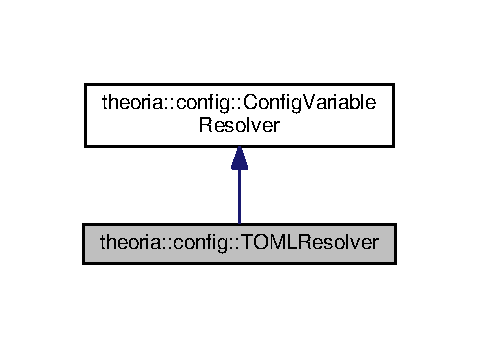
\includegraphics[width=230pt]{classtheoria_1_1config_1_1TOMLResolver__inherit__graph}
\end{center}
\end{figure}


Collaboration diagram for theoria\+:\+:config\+:\+:T\+O\+M\+L\+Resolver\+:
\nopagebreak
\begin{figure}[H]
\begin{center}
\leavevmode
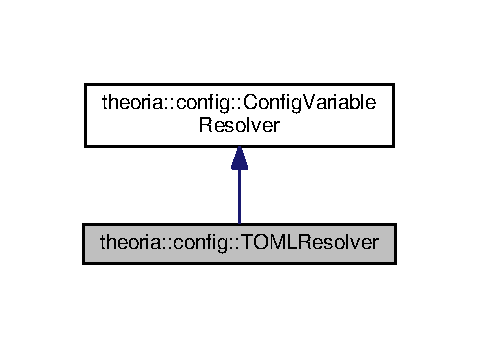
\includegraphics[width=230pt]{classtheoria_1_1config_1_1TOMLResolver__coll__graph}
\end{center}
\end{figure}
\subsection*{Classes}
\begin{DoxyCompactItemize}
\item 
class \hyperlink{classTOMLResolver_1_1TOMLResolverImpl}{T\+O\+M\+L\+Resolver\+Impl}
\end{DoxyCompactItemize}
\subsection*{Public Member Functions}
\begin{DoxyCompactItemize}
\item 
\hypertarget{classtheoria_1_1config_1_1TOMLResolver_a94a2659c23a5c85d05fb62e67c8c7810}{{\bfseries T\+O\+M\+L\+Resolver} (const std\+::string \&toml\+File\+Path)}\label{classtheoria_1_1config_1_1TOMLResolver_a94a2659c23a5c85d05fb62e67c8c7810}

\item 
\hypertarget{classtheoria_1_1config_1_1TOMLResolver_a2772b7d149cabddd2b622b786720420f}{{\bfseries T\+O\+M\+L\+Resolver} (std\+::istream \&is)}\label{classtheoria_1_1config_1_1TOMLResolver_a2772b7d149cabddd2b622b786720420f}

\item 
\hypertarget{classtheoria_1_1config_1_1TOMLResolver_a42daff166eca2c9c9dd77868faf0122d}{Result {\bfseries lookup} (const std\+::string \&name) const override}\label{classtheoria_1_1config_1_1TOMLResolver_a42daff166eca2c9c9dd77868faf0122d}

\item 
\hypertarget{classtheoria_1_1config_1_1TOMLResolver_a6b50ff1e396f74183318915e602837fc}{virtual std\+::string {\bfseries name} () const override}\label{classtheoria_1_1config_1_1TOMLResolver_a6b50ff1e396f74183318915e602837fc}

\end{DoxyCompactItemize}
\subsection*{Additional Inherited Members}


The documentation for this class was generated from the following files\+:\begin{DoxyCompactItemize}
\item 
include/theoria/config/Resolve.\+h\item 
src/config/Resolve.\+cpp\end{DoxyCompactItemize}

\hypertarget{classTOMLResolver_1_1TOMLResolverImpl}{\section{theoria\+:\+:config\+:\+:T\+O\+M\+L\+Resolver\+:\+:T\+O\+M\+L\+Resolver\+Impl Class Reference}
\label{classTOMLResolver_1_1TOMLResolverImpl}\index{theoria\+::config\+::\+T\+O\+M\+L\+Resolver\+::\+T\+O\+M\+L\+Resolver\+Impl@{theoria\+::config\+::\+T\+O\+M\+L\+Resolver\+::\+T\+O\+M\+L\+Resolver\+Impl}}
}


Inheritance diagram for theoria\+:\+:config\+:\+:T\+O\+M\+L\+Resolver\+:\+:T\+O\+M\+L\+Resolver\+Impl\+:
\nopagebreak
\begin{figure}[H]
\begin{center}
\leavevmode
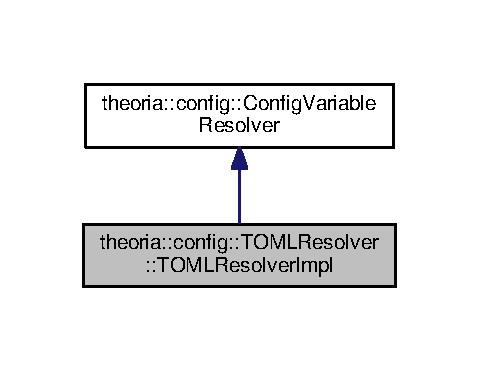
\includegraphics[width=230pt]{classTOMLResolver_1_1TOMLResolverImpl__inherit__graph}
\end{center}
\end{figure}


Collaboration diagram for theoria\+:\+:config\+:\+:T\+O\+M\+L\+Resolver\+:\+:T\+O\+M\+L\+Resolver\+Impl\+:
\nopagebreak
\begin{figure}[H]
\begin{center}
\leavevmode
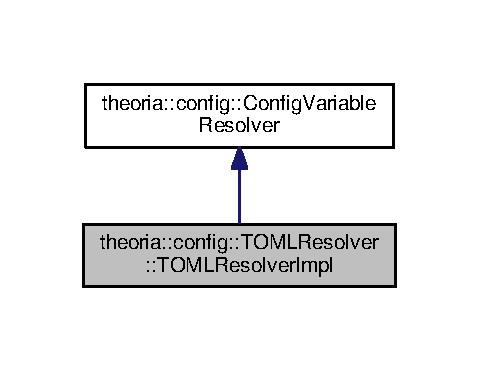
\includegraphics[width=230pt]{classTOMLResolver_1_1TOMLResolverImpl__coll__graph}
\end{center}
\end{figure}
\subsection*{Public Member Functions}
\begin{DoxyCompactItemize}
\item 
\hypertarget{classTOMLResolver_1_1TOMLResolverImpl_a297c93ec008519e79192844d483273ac}{{\bfseries T\+O\+M\+L\+Resolver\+Impl} (const std\+::string \&toml\+File\+Path)}\label{classTOMLResolver_1_1TOMLResolverImpl_a297c93ec008519e79192844d483273ac}

\item 
\hypertarget{classTOMLResolver_1_1TOMLResolverImpl_acee3fe2b048200875c6ee00aacad76ac}{{\bfseries T\+O\+M\+L\+Resolver\+Impl} (std\+::istream \&is)}\label{classTOMLResolver_1_1TOMLResolverImpl_acee3fe2b048200875c6ee00aacad76ac}

\item 
\hypertarget{classTOMLResolver_1_1TOMLResolverImpl_aebc6940c543f3b12484aa2735a6fcf1b}{Result {\bfseries lookup} (const std\+::string \&name) const override}\label{classTOMLResolver_1_1TOMLResolverImpl_aebc6940c543f3b12484aa2735a6fcf1b}

\item 
\hypertarget{classTOMLResolver_1_1TOMLResolverImpl_a5b9f36aca6c20a81b18b078fa74c3c14}{std\+::string {\bfseries name} () const override}\label{classTOMLResolver_1_1TOMLResolverImpl_a5b9f36aca6c20a81b18b078fa74c3c14}

\end{DoxyCompactItemize}
\subsection*{Additional Inherited Members}


The documentation for this class was generated from the following file\+:\begin{DoxyCompactItemize}
\item 
src/config/Resolve.\+cpp\end{DoxyCompactItemize}

\hypertarget{structtoTomlName}{}\section{to\+Toml\+Name Struct Reference}
\label{structtoTomlName}\index{to\+Toml\+Name@{to\+Toml\+Name}}


Collaboration diagram for to\+Toml\+Name\+:\nopagebreak
\begin{figure}[H]
\begin{center}
\leavevmode
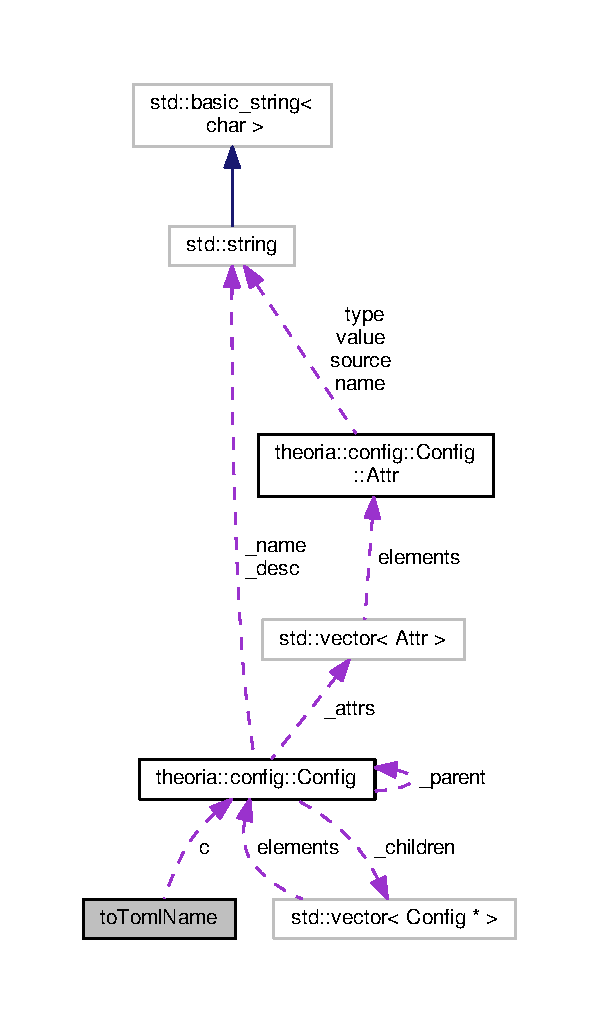
\includegraphics[width=288pt]{structtoTomlName__coll__graph}
\end{center}
\end{figure}
\subsection*{Public Member Functions}
\begin{DoxyCompactItemize}
\item 
\mbox{\Hypertarget{structtoTomlName_af8c07f9b89f61b4c54e942c0bfe3e544}\label{structtoTomlName_af8c07f9b89f61b4c54e942c0bfe3e544}} 
{\bfseries to\+Toml\+Name} (const \hyperlink{classtheoria_1_1config_1_1Config}{Config} \&c\+\_\+)
\end{DoxyCompactItemize}
\subsection*{Public Attributes}
\begin{DoxyCompactItemize}
\item 
\mbox{\Hypertarget{structtoTomlName_ac218bcee1d45d3e7a13da755b42bf19a}\label{structtoTomlName_ac218bcee1d45d3e7a13da755b42bf19a}} 
const \hyperlink{classtheoria_1_1config_1_1Config}{Config} \& {\bfseries c}
\end{DoxyCompactItemize}


\subsection{Detailed Description}
Wrapper to assist streaming a toml name 

The documentation for this struct was generated from the following file\+:\begin{DoxyCompactItemize}
\item 
src/config/Config.\+cpp\end{DoxyCompactItemize}

%--- End generated contents ---

% Index
\backmatter
\newpage
\phantomsection
\clearemptydoublepage
\addcontentsline{toc}{chapter}{Index}
\printindex

\end{document}
